\documentclass[11pt]{memoireuqam}

%%%%%%%%%%%%%%%%%%%%%%%%%%%%%%%%%%%
% OVERLEAF: Utiliser TexLive 2021 %
%%%%%%%%%%%%%%%%%%%%%%%%%%%%%%%%%%%

\usepackage[round,authoryear]{natbib}  % citations APA (Auteur, Année) -- style UQAM

\usepackage[french]{babel}
% Forcer "Tableau" partout (babel français utilise "Table" par défaut)
\addto\captionsfrench{%
  \renewcommand{\tablename}{Tableau}%
  \renewcommand{\figurename}{Figure}%
}
% LuaLaTeX gère UTF-8 nativement; inputenc serait redondant et ignoré.
\usepackage[T1]{fontenc}
\usepackage{silence}
% Avertissements bénins de la finalisation PDF/A : pdfx force le modèle couleur
% RGB (exigence PDF/A) et recharge xcolor avec une option obsolète sans effet.
% Filtres déclarés AVANT pdfx pour qu'ils soient actifs au chargement.
\WarningFilter{xcolor}{Package option `hyperref' is obsolete}
\WarningFilter{pdfx}{Setting all color commands to rgb}
\usepackage{url}
% --- Finalisation PDF/A-1b (dépôt UQAM / Archipel) ---
% pdfx charge lui-même hyperref ; on lui transmet les options AVANT son chargement
% pour éviter un « option clash » (ne pas charger hyperref séparément ensuite).
\PassOptionsToPackage{hypertexnames=false}{hyperref}
\usepackage[a-1b]{pdfx}

\usepackage{graphicx}
\usepackage{pdflscape}      % pages paysage lisibles à l'écran et à l'impression
\usepackage{eso-pic}        % folio repositionné sur la page paysage (voir chapitre 6)
\usepackage{amsfonts}
\usepackage{amsmath}         % \text{} dans les équations
\usepackage{enumitem}        % options [leftmargin=...] dans enumerate
\usepackage{booktabs}       % tableaux professionnels
\usepackage{multirow}       % cellules fusionnées
\usepackage{longtable}      % tableaux qui se brisent sur plusieurs pages
\usepackage{array}          % colonnes personnalisées
% Interligne des tableaux, valeur unique pour tout le mémoire. Sans elle, les
% lignes se touchaient presque : les tableaux longs paraissaient plus denses que
% les courts, alors que leur espacement etait identique. Aucun tableau ne doit
% redéfinir localement \arraystretch, sous peine de rompre cette uniformité.
\renewcommand{\arraystretch}{1.15}
\usepackage{float}          % option [H] pour certains flottants
% Pseudocodes en algorithme numerote (gabarit du codirecteur). Les mots-cles sont
% francises car algorithm2e affiche Input/Output par defaut, et le compteur suit le
% chapitre comme le reste du memoire.
\usepackage[ruled,vlined,linesnumbered]{algorithm2e}
\SetAlgorithmName{Algorithme}{algorithme}{Liste des algorithmes}
\SetKwInput{KwIn}{Entrée}
\SetKwInput{KwOut}{Sortie}
\SetKw{KwEt}{et}
\SetKwFor{PourChaque}{pour chaque}{faire}{fin}
\SetKwIF{Si}{SinonSi}{Sinon}{si}{alors}{sinon si}{sinon}{fin}
\SetAlgoCaptionSeparator{.}
\renewcommand{\thealgocf}{\thechapter.\arabic{algocf}}
\counterwithin*{algocf}{chapter}
\usepackage{tikz}           % diagrammes
\usetikzlibrary{arrows.meta, positioning, shapes.geometric, fit, calc, decorations.pathreplacing, backgrounds}
\usepackage{pgfplots}       % graphiques de données
\pgfplotsset{compat=1.18}
\usepgfplotslibrary{fillbetween}
\usetikzlibrary{patterns}    % hachures dans les bar charts

\usepackage{placeins}       % \FloatBarrier pour éviter les chevauchements
\usepackage{xcolor}         % couleurs personnalisées
% --- Palette professionnelle (inspirée Tableau / Nature) ---
\definecolor{ifblue}{RGB}{55,90,127}       % bleu marine sobre
\definecolor{loforange}{RGB}{190,120,50}   % terre cuite douce
\definecolor{rulegreen}{RGB}{75,135,100}   % vert sauge
\definecolor{rawred}{RGB}{175,70,70}       % rouge brique atténué
\definecolor{profgray}{RGB}{130,130,130}   % gris neutre

% Police similaire à Calibri
\usepackage[sfdefault,lf]{carlito}
% \usepackage{times}
\emergencystretch=2em
\hfuzz=10pt
\hbadness=10000
\vbadness=10000
% \citep et \citet sont définis nativement par natbib

% Nettoie les avertissements purement typographiques de Carlito.
\WarningFilter{latexfont}{Font shape `T1/Crlt-LF/m/sc' undefined}
\WarningFilter{latexfont}{Font shape `TU/Carlito(0)/m/sc' undefined}
\WarningFilter{latexfont}{Some font shapes were not available, defaults substituted}
% Avertissement bénin de babel-french sur les légendes, sans impact sur le PDF courant.
\WarningFilter{french3.ldf}{Figures' and tables' captions might look like}

% Espacement des figures rendu rigide. La classe fixe deja parskip a
% 18bp plus 2bp minus 2bp : c'est l'espace entre paragraphes qui sert de
% ressort de remplissage de page. L'elasticite de intextsep (12pt plus 2pt
% minus 2pt) vient de la classe book et faisait varier de 2,8bp le blanc
% autour des figures d'une page a l'autre. On la supprime et on exprime la
% valeur en bp, l'unite retenue par la classe.
\setlength{\intextsep}{12bp}
\setlength{\textfloatsep}{12bp}
\setlength{\floatsep}{12bp}
% parskip est declare 18bp plus 2bp minus 2bp par la classe, et redeclare a
% chaque tete de chapitre. On conserve la valeur choisie par la classe et on
% retire seulement l'elasticite, de sorte que chaque paragraphe recoive
% exactement les 18bp prevus au lieu de 16 a 20bp selon le remplissage.
\usepackage{etoolbox}
\makeatletter
\apptocmd{\@makechapterhead}{\parskip=18bp\relax}{}{}
\apptocmd{\@makeschapterhead}{\parskip=18bp\relax}{}{}
\makeatother
\setlength{\parskip}{18bp}

% Le format des citations et des labels est géré par natbib + apalike-uqam


\begin{document}

%%%%%%%%%%%%%%%%%%%%
% Pour la page titre
%%%%%%%%%%%%%%%%%%%%
\title{Détection temporelle de dégradations comportementales associées au risque de boiterie chez les vaches laitières}
% Votre nom complet tel qu'il apparaît à votre dossier du registrariat de l'UQAM
\author{Aliou Barry}
% Année et mois courant sauf si spécifié autrement pas \degreemonth et \degreeyear
%\degreemonth{mois du dépôt}
%\degreeyear{année du dépôt}
\uqammemoire %% ou \uqamthese ou \uqamrapport ou \uqamprop 
\matiere{informatique}
\concentration{Concentration : systèmes électroniques}


\pagenumbering{roman} % numérotation des pages en chiffres romains
\thispagestyle{empty}        % La page titre n'est pas numérotée
\maketitle
\stepcounter{page}

%%%%%%%%%%%%%%%%%%%%
% Page préliminaires
%%%%%%%%%%%%%%%%%%%%

\chapter*{}
\thispagestyle{empty}

\vspace*{\fill}

\begin{flushright}
\textit{À la mémoire de mon père,\\
dont l'exemple, les valeurs et la confiance\\
guident encore chacun de mes pas.}

\vspace{1.5em}

\textit{À ma mère,\\
qui veille sur nous,\\
et qui fait, sans jamais le dire,\\
bien plus que ce que l'on peut demander.}

\vspace{1.5em}

\textit{À mes petits frères et sœurs,\\
Aissatou, Ibrahima et Hassatou.\\
Vous avez traversé la même épreuve\\
sans cesser d'avancer.\\
Ce chemin est aussi le vôtre,\\
et j'espère seulement\\
vous en avoir ouvert un bout.}
\end{flushright}

\vspace*{\fill}

\chapter*{Remerciements}

Je tiens à exprimer ma profonde gratitude envers mon directeur de recherche, le professeur
Abdoulaye Baniré Diallo, pour son encadrement scientifique rigoureux, sa confiance et sa
disponibilité tout au long de ce projet~; ses conseils méthodologiques et sa vision ont été
déterminants dans l'aboutissement de ce mémoire. Je remercie également mon codirecteur,
Zakaria El Alaoui Ismaili, pour son accompagnement, ses retours constructifs et son
expertise, qui ont enrichi ce travail à chaque étape.

Ce mémoire a été réalisé au sein du Laboratoire de bio-informatique de l'UQAM, un
environnement de recherche stimulant et collaboratif, dans le cadre du projet Well-E
regroupant des chercheurs de l'UQAM et de McGill, dont le cadre applicatif et les données ont
rendu ce travail possible. Je remercie l'ensemble des membres du laboratoire pour les
échanges scientifiques et le soutien quotidien, et plus particulièrement mes collègues
Francois, Armand, Issa, Khaly, Nicolas, Amanda et Awa, dont la camaraderie et l'entraide ont
ponctué ces années de maîtrise.

Je remercie les membres du jury pour le temps consacré à l'évaluation de ce mémoire et pour
leurs commentaires constructifs.

Enfin, je remercie ma famille et mes proches pour leur soutien indéfectible et leurs
encouragements constants.

\tableofcontents % Pour générer la table des matières
\listoffigures
\listoftables
\chapter*{Liste des acronymes et abréviations}
\addcontentsline{toc}{chapter}{Liste des acronymes et abréviations}

\begin{longtable}{@{}lp{11cm}@{}}
\textbf{AUC} & \textit{Area Under the Curve}: aire sous la courbe ROC utilisée ici comme mesure descriptive exploratoire \\[3pt]
\textbf{CSV} & \textit{Comma-Separated Values}: format de fichier tabulaire \\[3pt]
\textbf{CUSUM} & \textit{Cumulative Sum}: somme cumulative pour la détection de changements persistants \\[3pt]
\textbf{FAIR} & \textit{Findable, Accessible, Interoperable, Reusable}: principes de gestion des données scientifiques \\[3pt]
\textbf{IF} & \textit{Isolation Forest}: algorithme de détection d'anomalies par isolation \\[3pt]
\textbf{HYPO} & Branche temporelle recherchant une baisse persistante et multivariée de l'activité \\[3pt]
\textbf{INSTABILITÉ} & Branche temporelle recherchant un mouvement disproportionné, des transitions denses et une posture fragmentée \\[3pt]
\textbf{IoU} & \textit{Intersection over Union}: mesure de recouvrement temporel \\[3pt]
\textbf{JSON} & \textit{JavaScript Object Notation}: format d'échange de données \\[3pt]
\textbf{LOF} & \textit{Local Outlier Factor}: détecteur d'anomalies fondé sur la densité locale \\[3pt]
\textbf{MAD} & \textit{Median Absolute Deviation}: écart absolu médian \\[3pt]
\textbf{MI} & \textit{Motion Index}: indice de mouvement fourni par le capteur \\[3pt]
\textbf{PLF} & \textit{Precision Livestock Farming}: élevage de précision \\[3pt]
\textbf{SHA-256} & Fonction de hachage cryptographique utilisée pour vérifier l'intégrité des artefacts \\[3pt]
\textbf{SLS} & Score observationnel de la cohorte IceTag--SLS, somme de quatre composantes binaires dans les fichiers étudiés \\[3pt]
\end{longtable}

\newpage

\noindent\textbf{Termes techniques}

\vspace{0.5em}

\begin{tabular}{@{}lp{10cm}@{}}
\textbf{Alerte comportementale} & Signal indiquant une dégradation persistante de plusieurs familles de mesures; elle doit être vérifiée et n'est pas un diagnostic \\[3pt]
\textbf{Période de référence} & Partie initiale de la série d'une vache utilisée pour estimer son comportement attendu \\[3pt]
\textbf{Boiterie} & Altération de la locomotion dont l'évaluation clinique repose sur la démarche, la posture, l'appui et, au besoin, l'examen du pied \\[3pt]
\textbf{Couverture} & Proportion des mesures attendues effectivement observées dans un intervalle \\[3pt]
\textbf{Créneau horaire} & Position dans le cycle journalier utilisée pour comparer un signal à des périodes homologues de la période de référence \\[3pt]
\textbf{Événement en période future} & Perturbation injectée uniquement après la partie utilisée pour construire la référence \\[3pt]
\textbf{Inspection visuelle} & Contrôle humain de la cohérence technique des événements et des sorties, sans adjudication clinique \\[3pt]
\textbf{Notification de fond} & Notification observée hors fenêtre injectée sur des données non étiquetées; elle ne peut être qualifiée de vraie ou fausse alerte clinique \\[3pt]
\textbf{Notification de vérification} & Sortie de priorité 2 ou 3 demandant une observation ciblée de l'animal, sans conclure à une boiterie \\[3pt]
\textbf{Période réfractaire} & Durée minimale entre deux notifications; elle dépend de la branche et vaut 12 heures pour la fusion principale \\[3pt]
\textbf{Chaîne de traitement (pipeline)} & Suite des opérations allant de l'ingestion des données aux épisodes et aux notifications \\[3pt]
\end{tabular}

\chapter*{Liste des symboles}
\addcontentsline{toc}{chapter}{Liste des symboles}

\begin{tabular}{@{}lp{13.5cm}@{}}
$r_{j,t}$ & Ratio entre le signal agrégé observé et sa référence attendue pour la famille $j$ au temps $t$ \\[3pt]
$d_{j,t}$ & Déficit unilatéral d'une famille d'activité: $\max(0,1-r_{j,t})$ \\[3pt]
$p_t$ & Composante posturale combinant excès de temps couché et diminution du temps debout \\[3pt]
$s_t$ & Score instantané de dégradation comportementale, borné entre 0 et 1 et non interprétable comme une probabilité clinique \\[3pt]
$e_t$ & Évidence temporelle issue du score et de la baisse progressive \\[3pt]
$C_t$ & Somme cumulative unilatérale (CUSUM) au temps $t$ \\[3pt]
$k$ & Dérive soustraite à chaque mise à jour du CUSUM \\[3pt]
$E$ & Fenêtre temporelle d'un événement injecté \\[3pt]
$A$ & Épisode d'alerte produit par le détecteur \\[3pt]
$\mathrm{IoU}$ & \textit{Intersection over Union}: $\frac{|E\cap A|}{|E\cup A|}$, mesure du recouvrement temporel \\[3pt]
$n$ & Nombre d'unités statistiques ou d'événements, selon le tableau \\[3pt]
$\rho$ & Coefficient de corrélation de rang de Spearman \\[3pt]
\end{tabular}


\begin{abstract}
\noindent
La boiterie demeure un problème majeur de bien-être et de performance en élevage laitier. Son
repérage repose sur l'observation humaine et le score locomoteur, indispensables, mais difficiles
à maintenir en continu sur un troupeau. Les capteurs d'activité complètent cette surveillance en
signalant des changements comportementaux persistants qui justifient une vérification sur le terrain.
Ce mémoire conçoit et évalue un système reproductible d'\textbf{alerte comportementale précoce}
à partir de capteurs IceQube fixés à la patte.

La contribution principale repose sur la branche temporelle HYPO. Elle compare le comportement
actuel de chaque vache à celui observé pendant sa propre période de référence et recherche une
baisse graduelle, persistante et concordante de
plusieurs familles de signaux: pas, indice de mouvement (\textit{Motion Index}), transitions
posturales, temps couché et temps debout. Cette logique individualisée transforme des séries de données indirectes en priorités de
vérification traçables. L'évaluation repose sur des événements injectés uniquement après la
période de référence, puis comparés à une exécution propre de la même vache afin de ne créditer
que les alertes attribuables. Sur les dégradations graduelles, HYPO recouvre la plupart
des événements et localise mieux les épisodes qu'Isolation Forest et Local Outlier Factor; le
contrôle bref isolé est rejeté. Un test de stress sans nouveau réglage étend l'évaluation à des
départs abrupts, des familles désynchronisées, une récupération asymétrique, du bruit et un
bloc de données manquantes, à aire numérique d'enveloppe appariée. HYPO y garde son avantage sur
IF et LOF et produit moins de fond que le comparateur
pédométrique, restreint au seul canal des pas, sans le dépasser pour la
localisation des formes attendues. Sa cohérence multifamille se manifeste ailleurs: elle
l'empêche de localiser une perturbation limitée aux pas, que le comparateur pédométrique situe
correctement.

Le mémoire explore aussi une extension bidirectionnelle fondée sur une branche nommée INSTABILITÉ,
qui représente des situations où un inconfort locomoteur pourrait s'accompagner d'agitation, de
transitions plus fréquentes ou de fragmentation posturale. Elle reste séparée de HYPO.
L'instabilité isolée produit une sortie de surveillance, tandis que la notification de
vérification demeure réservée aux baisses persistantes ou aux séquences
instabilité-hypoactivité. Son évaluation quantifie le gain de couverture, la charge de
vérification et la sensibilité aux causes non locomotrices.

Une analyse IceTag-SLS synchronisée confronte enfin les sorties aux scores locomoteurs à partir
de données des capteurs strictement antérieures à l'évaluation. Les vaches aux scores les plus
élevés reçoivent davantage de notifications et l'AUC descriptive globale est élevée, mais
l'analyse exacte restreinte au groupe expérimental \textit{Exercise} demeure non concluante:
l'association reste exploratoire, faute d'un effectif suffisant de vaches à score élevé hors de
ce groupe. Le mémoire livre un détecteur temporel interprétable, une interface de priorisation
et un protocole reproductible articulant performance logicielle, hypothèse comportementale et
vérification clinique.

\vspace{1em}
\textbf{Mots-clés:} boiterie bovine, alerte comportementale, capteur IceQube, détection de
changement, élevage de précision.
\end{abstract}

\begin{otherlanguage}{english}
\renewcommand{\abstractname}{Abstract}
\begin{abstract}
\noindent
Lameness remains a major welfare and performance issue in dairy farming. Its detection relies on
human observation and locomotion scoring, essential but difficult to maintain continuously at
herd scale. Activity sensors complement this monitoring by flagging persistent behavioral
changes that justify on-farm verification. This thesis designs and evaluates a reproducible
\textbf{early behavioral-alert} system based on leg-mounted IceQube sensors.

The main contribution is the temporal HYPO branch. It compares each cow with her own baseline
period and searches for a gradual, persistent and concordant decline across several signal
families: steps, motion index, postural transitions, lying time and standing time. This
individualized logic converts indirect behavioral measurements into traceable verification priorities.
Evaluation uses events injected strictly after the baseline period and compares each injected
run with a clean run of the same cow, so that only attributable alerts are credited. On gradual
degradations, HYPO recovers most events and localizes episodes better than Isolation Forest and
Local Outlier Factor; the isolated brief variation, a single short departure from normal behavior, is rejected. A no-retuning stress test
extends the evaluation to abrupt onset, desynchronized families, asymmetric recovery, noise and
a missing-data block with matched numerical perturbation-envelope area. HYPO keeps its advantage
over IF and LOF and yields less background load than the pedometric comparator, without
surpassing it in localizing the expected shapes. Its multi-family coherence shows elsewhere: it
prevents HYPO from localizing a perturbation confined to steps, which the pedometric comparator
locates correctly. Requiring joint evidence across families is what separates this approach from
characterizing perturbations through step counts alone.

The thesis explores a bidirectional extension based on an INSTABILITY branch, which
represents situations in which locomotor discomfort could involve agitation, more frequent
transitions or fragmented posture. It remains separated from HYPO: isolated instability
produces a surveillance output, whereas verification notifications are reserved for persistent
decreases or instability-to-hypoactivity sequences. Its evaluation quantifies the gain in
coverage, the verification load and the sensitivity to non-locomotor causes.

A synchronized IceTag-SLS analysis finally compares the outputs with locomotion scores using
only sensor data collected before the evaluation. Cows with the highest scores receive more
notifications and the overall descriptive AUC is high, but the exact analysis restricted to the
\textit{Exercise} group remains inconclusive: the association stays exploratory, for want of
enough high-scoring cows outside that group. The thesis delivers an interpretable temporal
detector, a prioritization interface and a reproducible protocol connecting software performance,
behavioral hypotheses and clinical verification.

\vspace{1em}
\textbf{Keywords:} bovine lameness, behavioral alert, IceQube sensor, change detection,
precision livestock farming.
\end{abstract}
\end{otherlanguage}

% Utilisez l'environnement  abstract pour rédiger votre résumé

%%%%%%%%%%%%%%%%%%%%
% Document principal
%%%%%%%%%%%%%%%%%%%%
\pagenumbering{arabic}

% Utilisez l'environnement  introduction pour rédiger votre introduction
\begin{introduction}

La boiterie désigne une altération de la locomotion, le plus souvent causée par la douleur
d'une lésion du pied ou du membre. Elle se reconnaît cliniquement à une démarche irrégulière,
un dos voûté, une répartition inégale du poids entre les membres et une réticence à se
déplacer~; son évaluation de référence repose sur une notation locomotrice standardisée
\citep{sprecher1997lameness,chapinal2010measurement}. La boiterie est un phénomène clinique.
Les changements comportementaux mesurés par les capteurs n'en constituent qu'un reflet
indirect. Cette distinction guide l'ensemble du mémoire.

La boiterie constitue un problème majeur de bien-être animal et de performance en élevage
laitier.
Les études épidémiologiques rapportent fréquemment des prévalences de l'ordre de 20\,\% ou
davantage, avec des variations selon la population, la saison et la définition clinique
retenue \citep{whay2003assessment,cook2003prevalence}. Ses
conséquences comprennent la douleur, la baisse de production, une fertilité dégradée, des
soins supplémentaires et des réformes anticipées
\citep{green2002financial,bruijnis2010assessing}. Les estimations publiées chiffrent la
perte de production laitière à environ 360~kg par lactation chez les vaches cliniquement
boiteuses et le coût moyen d'un trouble du pied à 95~dollars américains par cas (18~\$~US
s'il est subclinique), soit de l'ordre de 75~\$~US par vache et par an à l'échelle
du troupeau. Au-delà du coût, la douleur associée est
reconnue comme l'une des principales sources de souffrance chronique chez la vache laitière
\citep{whay2003assessment}. Une identification plus précoce peut donc orienter l'examen du
pied et la prise en charge avant l'installation d'un épisode chronique
\citep{ahdb_mobility_score_sheet_48h_score2}.

L'élevage de précision propose de compléter l'observation humaine par une surveillance
continue au moyen de capteurs portés \citep{bewley2015precision}. Cette surveillance ne
résout toutefois pas, à elle seule, le problème de terrain: les accéléromètres et podomètres
mesurent des comportements, non la douleur ou la lésion. Une alerte produite à partir des pas,
de la posture ou de l'intensité de mouvement ne peut ainsi être assimilée à un diagnostic
clinique \citep{alsaaod2019automatic,oleary2020accelerometers}. L'enjeu devient donc de
transformer des séries comportementales indirectes en priorités d'observation fiables,
traçables et utilisables par l'éleveur.

Dans cette perspective, la manifestation la mieux étayée dans les données disponibles est une
réduction durable de l'activité locomotrice, qui se traduit par la diminution des pas, du
mouvement et des
transitions, accompagnée de changements posturaux. Ces signaux restent néanmoins non
spécifiques. Des situations différentes peuvent produire une forme semblable, notamment une
autre maladie, la chaleur ou certaines conditions d'élevage. Une difficulté supplémentaire est
que certaines situations douloureuses
pourraient s'accompagner d'agitation ou d'instabilité avant une hypoactivité, mais cette
trajectoire n'est pas démontrée dans le corpus principal. Une hausse brute de l'indice de
mouvement (\textit{Motion Index}) peut aussi refléter l'exercice, l'œstrus, une manipulation ou
un artefact de capteur.

La réponse proposée ne remplace pas le jugement clinique: elle ordonne les vérifications. HYPO
repère d'abord les trajectoires d'hypoactivité persistantes; INSTABILITÉ examine séparément
l'apport des profils d'agitation et leur coût en vérifications.

Le mémoire répond à une question principale: \textbf{comment détecter de façon reproductible
des dégradations comportementales graduelles et persistantes à partir de séries IceQube non
étiquetées sans les assimiler à un diagnostic de boiterie?} Il examine également une question
secondaire: \textbf{une branche d'instabilité peut-elle apporter une information complémentaire
sans dégrader excessivement la localisation temporelle ni augmenter la charge de vérification?}

L'objectif principal est de concevoir et d'évaluer un système reproductible qui transforme les
signaux IceQube en priorités de vérification comportementale. HYPO repère les baisses graduelles
et persistantes; INSTABILITÉ examine un apport complémentaire éventuel sans dégrader
excessivement la localisation temporelle ni augmenter la charge de vérification.

Pour atteindre cet objectif, la démarche méthodologique suit six étapes:
\begin{enumerate}[itemsep=0pt, parsep=0pt, topsep=0.3\baselineskip]
  \item construire une période de référence chronologique propre à chaque vache et à chaque créneau
  horaire;
  \item détecter les baisses multivariées persistantes par une branche HYPO;
  \item évaluer HYPO au niveau de l'événement et de la vache, sur des événements postérieurs à la
  période de référence, avec une ablation contre Isolation Forest, LOF et un comparateur pédométrique,
  et une analyse de sensibilité des paramètres;
  \item explorer une branche INSTABILITÉ, des persistances distinctes et cinq règles de
  fusion;
  \item mesurer explicitement les contrôles brefs, les facteurs confondants, la charge de
  fond et le coût d'exécution de la chaîne de traitement complète;
  \item confronter, sans réglage a posteriori, les sorties à une cohorte IceTag-SLS
  contemporaine des mesures capteurs.
\end{enumerate}

Cette démarche repose sur deux hypothèses de travail. L'hypothèse principale est qu'une baisse graduelle touchant plusieurs familles de signaux
est mieux représentée par une détection directionnelle, individualisée et temporelle que par
une succession d'anomalies ponctuelles. L'hypothèse exploratoire est qu'une instabilité
définie par des rapports de mouvement, des transitions et une fragmentation posturale peut
compléter HYPO, à condition de conserver une sortie de surveillance distincte et une
persistance plus courte. Ces hypothèses portent sur le comportement du logiciel et ne
préjugent pas de la cause clinique des événements.

Le système produit ainsi des «~alertes comportementales à vérifier~»: elles soutiennent le suivi
d'élevage sans constituer un diagnostic. Faute d'étalon clinique synchronisé pour toutes les
vaches, le corpus principal sert à étudier rigoureusement la réponse du logiciel à des
perturbations contrôlées et à produire des priorités traçables, dont la portée reste distincte de
celle d'un outil diagnostique validé \citep{alsaaod2019automatic}.

Le corpus principal contient 37\,839 mesures de 28 vaches. Les premiers 60\,\% des intervalles
admissibles de chaque série forment la période de référence, les 40\,\% suivants la période
surveillée. HYPO combine des totaux glissants sur 12 heures, une persistance de six heures, un
score multivarié et une somme cumulative unilatérale (CUSUM). La campagne principale répartit
33 dégradations graduelles et 11 contrôles brefs entre 11 vaches. Chaque perturbation est ajoutée
à une copie de la période future, puis comparée à l'exécution propre de la même vache afin de ne
créditer que les alertes qui lui sont attribuables; les données originales restent intactes.

L'évaluation prend l'événement et la vache comme unités, non chaque intervalle de capteur. Chaque
dégradation forme un épisode dont la détection et la localisation sont mesurées par recouvrement;
les indicateurs sont agrégés par vache et leurs intervalles de confiance proviennent d'un
rééchantillonnage des vaches. Ce choix tient compte de la corrélation entre intervalles successifs.
La campagne compare aussi HYPO aux méthodes Isolation Forest, LOF et pédométrique, relie la
détection à la charge de vérification et scelle les résultats par un manifeste cryptographique.
Un test de stress gelé ajoute cinq formes moins favorables et un contrôle pas-seuls à trois positions
par vache. Leurs aires numériques d'enveloppe sont appariées à celle du profil graduel modéré afin
de contrôler l'intensité, sans supposer une modification physique identique entre vaches ou
familles de signaux.

L'extension INSTABILITÉ agrège trois heures avec une persistance de deux heures. Elle est évaluée
avec HYPO sur 132 scénarios d'intensité, de séquence, de contrôle et de confusion. Une fusion
hiérarchique conserve l'instabilité isolée comme surveillance et réserve la notification à HYPO
ou à une convergence. Cette extension exploratoire enrichit la lecture opérationnelle sans
remplacer l'évaluation technique plus ciblée de HYPO.

Le mémoire apporte ainsi une chaîne reproductible allant du signal brut à une priorité de
vérification. Ses contributions sont les suivantes:
\begin{enumerate}[itemsep=0pt, parsep=0pt, topsep=0.3\baselineskip]
  \item un détecteur HYPO directionnel, persistant, interprétable et individualisé;
  \item un banc d'essai contrefactuel reproductible associant injections post-référence,
  exécution propre et attribution événementielle;
  \item un test de stress à aire d'enveloppe appariée qui distingue la robustesse temporelle de l'apport
  propre de la cohérence multivariée;
  \item une évaluation attribuable par événement et par vache, avec comparaisons à Isolation
  Forest et LOF, ablation pédométrique et analyse OFAT (de l'anglais \emph{One Factor At a
  Time}, soit un facteur à la fois) de 20 variantes;
  \item une extension bidirectionnelle exploratoire avec persistances séparées et cinq
  règles de fusion;
  \item des contrôles brefs et des facteurs confondants qui rendent visibles les limites de spécificité
  au lieu de les masquer;
  \item l'évaluation du temps d'exécution, l'analyse SLS synchronisée, l'interface Streamlit et
  une suite de tests reproductibles.
\end{enumerate}
La contribution principale réside dans l'articulation contrôlée de quatre exigences souvent
traitées séparément: individualisation, temporalité, attribution et reproductibilité. Les
artefacts conservés permettent en outre de reproduire les principaux résultats.

Les six chapitres présentent successivement le contexte de la boiterie
(Chapitre~\ref{chapitre:contexte}), l'état de l'art de sa détection automatisée
(Chapitre~\ref{chapitre:etatart}), le système et son protocole d'évaluation
(Chapitre~\ref{chapitre:systeme}), les corpus et le cadre expérimental
(Chapitre~\ref{chapitre:donnees}), l'interface de priorisation
(Chapitre~\ref{chapitre:interface}), puis les résultats et analyses IceTag-SLS
(Chapitre~\ref{chapitre:resultats}). La discussion et la conclusion distinguent enfin les
résultats établis des observations exploratoires et identifient les travaux nécessaires.

\end{introduction}


\chapter{Contexte et fondements}
\label{chapitre:contexte}

La détection automatisée suppose de connaître d'abord ce qu'elle cherche à repérer. L'enjeu
économique et zootechnique de la boiterie ouvre le chapitre, suivi de son étiologie et de ses
facteurs de risque. La notation locomotrice, méthode de référence du repérage, est ensuite
présentée avec ses limites à l'échelle d'un troupeau, avant les capteurs et les variables
comportementales mobilisés.

% =====================================================================
\section{Enjeu économique et zootechnique de la boiterie}
% =====================================================================

La boiterie bovine est un problème de santé majeur en élevage laitier, avec des conséquences
directes sur le bien-être animal, la productivité et la rentabilité des exploitations
\citep{bicalho2009lameness}.
Des études épidémiologiques rapportent des prévalences de l'ordre de 20\,\%. Celles-ci varient
selon les régions, les systèmes d'élevage et les critères de diagnostic utilisés
\citep{whay2003assessment,cook2003prevalence}. Les pathologies du pied, qu'elles soient
infectieuses (dermatite digitale, phlegmon interdigité) ou non infectieuses (ulcère de la
sole, maladie de la ligne blanche),
comptent parmi les principales causes de la boiterie chez les vaches laitières
\citep{merck_hoof_origin_lameness_cattle,flower2006effect}.

L'impact économique de la boiterie est substantiel et multidimensionnel. Le
Tableau~\ref{tab:impact_economique} rassemble les principales composantes documentées du
coût de la boiterie, d'après les estimations publiées dans la littérature.

\begin{table}[H]
    \centering
    \caption{Composantes documentées du coût de la boiterie.}
    \label{tab:impact_economique}
    \small
    \begin{tabular}{lcc}
        \toprule
        \textbf{Composante} & \textbf{Estimation publiée} & \textbf{Source} \\
        \midrule
        Perte de production laitière & $\approx$360 kg/lactation (305 j) & \cite{green2002financial} \\
        Trouble du pied clinique & 95~\$~US / cas & \cite{bruijnis2010assessing} \\
        Trouble du pied subclinique & 18~\$~US / cas & \cite{bruijnis2010assessing} \\
        Coût par vache et par an & 75~\$~US & \cite{bruijnis2010assessing} \\
        Ferme type de 65 vaches & 4\,899~\$~US / an & \cite{bruijnis2010assessing} \\
        \bottomrule
    \end{tabular}
\end{table}
\vspace{-0.9\baselineskip}

Le coût d'un épisode se répartit sur plusieurs éléments. La perte de production laitière est
la mieux documentée~: \citet{green2002financial} estiment une réduction moyenne d'environ
360~kg par lactation de 305~jours chez les vaches cliniquement boiteuses, la baisse
s'observant depuis plusieurs mois avant le diagnostic jusqu'à plusieurs mois après le
traitement. À cette perte s'ajoutent des coûts directs et indirects (soins, parage,
dégradation de la fertilité et réforme anticipée), dont l'ampleur varie selon la sévérité
et la chronicité de l'épisode. En intégrant ces postes dans un modèle de simulation,
\citet{bruijnis2010assessing} chiffrent le coût moyen d'un trouble du pied clinique à
95~\$~US par cas et celui d'un trouble subclinique à 18~\$~US, soit environ
75~\$~US par vache et par an et près de 4\,899~\$~US par an pour une
ferme type de 65~vaches.
Au-delà de l'impact financier, la boiterie soulève un enjeu éthique de bien-être animal~:
la douleur associée est reconnue comme l'une des principales sources de souffrance
chronique chez les vaches laitières \citep{whay2003assessment,broom2017animal}. Ces conséquences
justifient une compréhension fine des mécanismes de boiterie, afin d'orienter la
prévention, la détection et la prise en charge.

% =====================================================================
\section{Étiologie et facteurs de risque}
% =====================================================================

La boiterie a des causes multifactorielles. La Figure~\ref{fig:etiologie} les regroupe en
quatre catégories~: les causes directes infectieuses et non infectieuses ainsi que les facteurs
environnementaux et individuels. Les causes directes comprennent des affections bactériennes,
comme la \textbf{dermatite digitale} et le \textbf{phlegmon interdigité}, ainsi que des lésions
mécaniques, comme l'\textbf{ulcère de la sole} et la \textbf{maladie de la ligne blanche}.
D'autre part, l'exposition dépend de facteurs environnementaux comme le sol, l'hygiène et
l'humidité, tandis que la susceptibilité varie selon des facteurs individuels comme la parité,
l'âge et le stade de lactation. Cette diversité rend insuffisant le recours à un indicateur
unique et soutient une détection précoce fondée sur plusieurs signaux
\citep{merck_hoof_origin_lameness_cattle,dairynz_preventing_managing_lameness_guide_2025}.

\begin{figure}[H]
    \centering
    \resizebox{0.85\textwidth}{!}{%
    \begin{tikzpicture}[
        cat/.style={rectangle, draw=black!70, rounded corners=3pt, minimum height=0.9cm,
                    minimum width=3.2cm, align=center, font=\small, inner sep=10pt},
        factor/.style={rectangle, draw=black!40, rounded corners=2pt, minimum height=0.8cm,
                      minimum width=2.7cm, align=center, font=\small, inner sep=6pt},
        arrow/.style={-{Stealth[length=2mm]}, thick, black!60},
    ]
        % Titre central
        \node[cat, fill=rawred!15, minimum width=4cm, font=\small\bfseries] (boiterie)
            {Boiterie bovine};

        % Catégories
        \node[cat, fill=ifblue!12, above left=1.5cm and 1cm of boiterie] (infect)
            {Pathologies\\[-7pt]infectieuses};
        \node[cat, fill=loforange!12, above right=1.5cm and 1cm of boiterie] (noninfect)
            {Pathologies\\[-7pt]non infectieuses};
        \node[cat, fill=rulegreen!12, below left=1.5cm and 1cm of boiterie] (enviro)
            {Facteurs\\[-7pt]environnementaux};
        \node[cat, fill=profgray!12, below right=1.5cm and 1cm of boiterie] (indiv)
            {Facteurs\\[-7pt]individuels};

        % Liens
        \draw[arrow] (infect) -- (boiterie);
        \draw[arrow] (noninfect) -- (boiterie);
        \draw[arrow] (enviro) -- (boiterie);
        \draw[arrow] (indiv) -- (boiterie);

        % Sous-facteurs infectieux
        \node[factor, fill=ifblue!6, above=0.9cm of infect, xshift=-2.0cm] (dd)
            {Dermatite digitale};
        \node[factor, fill=ifblue!6, above=0.9cm of infect, xshift=2.0cm] (phleg)
            {Phlegmon interdigité};
        \draw[black!30] (dd) -- (infect);
        \draw[black!30] (phleg) -- (infect);

        % Sous-facteurs non infectieux
        \node[factor, fill=loforange!6, above=0.9cm of noninfect, xshift=-2.0cm] (ulcere)
            {Ulcère de la sole};
        \node[factor, fill=loforange!6, above=0.9cm of noninfect, xshift=2.0cm] (ligne)
            {Maladie ligne blanche};
        \draw[black!30] (ulcere) -- (noninfect);
        \draw[black!30] (ligne) -- (noninfect);

        % Sous-facteurs environnementaux
        \node[factor, fill=rulegreen!6, below=0.9cm of enviro, xshift=-2.0cm] (sol)
            {Type de sol};
        \node[factor, fill=rulegreen!6, below=0.9cm of enviro, xshift=2.0cm] (hygiene)
            {Hygiène, humidité};
        \draw[black!30] (sol) -- (enviro);
        \draw[black!30] (hygiene) -- (enviro);

        % Sous-facteurs individuels
        \node[factor, fill=profgray!6, below=0.9cm of indiv, xshift=-2.0cm] (parite)
            {Parité, âge};
        \node[factor, fill=profgray!6, below=0.9cm of indiv, xshift=2.0cm] (lactation)
            {Stade de lactation};
        \draw[black!30] (parite) -- (indiv);
        \draw[black!30] (lactation) -- (indiv);
    \end{tikzpicture}%
    }
    \caption{Étiologie multifactorielle de la boiterie bovine.}
    \label{fig:etiologie}
\end{figure}

% =====================================================================
\section{Notation locomotrice et détection conventionnelle}
% =====================================================================

La notation locomotrice reste la référence pratique du repérage de la boiterie. Cette
section précise d'abord pourquoi un repérage précoce importe, puis ce que l'observation
humaine permet et ce qu'elle ne permet pas de maintenir à l'échelle d'un troupeau.

\subsection{Importance de la détection précoce}
La littérature sur la boiterie bovine souligne l'importance d'une détection précoce
\citep{oleary2020accelerometers,qiao2021review} pour
limiter la dégradation du bien-être animal et les impacts de production. Les ressources
vétérinaires de référence et les guides techniques convergent sur deux idées:
une surveillance régulière est indispensable, et la prise en charge doit être
structurée et rapide selon la sévérité du cas
\citep{merck_lameness_overview,dairynz_treating_lameness}.

Dans la grille de notation locomotrice, le score~2 correspond à une boiterie légère et constitue
le seuil d'un repérage précoce. Une intervention à ce stade peut éviter que les cas ne deviennent
chroniques. Les études montrent qu'un
retard de traitement de quelques jours peut multiplier la durée de récupération et le
coût associé \citep{green2002financial}. Les capteurs portés et les systèmes de mesure de
la démarche permettent de quantifier objectivement des modifications d'activité ou de
locomotion associées à la boiterie
\citep{chapinal2010measurement,pastell2009measurement}. Le délai avec lequel ces
modifications deviennent détectables avant une observation clinique dépend toutefois du
capteur, de la définition du cas et du protocole; il ne peut donc pas être généralisé à
partir de ces travaux \citep{oleary2020accelerometers,alsaaod2019automatic}. En pratique, les boiteries légères restent difficiles à repérer de
façon régulière par la seule observation visuelle.

Des revues de synthèse montrent aussi que la boiterie figure parmi les cas d'usage les plus
importants en élevage de précision, mais aussi parmi les plus difficiles à stabiliser, car
les signaux disponibles restent indirects, multifactoriels et fortement dépendants du
contexte d'élevage \citep{palma2025scoping,michelena2025plf_review}.

\subsection{Observation et notation locomotrice}
Les approches conventionnelles reposent principalement sur l'observation humaine et les
grilles de notation locomotrice. Une grille à cinq niveaux largement utilisée a été proposée
pour standardiser cette observation \citep{sprecher1997lameness}. Elle attribue un score allant
de 1, pour une locomotion normale, à 5, pour une boiterie sévère. Cette notation tient
principalement compte de la courbure du dos à l'arrêt et en mouvement ainsi que de
l'irrégularité de la démarche \citep{flower2006gait}. La fiche opérationnelle de
l'\textit{Agriculture and Horticulture Development Board} (AHDB) propose une grille
complémentaire adaptée au contexte britannique et associe le score~2 à une
intervention rapide, généralement dans les 48~heures
\citep{ahdb_mobility_score_sheet_48h_score2}.

Les approches conventionnelles restent pertinentes en élevage, car elles sont simples à
déployer et directement interprétables par les équipes de terrain. Elles présentent toutefois
plusieurs limites opérationnelles. La première contrainte tient aux différences d'appréciation
entre observateurs. Même avec des grilles standardisées, la concordance entre évaluateurs peut varier significativement
\citep{flower2006effect,march2007interobserver}. La deuxième concerne le temps requis:
dans les grands troupeaux, l'observation systématique de chaque vache à chaque traite est
difficile à maintenir. Enfin, les boiteries légères (score~2) restent difficiles à repérer
de manière reproductible par la seule observation visuelle
\citep{whay2003assessment,march2007interobserver}.

Pour pallier ces limites, le recours aux signaux issus de capteurs s'est avéré nécessaire afin de
compléter la surveillance humaine sans la remplacer.

\subsection{Lecture opérationnelle du score locomoteur}
Au-delà de sa fonction descriptive, l'évaluation locomotrice est aussi un outil de
priorisation. Dans la fiche opérationnelle de l'AHDB, le passage du score~1
(normal) au score~2 (boiterie légère) appelle une intervention rapide,
généralement dans les 48~heures
\citep{ahdb_mobility_score_sheet_48h_score2}. Cette logique explique
pourquoi un système automatisé peut viser une fonction plus prudente que la reproduction
d'une note clinique: signaler une dégradation comportementale suffisamment tôt pour
déclencher une vérification sur le terrain.

La Figure~\ref{fig:sprecher_scale} présente la lecture opérationnelle du score
locomoteur: le passage vers le score~2 constitue la zone d'intérêt pour une alerte
précoce, car il marque l'entrée dans une situation où l'observation humaine ou l'examen
du pied devient prioritaire
\citep{sprecher1997lameness,ahdb_mobility_score_sheet_48h_score2}.

\begin{figure}[H]
    \centering
    \begin{tikzpicture}[
        score/.style={rectangle, draw=black!60, rounded corners=3pt, minimum width=2.45cm,
                      minimum height=1.7cm, align=center, inner sep=8pt, font=\small},
        arrow/.style={-{Stealth[length=2.5mm]}, thick, black!55}
    ]
        \node[score, fill=rulegreen!12] (s1) at (0,0.2) {\textbf{Score 1}\\[2pt]Normal};
        \node[score, fill=ifblue!10] (s2) at (3.2,0.2) {\textbf{Score 2}\\[2pt]Léger};
        \node[score, fill=loforange!14] (s3) at (6.4,0.2) {\textbf{Score 3}\\[2pt]Modéré};
        \node[score, fill=rawred!14] (s4) at (9.6,0.2) {\textbf{Score 4}\\[2pt]Marqué};
        \node[score, fill=rawred!25] (s5) at (12.8,0.2) {\textbf{Score 5}\\[2pt]Sévère};

        \draw[arrow] (1.35,0.2) -- (1.95,0.2);
        \draw[arrow] (4.55,0.2) -- (5.15,0.2);
        \draw[arrow] (7.75,0.2) -- (8.35,0.2);
        \draw[arrow] (10.95,0.2) -- (11.55,0.2);

        \draw[decorate, decoration={brace, amplitude=6pt}, thick, ifblue]
            (1.7,1.7) -- (4.7,1.7)
            node[midway, above=8pt, align=center, font=\footnotesize\bfseries]
            {Zone d'intérêt pour\\la détection précoce};
    \end{tikzpicture}

    \caption[Seuil opérationnel du score locomoteur]{Seuil opérationnel du score
    locomoteur pour la détection précoce.}
    \label{fig:sprecher_scale}
\end{figure}

Le Tableau~\ref{tab:score_operationnel} précise la lecture clinique simplifiée et
l'action associée à chaque score, d'après la grille de \citet{sprecher1997lameness} et
les recommandations AHDB \citep{ahdb_mobility_scoring_dairy_cows}.

\begin{table}[H]
    \centering
    \caption{Lecture clinique et opérationnelle simplifiée du score locomoteur.}
    \label{tab:score_operationnel}
    \small
    \begin{tabular}{>{\raggedright\arraybackslash}p{1.4cm}
                    >{\raggedright\arraybackslash}p{6.0cm}
                    >{\raggedright\arraybackslash}p{5.2cm}}
        \toprule
        \textbf{Score} & \textbf{Lecture clinique simplifiée} & \textbf{Lecture opérationnelle} \\
        \midrule
        1 & Dos plat en station et en marche. & Surveillance usuelle. \\
        2 & Dos plat à l'arrêt, légèrement arqué en marche. & Intervention rapide: zone clé pour la détection précoce. \\
        3 & Dos arqué en permanence. & Vérification prioritaire. \\
        4 & Atteinte locomotrice visible. & Prise en charge urgente. \\
        5 & Appui très limité. & Prise en charge immédiate. \\
        \bottomrule
    \end{tabular}
\end{table}

La lecture par seuil transforme la notation locomotrice en problème d'alerte: il ne
s'agit plus seulement de décrire une boiterie, mais de repérer l'entrée dans une zone
d'intervention. Ce déplacement justifie le recours à des signaux capteurs et à des
méthodes d'apprentissage capables de suivre les changements comportementaux dans le
temps.

% =====================================================================
\section{Capteurs et variables comportementales}
% =====================================================================

\label{sec:technologies_capteurs}

Cette section situe brièvement les principales familles de capteurs utilisées pour la détection
de la boiterie. Elle décrit ensuite le capteur retenu dans ce projet, IceQube, ainsi que les
variables comportementales qu'il produit.

Les systèmes de surveillance comportementale reposent sur plusieurs familles de capteurs,
dont les caractéristiques conditionnent directement les variables disponibles et les
performances atteignables. Le Tableau~\ref{tab:technologies_capteurs} présente les principales
technologies et leurs caractéristiques opérationnelles. On distingue trois grandes familles:
les \textbf{capteurs portés par l'animal}, tels que les accéléromètres, les podomètres et les
colliers; les \textbf{capteurs intégrés à l'infrastructure}, comme les tapis de pesée et les
systèmes de traite; et les \textbf{systèmes sans contact}, comme les caméras et la vision par
ordinateur. Les accéléromètres
portés constituent la technologie la plus étudiée dans la littérature récente
\citep{oleary2020accelerometers,alsaaod2019automatic}.

\begin{table}[H]
    \centering
    \small
    \caption{Principales familles de capteurs étudiées.}
    \label{tab:technologies_capteurs}
    \begin{tabular}{>{\raggedright\arraybackslash}p{2.8cm}
                    >{\raggedright\arraybackslash}p{3.2cm}
                    >{\raggedright\arraybackslash}p{3.2cm}
                    >{\raggedright\arraybackslash}p{2.6cm}
                    >{\raggedright\arraybackslash}p{2.6cm}}
        \toprule
        \textbf{Technologie} & \textbf{Variables mesurées} & \textbf{Avantages} &
        \textbf{Limites} & \textbf{Études représentatives} \\
        \midrule
        Accéléromètre (patte/collier)
        & Activité, pas, transitions couché/debout, durée couchage
        & Continu, individuel, coût modéré
        & Dérive, position variable
        & \cite{alsaaod2012electronic,balasso2023behaviour} \\
        \addlinespace
        Podomètre
        & Nombre de pas, distance parcourue
        & Simple, robuste
        & Signal limité, faible résolution
        & \cite{flower2006effect,mazrier2006reliability} \\
        \addlinespace
        Passerelle sensible à la pression
        & Pressions plantaires et paramètres spatio-temporels de la démarche
        & Objectif, quantitatif
        & Infrastructure fixe, coût élevé
        & \cite{maertens2011gaitwise} \\
        \addlinespace
        Vision par ordinateur
        & Posture, arc du dos, démarche
        & Sans contact, riche en information
        & Sensible aux conditions, calibration
        & \cite{qiao2021review} \\
        \addlinespace
        Système automatisé de traite
        & Production laitière, conductivité, fréquentation
        & Déjà installé, données continues
        & Signal indirect pour la boiterie
        & \cite{lavrova2023lameness,vanhertem2013lameness} \\
        \bottomrule
    \end{tabular}
\end{table}

Dans le cadre de ce mémoire, les données proviennent de capteurs IceQube
(IceRobotics Ltd, Édimbourg, Royaume-Uni), à base d'accéléromètres tri-axiaux conçus
spécifiquement pour le suivi comportemental des vaches laitières. La
Figure~\ref{fig:iceqube_capteur} montre la représentation schématique du capteur IceQube,
dont le boîtier étanche contient l'accéléromètre tri-axial et se fixe à la patte du bovin par un
bracelet en plastique muni d'une boucle et de trous d'ajustement. La
Figure~\ref{fig:iceqube_position} illustre le positionnement sur le métatarse de la patte
arrière~; les axes $x$, $y$, $z$ de l'accéléromètre permettent de distinguer la position
debout (patte verticale, $\vec{g}$ aligné avec $z$) de la position couchée (patte
horizontale).

\begin{figure}[H]
    \centering
    \resizebox{0.7\textwidth}{!}{%
    \begin{tikzpicture}[>=Stealth]
        % --- Bracelet gauche (vers la boucle) ---
        \fill[ifblue!35, rounded corners=2pt]
            (-3.0,0.65) rectangle (0,1.35);
        % Boucle de fermeture
        \fill[ifblue!50, rounded corners=2pt]
            (-3.6,0.5) rectangle (-3.0,1.5);
        \draw[ifblue!70, thick, rounded corners=1pt]
            (-3.45,0.7) rectangle (-3.15,1.3);

        % --- Bracelet droit (trous) ---
        \fill[ifblue!35, rounded corners=2pt]
            (4.0,0.65) rectangle (7.0,1.35);
        % Trous d'ajustement (ovales)
        \foreach \x in {4.6, 5.2, 5.8, 6.4} {
            \fill[white] (\x,1.0) ellipse (0.12 and 0.15);
        }

        % --- Boîtier central (vue de face) ---
        \fill[ifblue!50, rounded corners=4pt]
            (0,0) rectangle (4.0,2.0);
        % Bord supérieur légèrement plus clair
        \fill[ifblue!38, rounded corners=3pt]
            (0.1,1.55) rectangle (3.9,1.95);

        % Étiquette blanche
        \fill[white, rounded corners=2pt]
            (0.6,0.35) rectangle (3.4,1.4);
        \node[font=\small\bfseries, black] at (2.0,1.05) {IceQube};
        \node[font=\footnotesize, black!60] at (2.0,0.7) {IceRobotics};

        % --- Annotations ---
        \draw[->, black!55, thick]
            (4.5,2.5) -- (3.5,2.05)
            node[pos=0, anchor=south west, font=\footnotesize, black!70]
            {Boîtier étanche};

        \draw[->, black!55, thick]
            (-3.6,0.0) -- (-3.45,0.45)
            node[pos=0, anchor=north, font=\footnotesize, black!70]
            {Boucle};

        \draw[->, black!55, thick]
            (7.0,0.0) -- (5.8,0.6)
            node[pos=0, anchor=north, font=\footnotesize, black!70]
            {Trous d'ajustement};
    \end{tikzpicture}%
    }%
    \caption{Schéma du capteur IceQube.}
    \label{fig:iceqube_capteur}
\end{figure}

\begin{figure}[H]
    \centering
    \resizebox{0.48\textwidth}{!}{%
    \begin{tikzpicture}[>=Stealth]
        % --- Patte (forme simple, allongée verticalement) ---
        \fill[brown!12, rounded corners=5pt]
            (0,0) -- (0,6.0) -- (0.4,6.5) -- (1.4,6.5) -- (1.8,6.0)
            -- (1.8,0) -- (1.5,-0.4) -- (0.3,-0.4) -- cycle;
        \draw[brown!30, thick, rounded corners=5pt]
            (0,0) -- (0,6.0) -- (0.4,6.5) -- (1.4,6.5) -- (1.8,6.0)
            -- (1.8,0) -- (1.5,-0.4) -- (0.3,-0.4) -- cycle;

        % Jarret (ligne courte, texte à droite)
        \draw[brown!50, thick] (-0.2,4.5) -- (2.2,4.5);
        \node[font=\footnotesize, brown!80!black, anchor=west] at (2.4,4.5) {Jarret};

        % Zone métatarse (lignes courtes à droite seulement)
        \draw[brown!45, dashed] (1.9,1.0) -- (2.8,1.0);
        \draw[brown!45, dashed] (1.9,3.2) -- (2.8,3.2);
        \draw[decorate, decoration={brace, amplitude=4pt, mirror}, brown!60]
            (2.9,1.0) -- (2.9,3.2)
            node[midway, right=5pt, font=\footnotesize, brown!80!black] {Métatarse};

        % --- Bracelet autour de la patte ---
        \fill[ifblue!35, rounded corners=2pt]
            (-0.6,1.7) rectangle (0,2.5);
        \fill[ifblue!35, rounded corners=2pt]
            (1.8,1.7) rectangle (2.4,2.5);
        % Boucle côté gauche
        \fill[ifblue!50, rounded corners=1pt]
            (-0.8,1.8) rectangle (-0.6,2.4);

        % --- Capteur (sur la face avant de la patte) ---
        \fill[ifblue!50, rounded corners=3pt]
            (0.0,1.6) rectangle (1.8,2.6);
        \fill[white, rounded corners=1pt]
            (0.25,1.75) rectangle (1.55,2.45);
        \node[font=\footnotesize\bfseries, black] at (0.9,2.1) {IceQube};

        % --- Axes de l'accéléromètre (en bas à gauche, bien isolés) ---
        \coordinate (AX) at (-2.2,0.0);

        % z vers le haut
        \draw[->, rawred, very thick] (AX) -- ++(0,1.4)
            node[above, font=\small, rawred] {$z$};

        % x vers la droite
        \draw[->, rulegreen, very thick] (AX) -- ++(1.2,0)
            node[right, font=\small, rulegreen] {$x$};

        % y vers l'avant (hors plan)
        \draw[->, ifblue!80!black, very thick] (AX) -- ++(-0.7,-0.7)
            node[below left, font=\small, ifblue!80!black] {$y$};

        % --- Gravité (à droite, au-dessus du jarret) ---
        \draw[->, black!65, thick, dashed] (3.8,6.0) -- ++(0,-1.3)
            node[midway, right=2pt, font=\footnotesize, black!75] {$\vec{g}$};
    \end{tikzpicture}%
    }%
    \caption{Positionnement du capteur IceQube.}
    \label{fig:iceqube_position}
\end{figure}

L'accéléromètre interne mesure l'accélération sur trois axes. La composante gravitationnelle
distingue les positions couchée et debout, tandis que les variations d'accélération fournissent
les indicateurs d'activité. L'algorithme propriétaire agrège les mesures brutes; le présent
projet exploite des intervalles de 15~minutes. Cette résolution, justifiée à la
Section~\ref{sec:resolution_temporelle}, est un compromis analytique plutôt qu'une fréquence
clinique démontrée. Des études de capteurs portés rapportent une forte concordance avec
l'observation directe du comportement couché et de la posture couché/debout
\citep{ledgerwood2010lying,alsaaod2012electronic}, ainsi que des différences de couchage
associées à la boiterie \citep{blackie2011lying}.

Chaque intervalle de 15~minutes génère sept colonnes, dont cinq sont utilisées dans la chaîne de
traitement: \textit{Steps}, le nombre de pas détectés; \textit{Motion Index}, un indice
synthétique d'activité locomotrice dérivé des variations d'accélération (unité propriétaire
IceRobotics); \textit{Lying Time} et \textit{Standing Time}, les durées cumulées en position
couchée et debout, chacune bornée à 15~minutes; et \textit{Transitions}, le nombre total de
changements de posture couché/debout.
Chez des veaux sevrés équipés d'un accéléromètre IceTag, le \textit{Motion Index} a permis
d'identifier le jeu au moyen de seuils validés \citep{mckay2024play}. Ce résultat confirme
la valeur discriminante du signal, mais aussi son absence de spécificité pour la boiterie.
Les deux colonnes supplémentaires du fichier IceQube (\textit{Transitions Up} et
\textit{Transitions Down}) détaillent la direction des transitions; la chaîne de traitement
utilise plutôt leur somme.
Les données agrégées, stockées dans la mémoire interne du capteur, sont récupérées périodiquement
par CowAlert (IceRobotics), puis exportables depuis son interface web au format tabulaire (CSV),
directement exploitable par la chaîne de traitement.

Le modèle IceTag, prédécesseur de l'IceQube, fournit des variables similaires (pas, temps
couché, transitions) et a été utilisé dans plusieurs travaux sur le comportement et la
locomotion bovins \citep{beer2016objective,alsaaod2012electronic}. Le choix de l'IceQube
est d'abord déterminé par la disponibilité du corpus et s'accorde avec la place importante
des accéléromètres portés dans la surveillance locomotrice
\citep{oleary2020accelerometers,bewley2015precision}. Les vaches boiteuses modifient notamment
leur comportement de couchage \citep{ito2010lying}, tandis que des lésions de la corne sont
associées à des changements comportementaux mesurables \citep{nechanitzky2016analysis}.
Ces observations justifient l'exploitation des variables IceQube comme indicateurs indirects
de changements locomoteurs, sans établir à elles seules un délai universel de détection
préclinique ni une spécificité clinique. Le chapitre suivant examine les approches proposées
pour transformer ces signaux en alertes, ainsi que leurs performances et leurs limites
méthodologiques.

\chapter{État de l'art et positionnement}
\label{chapitre:etatart}

Le travail se situe dans la littérature existante. Les approches automatisées de
détection sont passées en revue, puis les deux méthodes non supervisées retenues comme
comparateurs. Viennent ensuite la détection temporelle de changements persistants, dont le
système proposé s'inspire, et l'hétérogénéité des protocoles qui limite la comparaison des
performances publiées. Le positionnement du mémoire clôt le chapitre.

% =====================================================================
\section{Approches automatisées de détection}
% =====================================================================

Les approches fondées sur des capteurs cherchent à repérer des variations de l'activité, des
transitions posturales ou de la dynamique du mouvement susceptibles d'être associées à la
boiterie, sans être spécifiques à cette affection. La revue de la littérature fait ressortir
trois grandes familles: l'analyse de la démarche par vision par ordinateur
\citep{vanhertem2014evaluation,myint2024lameness}, la classification de comportements ou
d'états locomoteurs à partir de données accélérométriques
\citep{oleary2020accelerometers,alsaaod2019automatic,balasso2023behaviour,
benaissa2019calving,lavrova2023lameness}, et la détection d'anomalies sur des indicateurs
dérivés \citep{qiao2021review,chandola2009anomaly}. Les synthèses disponibles soulignent la
prédominance des approches supervisées et le manque d'études non supervisées conduites dans
des conditions réelles d'élevage \citep{qiao2021review,oleary2020accelerometers}. Une revue
consacrée à l'intelligence artificielle appliquée à la détection automatisée relève également
trois freins persistants: l'hétérogénéité des protocoles, la dépendance aux étiquettes et le
faible nombre d'évaluations en conditions réelles \citep{siachos2024automated}.

À titre d'exemple, \citet{vanhertem2014evaluation} exploitent des enregistrements vidéo 3D
successifs, tandis que \citet{myint2024lameness} proposent un système en temps réel fondé sur
une caméra latérale. Ces méthodes obtiennent de bonnes performances, mais nécessitent une
infrastructure de vision et des données étiquetées, deux conditions qui ne sont pas réunies
dans le corpus IceQube non étiqueté. Des jeux de données publics annotés pour la boiterie
commencent aussi à apparaître, comme \textit{CowScreeningDB}
\citep{ismail2024cowscreeningdb}; ils restent toutefois rares, liés à leur propre dispositif
d'acquisition et distincts du corpus exploité dans ce mémoire.

Ces approches peuvent également être comparées selon trois dimensions complémentaires: la
source des données, la stratégie analytique et la nature de la sortie
\citep{qiao2021review,oleary2020accelerometers}. Ce cadre évite de juxtaposer des systèmes qui
ne répondent pas au même besoin. Un modèle supervisé fondé sur des images apprend à attribuer
une classe à partir de données étiquetées, alors qu'un système d'alerte fondé sur des capteurs
d'activité signale une déviation comportementale qui doit être vérifiée. Les deux systèmes
diffèrent donc par les données requises, le degré d'interprétabilité de leur sortie et leur
usage en ferme.

La Figure~\ref{fig:taxonomie_approches} synthétise cette organisation des approches
automatisées. Le premier axe porte sur la source des données, depuis l'observation visuelle
jusqu'aux accéléromètres portés. Le deuxième décrit la stratégie analytique, qui peut reposer
sur des règles et des seuils, un apprentissage supervisé, une détection non supervisée
d'anomalies ou une approche hybride. Le troisième précise la nature de la sortie, du score
locomoteur à l'alerte nécessitant une vérification. Le présent travail relève de la
\textbf{branche non supervisée et hybride}: il combine une détection de changements
comportementaux sans étiquettes avec des règles temporelles et opérationnelles. Cette branche
est encadrée en vert sur la figure.

\begin{figure}[H]
    \centering
    \resizebox{\textwidth}{!}{%
    \begin{tikzpicture}[
        block/.style={rectangle, draw=black!70, rounded corners=3pt, minimum width=4cm,
                      minimum height=1cm, align=center, font=\small\bfseries, inner sep=8pt},
        small/.style={rectangle, draw=black!35, rounded corners=2pt, minimum width=2.8cm,
                      minimum height=0.85cm, text width=2.6cm, align=center, font=\footnotesize, inner sep=6pt},
        arrow/.style={-{Stealth[length=2.5mm]}, thick, black!55}
    ]
        \node[block, fill=ifblue!12] (data) at (0,0) {Sources de données};
        \node[block, fill=loforange!12] (model) at (7,0) {Stratégie analytique};
        \node[block, fill=rulegreen!12] (output) at (14,0) {Sortie opérationnelle};

        \node[small, fill=ifblue!6] (obs) at (-1.8,-2.2) {Observation\\et notation};
        \node[small, fill=ifblue!6] (vision) at (1.8,-2.2) {Vision\\de la démarche};
        \node[small, fill=ifblue!6] (accel) at (-1.8,-4.0) {Accéléromètres\\activité / couchage};
        \node[small, fill=ifblue!6] (multi) at (1.8,-4.0) {Multi-source\\capteurs + contexte};

        \node[small, fill=loforange!6] (rules) at (5.2,-2.2) {Règles\\et seuils};
        \node[small, fill=loforange!6] (sup) at (8.8,-2.2) {Supervisé};
        \node[small, fill=loforange!6] (unsup) at (5.2,-4.0) {Non supervisé\\(anomalies)};
        \node[small, fill=loforange!6] (hyb) at (8.8,-4.0) {Hybride\\score + règles};

        \node[small, fill=rulegreen!6] (score) at (12.2,-2.2) {Score\\locomoteur};
        \node[small, fill=rulegreen!6] (classif) at (15.8,-2.2) {Classe binaire\\boiteux / non};
        \node[small, fill=rulegreen!6] (episode) at (12.2,-4.0) {Épisode\\d'alerte};
        \node[small, fill=rulegreen!6] (alerte) at (15.8,-4.0) {Alerte de\\vérification};

        \draw[arrow] (data) -- (model);
        \draw[arrow] (model) -- (output);

        % Lignes: parent -> rang 1 (directes, courtes)
        \draw[black!30] (data.south) -- ++(0,-0.4) -| (obs.north);
        \draw[black!30] (data.south) -- ++(0,-0.4) -| (vision.north);
        \draw[black!30] (model.south) -- ++(0,-0.4) -| (rules.north);
        \draw[black!30] (model.south) -- ++(0,-0.4) -| (sup.north);
        \draw[black!30] (output.south) -- ++(0,-0.4) -| (score.north);
        \draw[black!30] (output.south) -- ++(0,-0.4) -| (classif.north);

        % Lignes: rang 1 -> rang 2 (verticales simples)
        \draw[black!30] (obs.south) -- (accel.north);
        \draw[black!30] (vision.south) -- (multi.north);
        \draw[black!30] (rules.south) -- (unsup.north);
        \draw[black!30] (sup.south) -- (hyb.north);
        \draw[black!30] (score.south) -- (episode.north);
        \draw[black!30] (classif.south) -- (alerte.north);

        % Encadrement du positionnement de ce mémoire (autour des nœuds unsup et hyb)
        \node[draw=rulegreen, thick, rounded corners=3pt, inner sep=6pt,
              fit=(unsup)(hyb)] (encadre) {};
        \node[font=\footnotesize\bfseries, rulegreen!80!black, below=4pt of encadre]
            {Positionnement de ce mémoire};
    \end{tikzpicture}%
    }
    \caption{Taxonomie des approches de détection automatisée.}
    \label{fig:taxonomie_approches}
\end{figure}

Du point de vue de la stratégie analytique, les méthodes de détection se déclinent
classiquement en deux familles:
\begin{itemize}
    \item[(a)] \textit{Modèles supervisés}: lorsque des étiquettes fiables et suffisamment
    représentatives sont disponibles. Ces approches peuvent atteindre de bonnes performances
    de classification
    \citep{vanhertem2014evaluation,viazzi2013analysis}, mais leur
    dépendance aux étiquettes limite leur déployabilité dans des contextes où l'étiquetage est
    incomplet ou incertain;
    \item[(b)] \textit{Détection d'anomalies et règles expertes}: lorsque les étiquettes sont
    partielles ou absentes. Ces approches peuvent être utilisées sans exemples positifs pour
    l'entraînement, notamment lorsque le suivi locomoteur n'est pas systématiquement
    synchronisé avec les données capteurs
    \citep{qiao2021review,oleary2020accelerometers}.
\end{itemize}

Le corpus IceQube décrit à la Section~\ref{sec:donnees} ne contient pas d'étiquettes cliniques
synchronisées permettant un apprentissage supervisé. Cette contrainte motive le choix d'une
architecture qui combine des mesures de déviation et des règles temporelles explicites
\citep{chandola2009anomaly,palma2025scoping}. Dans un autre contexte bovin,
\citet{michelena2025comparative} compare plusieurs détecteurs non supervisés pour repérer les
chaleurs. Cette étude ne fournit pas de preuve sur la boiterie, mais elle montre l'intérêt
d'une comparaison empirique entre plusieurs détecteurs appliqués aux mêmes données. Cette
distinction conduit à retenir Isolation Forest et LOF comme références non supervisées afin
d'évaluer l'apport de la structure temporelle explicite du système proposé.

% =====================================================================
\section{Méthodes non supervisées de référence}
% =====================================================================

\subsection{Isolation Forest}
La première méthode de référence repose sur l'algorithme Isolation Forest (IF), proposé par
\citet{liu2008isolation}. Son principe est que les anomalies sont plus faciles à isoler que
les points normaux dans un
espace de variables. Son échantillonnage et ses arbres aléatoires permettent de traiter des
jeux tabulaires sans modèle explicite de la distribution normale. Son implémentation dans
scikit-learn, comme montré dans \citet{sklearn_api}, fournit un comparateur ponctuel
reproductible; elle ne modélise toutefois pas directement la direction ni la durée d'un
changement.

La Figure~\ref{fig:if_principle} illustre le principe fondamental d'IF. Une anomalie
(point rouge) est isolée en seulement deux coupures aléatoires, tandis que les points
normaux (cluster bleu) nécessitent de nombreuses partitions supplémentaires. Le score
d'anomalie est inversement proportionnel au nombre de coupures.

\begin{figure}[H]
    \centering
    \resizebox{0.72\textwidth}{!}{%
    \begin{tikzpicture}
        % Cadre
        \draw[black!50] (0,0) rectangle (12,6);

        % --- Cluster normal : 15 points groupés à gauche ---
        \foreach \x/\y in {2.0/3.0, 2.3/3.4, 2.6/2.8, 2.2/3.2, 1.9/3.5,
                           2.5/3.0, 2.1/2.7, 2.4/3.3, 2.7/3.5, 1.8/3.1,
                           2.2/2.9, 2.5/3.4, 2.3/2.8, 2.1/3.3, 2.6/3.2} {
            \fill[ifblue] (\x,\y) circle (2.5pt);
        }

        % --- Anomalie : 1 point isolé à droite ---
        \fill[rawred] (9.5,4.5) circle (4pt);

        % --- Coupure 1 : verticale entre cluster et anomalie ---
        \draw[black!70, dashed, thick] (6,0.3) -- (6,5.7);

        % --- Coupure 2 : horizontale, zone droite seulement ---
        \draw[black!70, dashed, thick] (6.3,2.8) -- (11.7,2.8);

        % --- Étiquettes hors figure (marges) ---
        % Cluster
        \node[font=\footnotesize, black] at (2.3,1.5) {Points normaux};
        \node[font=\footnotesize, black!70] at (2.3,1.0) {difficiles à isoler};

        % Anomalie
        \node[font=\footnotesize, black] at (9.5,5.3) {Anomalie};
        \node[font=\footnotesize, black!70] at (9.5,3.7) {isolée en 2 coupures};

        % Numéros des coupures
        \node[font=\footnotesize\bfseries, black, fill=white, inner sep=2pt] at (6,0.9) {1};
        \node[font=\footnotesize\bfseries, black, fill=white, inner sep=2pt] at (10.8,2.8) {2};
    \end{tikzpicture}%
    }
    \caption{Principe d'Isolation Forest.}
    \label{fig:if_principle}
\end{figure}

\subsection{Local Outlier Factor}
La méthode nommée Local Outlier Factor (LOF), proposée par
\citet{breunig2000lof}, estime la
densité locale de chaque point par rapport à celle de ses voisins. Il vise ainsi des points
rares dans leur voisinage, tandis qu'IF repose sur leur facilité d'isolation globale. Le coût
de LOF dépend notamment de la recherche des voisins et de la dimension des données. Dans ce
mémoire, il sert de second comparateur non supervisé; aucune supériorité générale ne lui est
attribuée a priori.

La Figure~\ref{fig:lof_principle} illustre ce principe. Un point situé au cœur du groupe a des
voisins proches, donc une densité locale comparable à la leur. Le point isolé conserve un
voisinage, mais nettement plus étendu~: sa densité locale est faible devant celle de ses propres
voisins, et c'est ce rapport, et non une distance absolue, qui détermine son score.

\begin{figure}[H]
    \centering
    \resizebox{0.72\textwidth}{!}{%
    \begin{tikzpicture}
        % Cadre
        \draw[black!50] (0,0) rectangle (12,6);

        % --- Groupe dense a gauche ---
        \foreach \x/\y in {2.0/3.0, 2.3/3.4, 2.6/2.8, 2.2/3.2, 1.9/3.5,
                           2.5/3.0, 2.1/2.7, 2.4/3.3, 2.7/3.5, 1.8/3.1,
                           2.2/2.9, 2.5/3.4, 2.3/2.8, 2.1/3.3, 2.6/3.2} {
            \fill[ifblue] (\x,\y) circle (2.5pt);
        }

        % --- Voisinage d'un point du groupe : rayon court ---
        \draw[black!70, dashed] (2.35,3.1) circle (0.85);

        % --- Points clairsemes a droite ---
        \foreach \x/\y in {7.9/3.0, 10.4/4.6, 8.3/4.9, 10.6/2.6} {
            \fill[ifblue] (\x,\y) circle (2.5pt);
        }

        % --- Point isole : voisinage bien plus etendu ---
        \fill[rawred] (9.2,3.8) circle (4pt);
        \draw[black!70, dashed] (9.2,3.8) circle (1.6);

        % --- Etiquettes ---
        \node[font=\footnotesize, black] at (2.35,1.6) {Voisinage dense};
        \node[font=\footnotesize, black!70] at (2.35,1.1) {densité proche de celle des voisins};

        \node[font=\footnotesize, black] at (9.2,5.7) {Voisinage clairsemé};
        \node[font=\footnotesize, black!70] at (9.2,1.7) {densité faible devant celle des voisins};
    \end{tikzpicture}%
    }
    \caption{Principe de Local Outlier Factor.}
    \label{fig:lof_principle}
\end{figure}

\subsection{Comparaison synthétique IF et LOF}
Le Tableau~\ref{tab:if_vs_lof} synthétise les différences fondamentales entre les deux
détecteurs utilisés dans ce projet.

\begin{table}[H]
    \centering
    \caption{Comparaison des propriétés d'Isolation Forest et de Local Outlier Factor.}
    \label{tab:if_vs_lof}
    \small
    \begin{tabular}{>{\raggedright\arraybackslash}p{3.6cm}
                    >{\raggedright\arraybackslash}p{5.8cm}
                    >{\raggedright\arraybackslash}p{5.8cm}}
        \toprule
        \textbf{Propriété}            & \textbf{Isolation Forest}
            & \textbf{Local Outlier Factor} \\
        \midrule
        Principe                      & Isolabilité par partitions
            & Densité locale relative \\
        Type d'anomalie ciblée        & Globale (isolée dans l'espace)
            & Locale (faible densité relative) \\
        Référence fondatrice          & \citet{liu2008isolation}
            & \citet{breunig2000lof} \\
        Dépendance principale         & Nombre d'arbres et contamination
            & Nombre de voisins et contamination \\
        Limite pour ce projet         & Ne modélise pas la persistance
            & Ne modélise pas la persistance \\
        Paramètres critiques          & \texttt{contamination}, \texttt{n\_estimators}
            & \texttt{n\_neighbors}, \texttt{contamination} \\
        \bottomrule
    \end{tabular}
\end{table}

IF fournit un comparateur fondé sur l'isolation globale, tandis que LOF apporte un contraste
fondé sur la densité locale. La distinction apparaît sur les cas où les deux divergent. IF
signale un intervalle globalement atypique, même lorsqu'il occupe une région peu peuplée de
l'espace des variables, alors que LOF retient un intervalle ordinaire dans l'absolu mais
s'écartant de son voisinage immédiat. Aucun des deux ne tient toutefois compte de l'ordre des
intervalles~: chacun juge un instant sans le situer dans la trajectoire de la vache. La sortie
principale du mémoire repose donc sur les détecteurs temporels décrits au
Chapitre~\ref{chapitre:systeme}, et la section suivante examine les méthodes qui exploitent
cette dimension temporelle.

% =====================================================================
\section{Détection temporelle de changements persistants}
% =====================================================================

La boiterie n'est pas nécessairement représentée par un point extrême isolé. Les changements
rapportés dans les signaux obtenus concernent souvent une tendance, une rupture ou une
modification persistante par rapport au comportement habituel de l'animal
\citep{alsaaod2019automatic,paudyal2021lying}. Cette structure temporelle favorise les
méthodes capables d'accumuler une évidence unilatérale plutôt que de classer indépendamment
chaque intervalle.
La méthode des sommes cumulées \citep{page1954continuous} constitue une famille
classique de détection de changement, formalisée depuis en analyse séquentielle et en
détection de rupture \citep{basseville1993detection} et toujours au cœur des méthodes
actuelles \citep{truong2020selective}. Appliquées à une combinaison de déficits normalisés,
elles permettent d'oublier les fluctuations brèves, d'accumuler une baisse soutenue et de
déclencher une alerte lorsque l'évidence franchit un seuil. Le problème traité n'est donc pas
seulement une classification ponctuelle, mais la décision progressive qu'une trajectoire
individuelle s'éloigne durablement de sa référence. Dans un contexte de production bovine,
cette logique doit
être associée à une période de référence individuelle, au cycle journalier, à la qualité des
données et à la concordance de plusieurs familles de signaux. Elle reste toutefois une détection
comportementale: seule une validation avec examens locomoteurs et diagnostics contemporains
peut établir la relation clinique. Encore faut-il que les travaux publiés soient comparables,
ce que la section suivante met en doute.

% =====================================================================
\section{Hétérogénéité des protocoles~: un obstacle à la comparaison}
\label{sec:heterogeneite}
% =====================================================================

Les revues spécialisées sur la détection automatisée de boiterie convergent vers une
limite récurrente: l'hétérogénéité des protocoles. Le type de capteur, sa position sur
l'animal, la définition opérationnelle de la boiterie, la taille des cohortes et l'horizon
d'évaluation varient fortement d'une étude à l'autre, ce qui complique la comparaison
directe des performances publiées, comme le soulignent les travaux présentés dans
\citet{oleary2020accelerometers} et \citet{alsaaod2019automatic}.

Les travaux représentatifs du Tableau~\ref{tab:revue_ciblee} montrent pourquoi les
performances numériques ne doivent pas être juxtaposées sans précaution: les définitions
cliniques, les populations, les modalités de capteurs, les découpages d'évaluation et les
unités statistiques diffèrent. La présente section examine donc les protocoles plutôt qu'un
classement de sensibilités.

\begin{table}[H]
    \centering
    \small
    \caption{Travaux directement reliés aux choix méthodologiques.}
    \label{tab:revue_ciblee}
    \begin{tabular}{>{\raggedright\arraybackslash}p{3.0cm}
                    >{\raggedright\arraybackslash}p{4.7cm}
                    >{\raggedright\arraybackslash}p{6.0cm}}
        \toprule
        \textbf{Travail} & \textbf{Constat utile} & \textbf{Conséquence pour ce mémoire} \\
        \midrule
        \citet{alsaaod2019automatic}
        & Les systèmes automatiques reposent sur des modalités et des protocoles hétérogènes.
        & Limiter la sortie à une alerte comportementale et documenter le protocole complet. \\
        \addlinespace
        \citet{oleary2020accelerometers}
        & Les variables accélérométriques associées à la boiterie varient selon le capteur et
          le protocole.
        & Éviter une signature universelle et conserver plusieurs familles de signaux. \\
        \addlinespace
        \citet{lavrova2023lameness}
        & Une étude multi-fermes combine activité, couchage, production et caractéristiques
          individuelles.
        & Comparer chaque vache à sa propre référence et reconnaître l'intérêt futur de
          variables contextuelles. \\
        \addlinespace
        \citet{balasso2023behaviour}
        & Les signaux accélérométriques bruts permettent de modéliser des motifs
          comportementaux complexes.
        & Ne pas transposer ces capacités à des agrégats de 15~minutes qui ne contiennent
          plus la dynamique fine de la démarche. \\
        \addlinespace
        \citet{palma2025scoping}
        & Le déploiement de l'intelligence artificielle en élevage dépend de la qualité des
          données, de l'intégration et de l'usage.
        & Privilégier une sortie traçable, interprétable et destinée à une vérification
          humaine. \\
        \bottomrule
    \end{tabular}
\end{table}
Le travail présenté dans \citet{oleary2020accelerometers} sur les accéléromètres pour la
détection de boiterie confirme cette dispersion et souligne l'absence de standardisation
dans les protocoles d'évaluation.
\citet{alsaaod2019automatic} soulignent aussi en particulier l'absence
de véritables études de longue durée ayant abouti à un système d'alerte précoce valide de
bout en bout.
Une étude longitudinale menée dans six fermes allemandes combine activité, couchage,
production laitière et caractéristiques individuelles dans un modèle à effets mixtes
\citep{lavrova2023lameness}. Elle illustre l'intérêt d'informations hétérogènes, mais son
protocole supervisé et ses données contextuelles diffèrent de ceux du présent mémoire.

Enfin, la qualité de la mesure amont reste déterminante: l'échantillonnage, l'édition des
épisodes et la représentation des comportements influencent directement la fiabilité des
variables dérivées \citep{ledgerwood2010lying,balasso2023behaviour}.

Concrètement, l'hétérogénéité des protocoles se manifeste sur au moins cinq dimensions:
\begin{enumerate}
    \item \textit{La définition du cas}: classe clinique, score locomoteur seuil ou probabilité
    de boiterie selon les études, d'où des phénomènes mesurés et des sensibilités
    difficilement comparables;
    \item \textit{L'instrumentation}: position du capteur (patte
    \citep{alsaaod2012electronic,thorup2015lameness}, collier
    \citep{vanhertem2013lameness}, vision dorsale \citep{viazzi2013analysis}), fréquence
    d'échantillonnage et signaux
    contextuels varient, produisant des variables de nature différente;
    \item \textit{La granularité analytique}: prédiction instantanée, journalière, par épisode
    ou par vache, avec des exigences de précision temporelle très différentes;
    \item \textit{L'objectif métier}: classification clinique, alerte précoce, filtrage ou
    score de risque, chaque objectif imposant des coûts d'erreur différents;
    \item \textit{L'évaluation}: sensibilité, spécificité, AUC, taux d'alertes, IoU ou
    robustesse inter-fermes, un même système paraissant excellent ou médiocre selon la
    métrique.
\end{enumerate}

Autrement dit, deux articles peuvent rapporter une « bonne performance » tout en répondant à
des problèmes différents. Cette observation justifie le choix de consacrer un chapitre entier
aux protocoles d'évaluation et à leurs artefacts, plutôt que de se limiter à un score unique
agrégé.

\FloatBarrier

% =====================================================================
\section{Synthèse critique et positionnement du mémoire}
% =====================================================================

\subsection{Choix méthodologique et travaux directement pertinents}
\label{sec:choix_methodo}
La revue de littérature présentée est narrative et ciblée; elle ne constitue ni une revue systématique
ni une méta-analyse. Les travaux ont été retenus parce qu'ils éclairent directement l'une
des décisions du projet: nature indirecte des signaux comportementaux, absence de labels
cliniques dans le corpus principal, intérêt d'une référence individuelle, nécessité d'une
évaluation temporelle et exigence d'interprétabilité.

Les modèles supervisés et les réseaux profonds peuvent exploiter des motifs complexes lorsque
des signaux suffisamment riches et des labels contemporains sont disponibles
\citep{vanhertem2014evaluation,balasso2023behaviour}. Ces conditions ne sont pas réunies dans ce mémoire: les variables IceQube sont déjà agrégées par intervalles de 15~minutes et le corpus
principal ne comporte pas de diagnostic locomoteur synchronisé. Une classification clinique
supervisée ne serait donc pas défendable. Les méthodes non supervisées restent utiles comme
points de comparaison, mais elles ne résolvent pas à elles seules la direction ni la
persistance d'un changement. Des travaux récents transposent la détection d'anomalies non
supervisée à des séries de capteurs d'élevage bruitées \citep{kakar2024timetector}, ce qui
conforte l'intérêt d'approches sans étiquettes; ils restent toutefois orientés vers la
reconstruction de signaux plutôt que vers une baisse comportementale directionnelle,
persistante et individualisée comme celle que cible HYPO.

Le Tableau~\ref{tab:revue_ciblee}, présenté à la section~\ref{sec:heterogeneite}, réunit
les travaux les plus directement reliés à ces choix méthodologiques. Il ne compare pas leurs
performances numériques, car les capteurs, les définitions de cas et les unités statistiques
diffèrent.

Ces travaux motivent une architecture classique, individualisée et temporelle. IF et LOF
sont conservés comme comparateurs ponctuels de familles différentes; le résultat principal
repose toutefois sur une accumulation directionnelle des baisses et sur la concordance de
plusieurs signaux. L'apprentissage profond n'est pas rejeté en général: il est simplement
hors de portée des données agrégées et non étiquetées utilisées dans ce mémoire.

\subsection{Synthèse critique}
La littérature et les guides pratiques indiquent trois exigences pour une solution de
surveillance associée au risque de boiterie:
\begin{enumerate}
  \item \textit{Réactivité opérationnelle}: repérer des changements persistants assez tôt
  pour prioriser l'observation;
  \item \textit{Maîtrise de la charge d'alerte}: limiter les notifications sans suite opérationnelle
  et la fatigue d'alerte, qui dégradent rapidement la confiance des utilisateurs
  \citep{rutten2013invited};
  \item \textit{Interprétabilité}: fournir des raisons explicites utiles à la vérification pour
  chaque alerte, afin de faciliter la prise de décision terrain.
\end{enumerate}

En pratique, les méthodes purement pilotées par les données peuvent manquer d'explicabilité pour
l'opérationnel, tandis que les approches purement à règles peuvent manquer de flexibilité
face à la variabilité inter-animaux. Un compromis robuste consiste à coupler la détection
d'anomalies et des contraintes métier explicites. Ce couplage cumule la
capacité de généralisation des algorithmes non supervisés et des gardes-fous
interprétables. Des travaux récents confirment cette orientation: les systèmes
d'élevage de précision les plus prometteurs combinent des signaux hétérogènes avec des
logiques de décision interprétables, plutôt que de s'appuyer sur un modèle unique en boîte
noire \citep{palma2025scoping,michelena2025plf_review}.

L'hétérogénéité des protocoles examinée à la Section~\ref{sec:heterogeneite} a une conséquence
directe sur l'évaluation des systèmes: de nombreux travaux comparent des capteurs, des fermes, des
labels et des définitions de cas différents, ce qui complique l'appréciation d'une chaîne
déployable de bout en bout. Dans ce contexte, il existe une place claire pour des
contributions moins théoriques mais plus systémiques: \textbf{une chaîne reproductible, une
évaluation explicite sur plusieurs niveaux et une traçabilité des artefacts expérimentaux}.

La revue de littérature conduit alors à un enseignement central: la difficulté n'est pas
seulement de proposer un détecteur performant, mais de construire une chaîne de décision
cohérente, reproductible et défendable du point de vue «~métier~». Une telle exigence justifie
la structure du présent mémoire, qui traite l'algorithme, les règles métier, l'interface et
l'évaluation comme un ensemble cohérent plutôt que comme des blocs séparés.

\subsection{Positionnement du mémoire}
Le présent mémoire retient d'abord une approche temporelle directionnelle orientée vers les
baisses d'activité, puis examine une extension bidirectionnelle. Cette hiérarchie reflète le
niveau de preuve: la branche \textbf{HYPO} est soumise à une évaluation attribuable, une ablation et
une analyse de sensibilité complètes, puis la branche \textbf{d'instabilité} teste une
hypothèse complémentaire qui reste exploratoire. La contribution relève de l'ingénierie scientifique:
construire une chaîne reproductible qui compare chaque vache à sa propre période de référence et évaluer
honnêtement ce que permettent des données d'activité non étiquetées. Concrètement, le
mémoire livre:
\begin{enumerate}
  \item une \textbf{branche HYPO} évaluée sur 44 événements postérieurs à la période de référence, avec exécution propre de
  référence, ablation contre IF et LOF, analyse OFAT de 20 variantes et stress test
  à aire d'enveloppe appariée sur 198 événements;
  \item une \textbf{branche d'instabilité} exploratoire et cinq stratégies de fusion, dont une règle
  hiérarchique séparant surveillance et notification de vérification;
  \item une \textbf{campagne étendue} de 132 événements incluant contrôles brefs et facteurs
  confondants;
  \item une \textbf{évaluation} du temps d'exécution de la chaîne complète sur les 28 vaches;
  \item une \textbf{analyse complémentaire} IceTag-SLS synchronisée, explicitement interprétée comme
  exploratoire et non concluante;
  \item une \textbf{traçabilité} par tests et artefacts tabulaires reproductibles.
\end{enumerate}

La portée reste clairement délimitée: la sortie est une alerte de dégradation
comportementale à vérifier, et non une classification ou un diagnostic vétérinaire de
boiterie. Cette distinction est fondamentale et cohérente avec les recommandations de la
littérature \citep{alsaaod2019automatic}.

Le Chapitre~\ref{chapitre:systeme} définira alors le système proposé et le protocole selon lequel
il est évalué, puis le Chapitre~\ref{chapitre:donnees} décrira les données utilisées, les
transformations appliquées aux signaux capteurs, le choix des variables et le cadre
expérimental retenu. L'objectif n'est pas seulement de décrire une implémentation, mais de
montrer comment la revue qui précède se traduit en décisions méthodologiques explicites.

\chapter{Système proposé et protocole d'évaluation}
\label{chapitre:systeme}

Ce chapitre définit le système proposé et le protocole selon lequel il sera évalué en se
basant sur la période de référence individuelle, la branche HYPO, l'extension bidirectionnelle
exploratoire, la fusion des branches, les comparateurs et les métriques. Il relie aussi la
méthode au code exécuté~: le noyau HYPO, son évaluation, l'extension bidirectionnelle et
l'interface sont séparés afin qu'une modification de présentation ne change pas
silencieusement les résultats. Cette séparation répond aux dettes techniques que ces
travaux documentent dans les systèmes d'apprentissage automatique déployés
\citep{sculley2015hidden,amershi2019software,breck2017ml}. Les corpus et les campagnes
correspondantes sont décrits au Chapitre~\ref{chapitre:donnees}, alors que l'interface
proposée sera présentée au Chapitre~\ref{chapitre:interface}. La sortie étudiée est une \textbf{alerte comportementale} à
vérifier sur le terrain. Les termes de sensibilité et de faux positifs cliniques ne sont pas
employés pour l'évaluation synthétique, faute d'étalon vétérinaire.

% =====================================================================
\section{Vue d'ensemble du système}
% =====================================================================
La Figure~\ref{fig:architecture_modules} schématise l'architecture retenue du système
proposé. Les mesures brutes de chaque vache, stockées dans des fichiers CSV exportés du
système CowAlert, sont d'abord agrégées par intervalles de 15 minutes. Cette étape
calcule également la couverture de chaque intervalle, c'est-à-dire la proportion de la
période effectivement mesurée, qui sert ensuite à écarter les intervalles trop lacunaires.
Les mesures ainsi normalisées alimentent en parallèle les deux branches de détection, HYPO
pour les baisses persistantes et multivariées de l'activité, INSTABILITÉ pour les variations
désordonnées, dont les épisodes sont ensuite fusionnés en une notification de vérification ou
en une simple mise sous surveillance, qui signale la vache sans appeler de geste.

\begin{figure}[H]
  \centering
  \begin{tikzpicture}[
    box/.style={rectangle, draw=black!55, rounded corners=2pt, minimum height=1.20cm,
      text width=2.45cm, align=center, font=\normalsize, inner sep=4pt},
    branch/.style={box, minimum height=1.65cm},
    line/.style={line width=0.8pt, black!65},
    arrow/.style={line, -{Stealth[length=2.4mm, width=1.6mm]}}]
    \node[box, fill=profgray!10] (data) at (0,0) {CSV IceQube\\par vache};
    \node[box, fill=ifblue!10] (features) at (3.2,0) {Intervalles\\et couverture};
    \node[branch, fill=rulegreen!12] (hypo) at (6.4,1.05) {Branche HYPO\\12 h / 6 h};
    \node[branch, fill=loforange!12] (inst) at (6.4,-1.05) {Branche\\INSTABILITÉ\\3 h / 2 h};
    \node[box, fill=ifblue!8] (fusion) at (9.6,0) {Fusion\\hiérarchique};
    \node[box, fill=profgray!8] (action) at (12.8,1.05) {Notification de\\vérification};
    \node[box, fill=profgray!8] (surv) at (12.8,-1.05) {Surveillance\\d'instabilité};
    \coordinate (split) at (4.8,0);
    \coordinate (merge) at (8.0,0);
    \coordinate (dispatch) at (11.2,0);
    \draw[arrow] (data) -- (features);
    \draw[line] (features.east) -- (split);
    \fill[black!65] (split) circle (1.25pt);
    \draw[arrow] (split) -- (hypo.west);
    \draw[arrow] (split) -- (inst.west);
    \draw[line] (hypo.east) -- (merge);
    \draw[line] (inst.east) -- (merge);
    \fill[black!65] (merge) circle (1.25pt);
    \draw[arrow] (merge) -- (fusion.west);
    \draw[line] (fusion.east) -- (dispatch);
    \fill[black!65] (dispatch) circle (1.25pt);
    \draw[arrow] (dispatch) -- (action.west);
    \draw[arrow] (dispatch) -- (surv.west);
  \end{tikzpicture}
  \caption{Architecture du système, des mesures normalisées aux deux sorties de la fusion.}
  \label{fig:architecture_modules}
\end{figure}

Cette architecture est réalisée par une fonction unique du noyau logiciel,
\texttt{run\_pipeline\_one\_cow}, qui reçoit la série d'une seule vache et en retourne les
sorties de détection. Elle constitue le point d'entrée de toute la chaîne~: les campagnes
d'évaluation comme l'interface l'appellent, ce qui garantit qu'aucune ne peut appliquer une
règle qui lui serait propre. Ses opérations reprennent, dans l'ordre, les boîtes de la
Figure~\ref{fig:architecture_modules}~:
\begin{enumerate}
  \item normaliser les mesures et construire les intervalles, ce qui correspond au passage
  de la boîte \emph{CSV IceQube par vache} à la boîte \emph{Intervalles et couverture};
  \item matérialiser la séparation entre la période de référence et la période future, qui
  n'apparaît pas sur la figure mais conditionne tout ce qui suit;
  \item exécuter le comparateur Isolation Forest, employé comme point de comparaison et non
  représenté sur la figure, qui ne montre que la chaîne principale;
  \item calculer la branche HYPO, soit la boîte supérieure issue de l'embranchement;
  \item calculer la branche INSTABILITÉ, soit la boîte inférieure;
  \item appliquer la fusion choisie et espacer les notifications, soit la boîte
  \emph{Fusion hiérarchique};
  \item retourner les scores, épisodes, départs, notifications, types et priorités, que la
  figure résume par ses deux sorties, la notification de vérification et la surveillance
  d'instabilité.
\end{enumerate}
La chaîne appliquée au troupeau répète ce traitement sans partager de périodes de référence
entre les vaches.

% =====================================================================
\section{Période de référence individuelle}
% =====================================================================
La série d'intervalles de chaque vache est triée chronologiquement. Un intervalle est
admissible lorsque sa couverture atteint 25\,\% de sa durée~; la série ne débute toutefois
qu'au premier intervalle précédé de trois relevés valides consécutifs, le temps que le capteur
se stabilise. Les 60\,\% des intervalles admissibles
constituent la \textbf{période de référence}; les 40\,\% suivants forment la
\textbf{période future}. Les médianes de
référence sont calculées pour le même créneau horaire, avec repli sur la médiane globale de
la vache. Une deuxième référence considérée est la valeur observée au même créneau horaire le
jour précédent. Pour les familles
d'activité et le temps debout, le ratio le plus faible entre ces deux références est retenu;
pour le temps couché, le ratio le plus élevé est conservé. Ce choix sélectionne la référence
qui fait apparaître la variation la plus marquée, afin qu'une dégradation par rapport
à l'une des deux références ne soit pas masquée par l'autre. Les sorties sont forcées
à zéro pendant la période de référence et un intervalle dont la couverture est inférieure à 25\,\% ne
peut devenir candidat. Ce seuil figure parmi les paramètres soumis à l'analyse de
sensibilité de la Section~\ref{sec:sensibilite}. Ce découpage empêche une fuite directe de la période future vers la
référence. Il repose toutefois sur une hypothèse~: les premiers 60\,\% décrivent
suffisamment le fonctionnement habituel de la vache. Il ne garantit donc pas à lui seul
l'absence d'un épisode atypique, d'une dérive capteur ou d'un changement de conduite pendant
cette période.

% =====================================================================
\section{Branche HYPO~: baisse d'activité persistante}
\label{sec:hypo}
% =====================================================================
La branche HYPO cible la signature comportementale la mieux documentée de la boiterie, qui se
manifeste sous forme d'une réduction de l'activité locomotrice comme les pas, le mouvement et
les transitions, accompagnée d'une
augmentation du temps couché \citep{ito2010lying,blackie2011lying,chapinal2010measurement}.
Le détecteur recherche donc cette direction de changement plutôt qu'un écart quelconque.

Les pas, le \textit{Motion Index}, les transitions et les temps posturaux sont cumulés sur
12 heures. Pour les trois familles d'activité, le déficit est défini par
\begin{equation}
  \label{eq:deficit}
d_j(t)=\max(0,1-r_j(t)),
\end{equation}
où \(r_j(t)\) représente le ratio à la référence individuelle. Le changement postural
combine l'excès de temps couché et le déficit de temps debout. Le score est alors donné par la
relation suivante~:
\begin{equation}
  \label{eq:score_hypo}
S_H(t)=0{,}30d_{pas}+0{,}30d_{MI}+0{,}20d_{transitions}+0{,}20d_{posture}.
\end{equation}
Les trois premiers termes sont les instances de \(d_j(t)\) pour chacune des familles
d'activité~: \(d_{pas}\) pour les pas, \(d_{MI}\) pour le \textit{Motion Index} et
\(d_{transitions}\) pour les transitions posturales. Le quatrième, \(d_{posture}\), est le
terme combiné décrit ci-dessus, qui réunit l'excès de temps couché et le déficit de temps
debout. Les quatre varient entre zéro et un, zéro signifiant l'absence d'écart défavorable à
la référence.
Un candidat exige \(S_H\geq0{,}12\), pour au moins trois familles concordantes, l'implication des
pas ou du \textit{Motion Index}, une couverture suffisante et une position dans la période future.
Une famille est concordante lorsque son déficit atteint 10\,\%, seuil ramené à 5\,\% pour la
posture.
Une baisse progressive mesurée sur six heures renforce l'évidence. Le CUSUM représente la
somme cumulée unilatérale classique \citep{page1954continuous}. Il est défini par
\begin{equation}
  \label{eq:cusum}
C_t=\max(0,C_{t-1}+e_t-0{,}07),
\end{equation}
où \(e_t\) désigne l'évidence accumulée à l'intervalle
\(t\), nulle tant qu'aucun candidat n'est retenu, et \(C_{t-1}\) la valeur du cumul à
l'intervalle précédent. La soustraction d'une dérive constante de \(0{,}07\) fait redescendre
le cumul en l'absence d'évidence nouvelle, ce qui empêche une accumulation indéfinie. Le
cumul est unilatéral supérieur~: il part de zéro, ne peut jamais devenir négatif, et un
épisode se déclenche lorsqu'il franchit son seuil en montant.
Un épisode exige une persistance sur six heures et
\(C_t\geq1{,}20\). Deux notifications HYPO sont espacées d'au moins 24 heures. L'algorithme~\ref{alg:hypo}
résume cette logique de détection pour une vache.

\subsection{Formalisation et pseudocode}
\begin{algorithm}[H]
\caption{Détection HYPO d'une baisse d'activité persistante, pour une vache}
\label{alg:hypo}
\KwIn{Intervalles $X$ d'une vache, période de référence individuelle, paramètres $\theta$}
\KwOut{Épisodes, départs et notifications (alerte à vérifier, non diagnostique)}
\BlankLine
\PourChaque{famille de signaux $j$ parmi les pas, le \textit{Motion Index}, les transitions
et la posture}{
  Calculer la médiane de la période de référence par créneau horaire\;
  Se replier sur la médiane globale de la vache si le créneau est trop peu documenté\;
}
\BlankLine
\PourChaque{intervalle $t$ de la période surveillée}{
  Cumuler les totaux glissants sur $12$~h\;
  Calculer les ratios $r_j(t)$ aux références du créneau et de la veille, puis conserver
  celui qui correspond à la variation la plus marquée\;
  $d_j(t) \leftarrow \max\bigl(0,\ 1-r_j(t)\bigr)$
  \tcp*[l]{posture : excès couché, déficit debout}
  $S_H(t) \leftarrow 0{,}30\,d_{\text{pas}} + 0{,}30\,d_{\text{MI}}
   + 0{,}20\,d_{\text{transitions}} + 0{,}20\,d_{\text{posture}}$\;
  \Si{$S_H(t) \geq 0{,}12$, au moins trois familles concordantes, pas ou \textit{Motion Index}
  impliqués, et couverture suffisante}{
    $e_t \leftarrow S_H(t) + 0{,}35 \times (\text{baisse sur } 6\,\text{h})$
    \tcp*[l]{l'intervalle devient candidat}
  }
  \Sinon{
    $e_t \leftarrow 0$\;
  }
  $C_t \leftarrow \max\bigl(0,\ C_{t-1} + e_t - 0{,}07\bigr)$\;
  \Si{persistance du candidat sur $6$~h \KwEt $C_t \geq 1{,}20$}{
    Déclarer un épisode et enregistrer son départ\;
    Notifier au début de l'épisode, avec un délai réfractaire de $24$~h\;
  }
}
\end{algorithm}

\subsection{Implémentation de la persistance}
La persistance s'applique à l'intérieur de chaque branche, avant toute fusion, et non sur le
résultat d'une fusion brute. Chaque branche construit donc d'abord
ses propres candidats, son propre CUSUM et son propre épisode. Cette décision évite qu'une
instabilité courte doive durer six heures pour être reconnue ou qu'une baisse lente soit
déclenchée par deux heures de fluctuation. La fusion reçoit donc deux séries d'épisodes déjà
stabilisées.

Dans la branche HYPO, une fenêtre glissante de six heures doit contenir au moins 45\,\% des
candidats et le CUSUM doit franchir 1,20 par valeur croissante. Dans la branche INSTABILITÉ, la proportion minimale
est de 50\,\% sur deux heures et le CUSUM doit franchir 0,70. Ces règles sont déterministes et
testées séparément.

% =====================================================================
\section{Branche INSTABILITÉ~: mouvement disproportionné et posture fragmentée}
\label{sec:instabilite}
% =====================================================================
La branche INSTABILITÉ recherche une disproportion entre familles de signaux, et non une
hausse globale d'activité. Elle permet de calculer quatre
familles sur une fenêtre de trois heures: mouvement relatif aux pas, transitions relatives
aux pas, transitions relatives au temps postural et volatilité de la fraction couchée. Les
hausses des quatre familles sont pondérées respectivement par 0,35~; 0,30~; 0,20 et 0,15.

Un candidat doit satisfaire trois conditions~: son score atteint au moins 0,18; deux familles
au minimum réagissent, dont obligatoirement le mouvement relatif, corroboré par les
transitions, la fragmentation ou la posture; chaque famille retenue présente un changement
d'au moins 20\,\%.

Un filtre écarte ensuite l'activité générale~: une hausse conjointe des pas et du
\textit{Motion Index} d'au moins 15\,\%, avec un écart entre les deux inférieur à 20\,\% et
sans fragmentation, n'est pas retenue comme instabilité.

Le CUSUM emploie une dérive de 0,06 et un seuil de 0,70. La persistance exigée est de deux
heures et le délai réfractaire de 12 heures.

Les paramètres de la branche INSTABILITÉ sont des choix techniques exploratoires. Ils ont
été définis avant la campagne complète, puis soumis à une analyse de sensibilité. Ils ne sont
pas présentés comme des seuils physiologiques ou cliniquement optimaux.

% =====================================================================
\section{Fusion hiérarchique}
% =====================================================================
\subsection{Stratégies comparées}
Cinq stratégies de fusion sont comparées sur les mêmes événements:
\begin{enumerate}
  \item \textbf{HYPO}: seule la branche HYPO produit la sortie;
  \item \textbf{INSTABILITÉ}: seule l'instabilité produit la sortie;
  \item \textbf{OU}: toute branche active peut notifier;
  \item \textbf{HIÉRARCHIQUE}: l'hypoactivité, la convergence ou une séquence produit une
  alerte de vérification; l'instabilité isolée reste en surveillance;
  \item \textbf{SÉQUENTIELLE}: une alerte exige une instabilité suivie d'une hypoactivité
  entre 24 et 72 heures plus tard.
\end{enumerate}
La fusion hiérarchique est la configuration de référence de l'extension exploratoire. Sa
période réfractaire est de 12 heures. Une priorité 1 correspond à une surveillance
d'instabilité, une priorité 2 à une hypoactivité et une priorité 3 à une convergence ou une
séquence. La fusion hiérarchique n'est pas présupposée supérieure à HYPO: cette comparaison
fait partie des résultats. Le Tableau~\ref{tab:config_finale} présente les paramètres de
référence des deux branches.

\begin{table}[H]
  \centering
  \caption{Paramètres de référence des deux branches.}
  \label{tab:config_finale}
  \small
  \begin{tabular}{lcc}
    \toprule
    Paramètre & HYPO & INSTABILITÉ \\
    \midrule
    Agrégation & 12 h & 3 h \\
    Persistance & 6 h & 2 h \\
    Délai réfractaire & 24 h & 12 h \\
    Seuil de score & 0,12 & 0,18 \\
    Dérive CUSUM & 0,07 & 0,06 \\
    Seuil CUSUM & 1,20 & 0,70 \\
    Familles minimales & 3 & 2 \\
    Couverture minimale & 25\,\% & 25\,\% \\
    \bottomrule
  \end{tabular}
\end{table}

Ces valeurs sont des choix d'ingénierie~: l'agrégation de 12 heures suit le rythme journalier,
la persistance de 6 heures écarte les variations passagères, le délai réfractaire de 24 heures
limite les notifications à une par vache et par jour, trois familles sur quatre imposent une
concordance majoritaire et la couverture de 25\,\% est un plancher de qualité. Elles ont été
fixées avant la campagne d'évaluation, sans ajustement sur ses résultats, et la
Section~\ref{sec:sensibilite} en documente la robustesse locale. Elles n'ont pas pour autant
été choisies sur un jeu de développement indépendant du corpus évalué.

La sélection descriptive des fusions impose trois conditions de portée:
\begin{itemize}
  \item détection des scénarios de vérification d'au moins 60\,\%;
  \item surveillance de l'instabilité d'au moins 50\,\%;
  \item au moins 20\,\% d'événements atteignant le seuil IoU20.
\end{itemize}
Une fonction d'utilité secondaire récompense la détection et
pénalise fortement les contrôles, les confondants et la charge de fond. Ses poids sont des
choix d'ingénierie; elle ne représente pas une utilité clinique validée.

\subsection{Règle hiérarchique retenue}
La fusion hiérarchique est volontairement asymétrique. Une instabilité seule indique une
situation à surveiller, mais ne déclenche pas automatiquement une vérification prioritaire.
Une hypoactivité produit une notification de vérification. La priorité augmente lorsque les deux
branches convergent ou lorsqu'un départ HYPO est précédé d'un départ INSTABILITÉ dans la
fenêtre de 72 heures. Cette architecture empêche un simple pic de \textit{Motion Index} de
devenir une notification de vérification.

L'algorithme~\ref{alg:fusion} formalise la logique de fusion proposée pour une vache donnée.

\begin{algorithm}[H]
\caption{Fusion hiérarchique des branches HYPO et INSTABILITÉ, pour une vache}
\label{alg:fusion}
\KwIn{Intervalles $X$ d'une vache, période de référence individuelle, paramètres $\theta$}
\KwOut{Type d'alerte, priorité et notifications (alerte à vérifier, non diagnostique)}
\BlankLine
$\mathrm{hypo} \leftarrow \textsc{DétecterHypo}\bigl(X,\ \text{référence},\ \text{persistance}=6\,\text{h}\bigr)$
\tcp*[l]{baisse d'activité persistante}
$\mathrm{instab} \leftarrow \textsc{DétecterInstabilité}\bigl(X,\ \text{référence},\ \text{persistance}=2\,\text{h}\bigr)$
\tcp*[l]{mouvement disproportionné aux pas}
\BlankLine
\Si{$\mathrm{hypo}$ \KwEt $\mathrm{instab}$ récente ($\leq 72\,\text{h}$)}{
  priorité $\leftarrow 3$,\ \ type $\leftarrow$ \texttt{SEQUENCE}\;
}
\SinonSi{$\mathrm{hypo}$ \KwEt $\mathrm{instab}$}{
  priorité $\leftarrow 3$,\ \ type $\leftarrow$ \texttt{MIXTE}\;
}
\SinonSi{$\mathrm{hypo}$}{
  priorité $\leftarrow 2$,\ \ type $\leftarrow$ \texttt{HYPO}\;
}
\SinonSi{$\mathrm{instab}$}{
  priorité $\leftarrow 1$,\ \ type $\leftarrow$ \texttt{SURVEILLANCE}
  \tcp*[l]{à surveiller, sans vérification prioritaire}
}
\BlankLine
\Si{priorité $\geq 2$}{
  Émettre une notification\;
  Respecter un délai réfractaire de fusion de $12\,\text{h}$ entre notifications\;
}
\end{algorithm}

% =====================================================================

\section{Comparateurs Isolation Forest et Local Outlier Factor}
\label{sec:comparateurs}
% =====================================================================
Deux détecteurs d'anomalies non supervisés sont conservés comme points de comparaison. Ils
situent le détecteur temporel par rapport à des familles d'algorithmes répandues et
fournissent des points de comparaison reproductibles, sans produire de notifications
principales.

\subsection{Isolation Forest (IF)}
IF isole les observations rares en construisant des arbres de partition
aléatoire~: un point anormal, plus facile à séparer du reste, présente une profondeur
moyenne d'isolation plus faible \citep{liu2008isolation}. Les variables dérivées sont
d'abord mises à l'échelle par un \texttt{RobustScaler} de scikit-learn
\citep{sklearn_api}, sur l'intervalle inter-quantile 10--90, soit l'écart entre les
10\textsuperscript{e} et 90\textsuperscript{e} centiles, qui résiste aux distributions fortement asymétriques des signaux d'activité. Le
modèle est ajusté sur la période de référence de chaque vache, puis appliqué à l'ensemble de sa
série, de sorte qu'il décrive l'écart d'un intervalle par rapport au comportement
individuel appris. Les hyperparamètres figés sont rassemblés au
Tableau~\ref{tab:if_hyperparams}.

\begin{table}[H]
  \centering
  \caption{Hyperparamètres figés d'Isolation Forest (comparateur).}
  \label{tab:if_hyperparams}
  \small
  \begin{tabular}{p{0.30\textwidth}p{0.22\textwidth}p{0.36\textwidth}}
    \toprule
    Hyperparamètre & Valeur & Rôle \\
    \midrule
    Nombre d'arbres & 800 & Stabilité du score d'isolation \\
    Variables par arbre & 0,80 & Décorrélation des arbres \\
    Échantillonnage & \textit{bootstrap} & Diversité des sous-ensembles \\
    Contamination & 0,06 & Fraction supposée d'anomalies \\
    Graine aléatoire & 42 & Reproductibilité exacte \\
    Mise à l'échelle & RobustScaler 10--90 & Robustesse à l'asymétrie \\
    Ajustement & période de référence & Référence propre à chaque vache \\
    \bottomrule
  \end{tabular}
\end{table}

Les sorties \texttt{if\_score} et \texttt{if\_anomaly\_point}, ainsi que des colonnes de
compatibilité \texttt{pred\_lameness\_*}, restent disponibles. Elles alimentent l'ablation
du Chapitre~\ref{chapitre:resultats} et l'affichage, sans jamais définir la conclusion. Par
construction, IF repère un écart \emph{ponctuel} dans n'importe quelle
direction~; il ne modélise pas la référence horaire individuelle, la \emph{direction} ou
la \emph{persistance} d'une dégradation, qui sont précisément les propriétés recherchées par
la branche HYPO.

\subsection{Local Outlier Factor (LOF)}
LOF compare la densité locale d'un point à celle de ses voisins~: une
densité nettement plus faible que le voisinage signale une anomalie locale
\citep{breunig2000lof}. Il est exécuté en mode nouveauté dans le module d'ablation,
avec les mêmes indices d'entraînement et la même normalisation robuste que la comparaison
IF, afin que l'écart mesuré reflète l'algorithme et non un changement de
protocole. Sa complexité quadratique dans le cas général le rend moins apte au passage à
l'échelle, mais il peut capter des structures locales que les méthodes globales manquent.
Le Tableau~\ref{tab:if_vs_lof} compare les propriétés respectives d'IF et de LOF.

% =====================================================================
\section{Protocole d'évaluation}
% =====================================================================
Le module de campagne HYPO sélectionne les vaches admissibles, exécute une
référence propre et injecte les quatre profils de la campagne HYPO. Le module
d'ablation réutilise les mêmes fenêtres pour les cinq variantes comparées. Le
module d'extension bidirectionnelle étend ensuite le protocole aux douze scénarios
bidirectionnels. Le harnais garantit trois propriétés~: un placement reproductible des
perturbations, une attribution stricte de l'effet à l'injection, et le rejet de toute
campagne mal formée.

\subsection{Génération déterministe et exécution de référence}
La graine associée à chaque couple vache-scénario est dérivée au moyen de la fonction de
hachage cryptographique SHA-256, indépendamment de la variable d'environnement de hachage
de Python~; deux exécutions produisent donc exactement les mêmes injections. La position des profils est tournée entre les vaches pour ne pas
associer systématiquement une intensité à une période particulière. La fonction
d'injection renvoie une copie modifiée de la série et une table décrivant la fenêtre, les
changements cibles et la raison de conception, sans jamais altérer le fichier source.

Chaque vache est aussi exécutée \emph{sans} injection. Les nouveaux débuts de la série
injectée sont comparés aux débuts de cette référence avec une tolérance temporelle, et pour
la couverture comme pour l'IoU, le masque d'épisode de référence est soustrait intervalle
par intervalle du masque injecté. Cette étape est indispensable~: elle empêche de créditer
une injection lorsqu'une alerte identique aurait été produite par les données originales, et
c'est elle qui rend les métriques \emph{attribuables} (Section~\ref{sec:hypo}
du Chapitre~\ref{chapitre:systeme}).

\subsection{Attribution et contrôles bloquants}
La Figure~\ref{fig:hypo_cusum_example} sert de démonstration visuelle du mécanisme sur une
vache et une dégradation graduelle injectée après la période de référence. Le panneau~(a) montre que
le score comportemental $S_H(t)$ de l'exécution injectée s'élève au-dessus du seuil de
candidat et de l'exécution propre pendant la fenêtre injectée, puis redescend une fois
l'événement terminé. Le panneau~(b) montre que l'épisode détecté dans l'exécution
injectée se superpose à la fenêtre réelle. Un épisode plus court apparaît également dans
l'exécution sans injection, en raison d'une baisse naturellement présente dans les données.
L'évaluation ne retient donc que la portion supplémentaire produite par l'injection.

\begin{figure}[H]
  \centering
  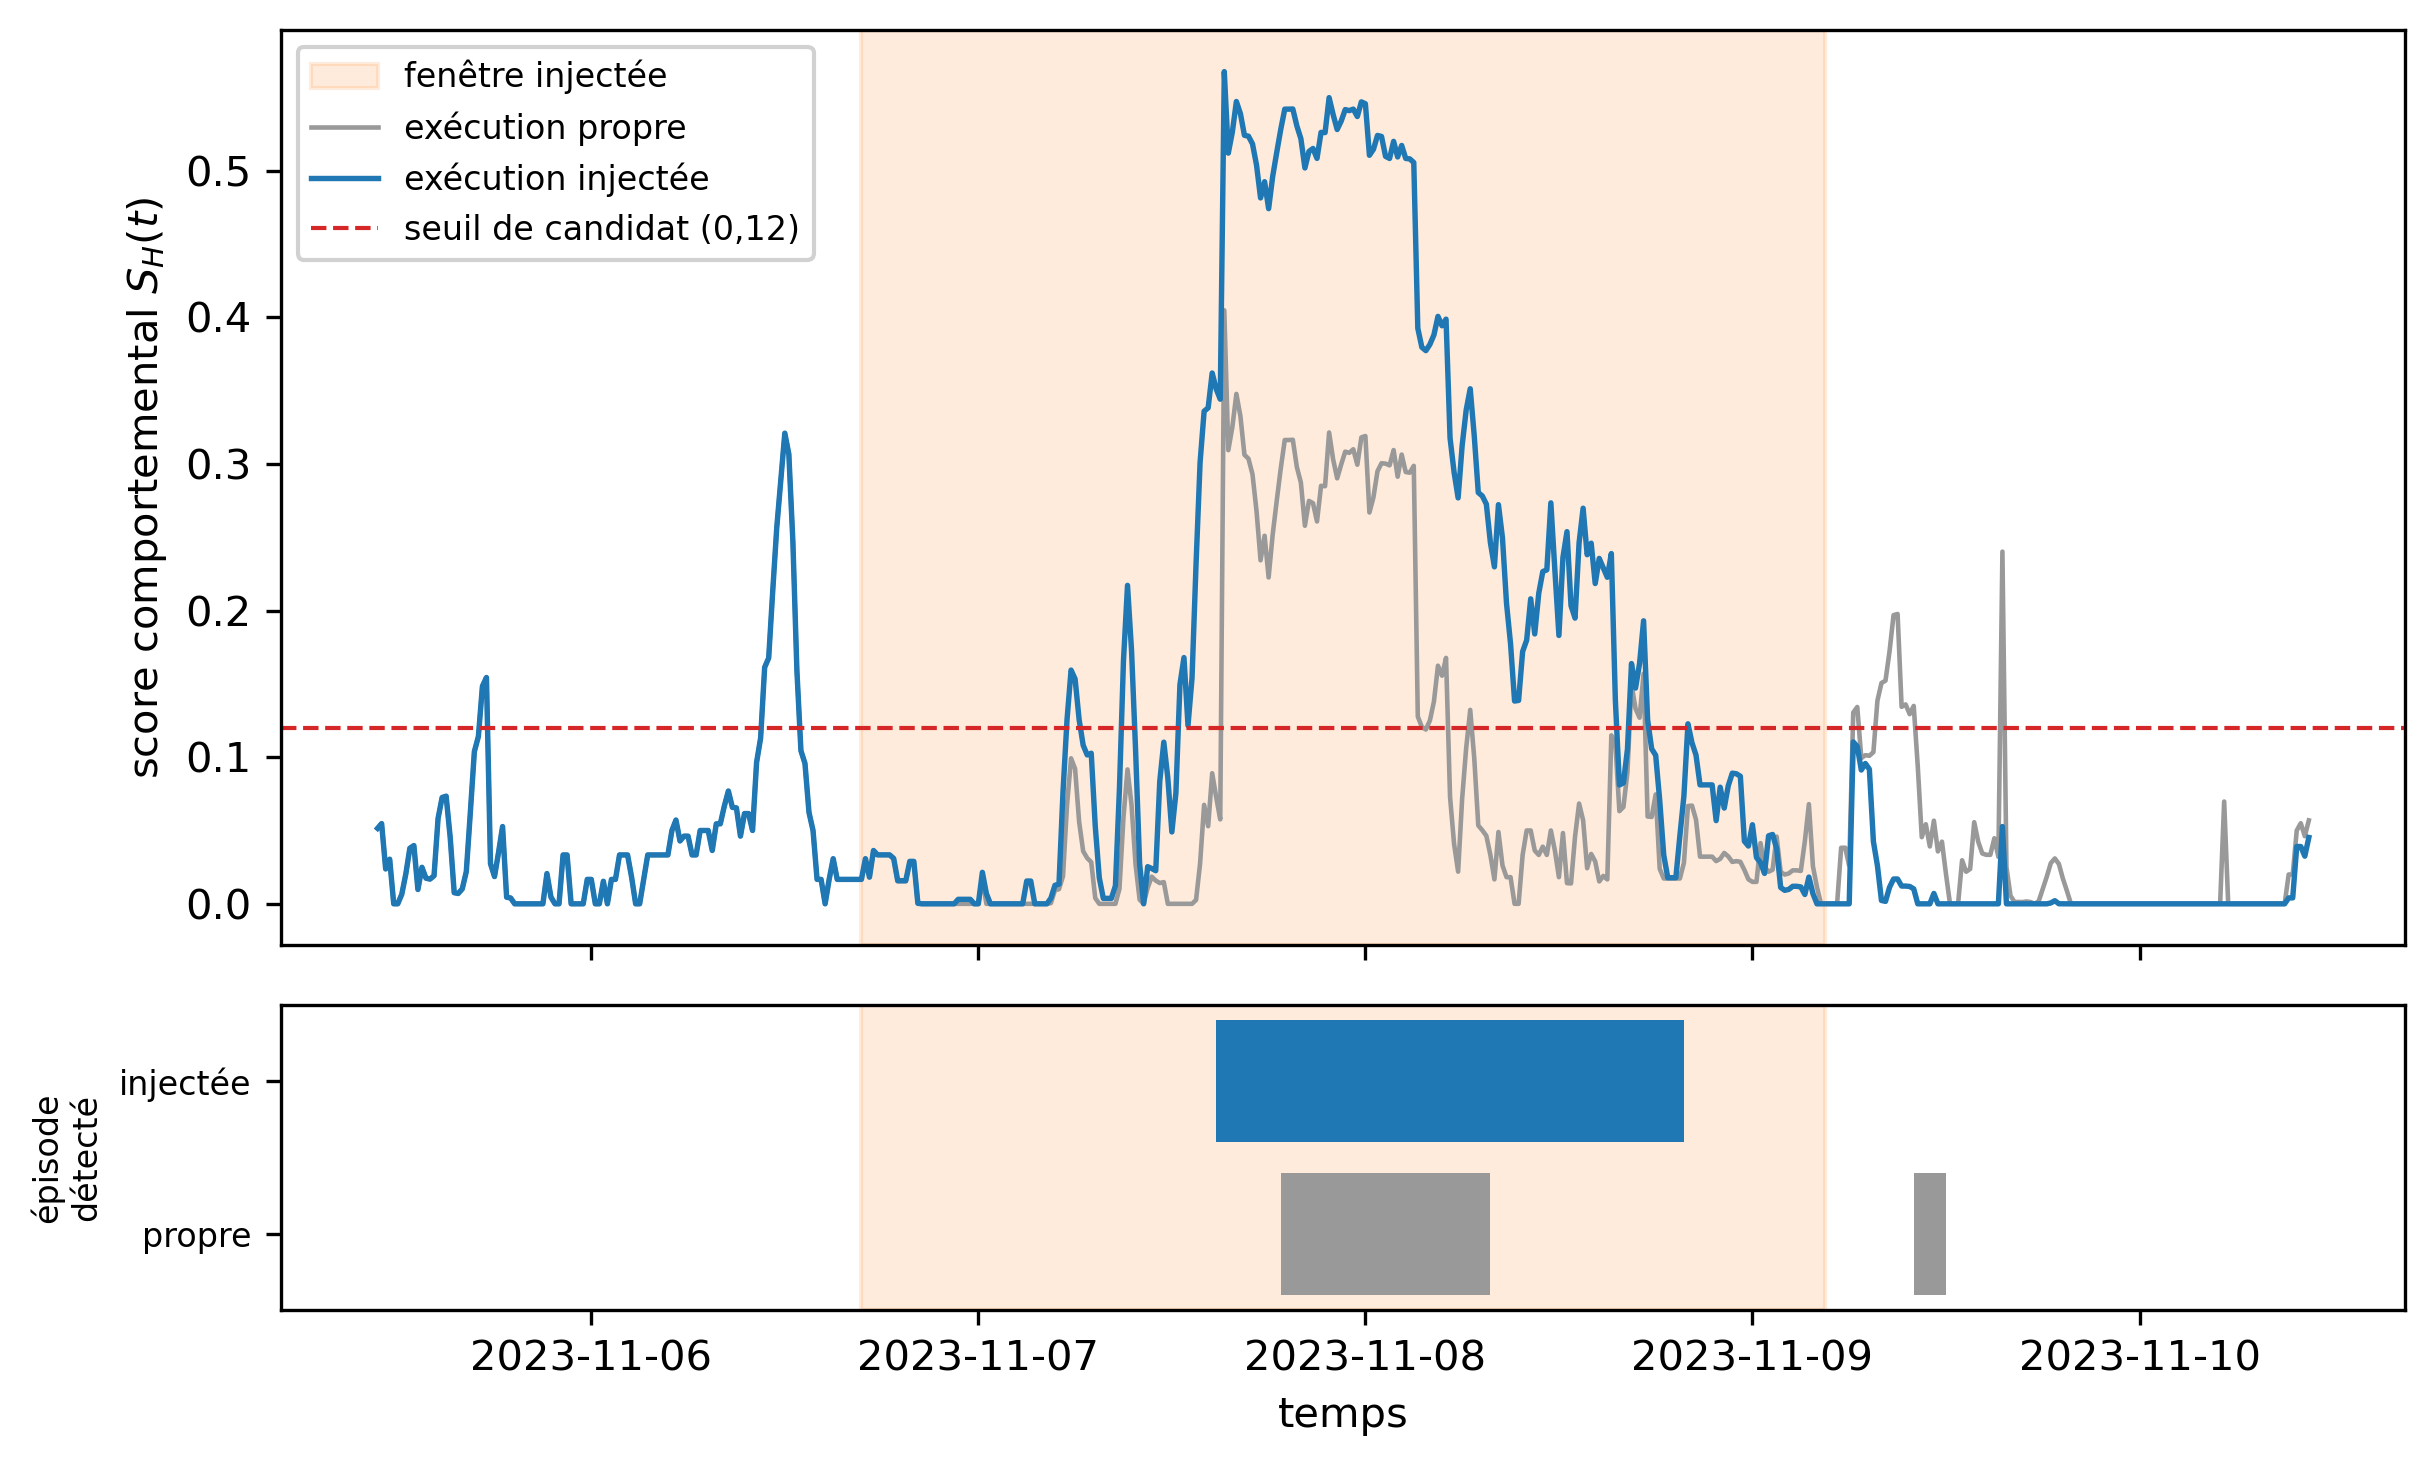
\includegraphics[width=0.95\textwidth]{figures/hypo_cusum_example.png}
  \caption{Détection attribuable au niveau de l'événement.}
  \label{fig:hypo_cusum_example}
\end{figure}

Avant tout calcul de résultat, le protocole vérifie l'unicité des identifiants d'événement,
leur non-chevauchement, leur placement strictement après la période de référence, la disponibilité des
signaux, la non-négativité des mesures, la conservation du temps postural total et l'absence
d'écriture dans le fichier source. Une campagne qui échoue à l'un de ces contrôles
n'alimente pas le manuscrit. La comparaison des fusions réutilise exactement les mêmes
vaches et les mêmes scénarios, de sorte que les écarts entre variantes ne tiennent qu'à la
règle de fusion.

% =====================================================================
\section{Métriques et analyses de sensibilité}
% =====================================================================
\subsection{Recouvrement temporel (IoU)}
La localisation d'un épisode est mesurée par l'intersection sur l'union
(\textit{Intersection over Union}, IoU), une métrique issue de la détection d'objets en
vision par ordinateur \citep{everingham2010pascal}, entre la fenêtre injectée et l'épisode
prédit~:
\begin{equation}
  \label{eq:iou}
\mathrm{IoU} = \frac{|\,\text{injecté} \cap \text{prédit}\,|}{|\,\text{injecté} \cup \text{prédit}\,|},
\end{equation}
exprimée en nombre d'intervalles de 15 minutes. Une valeur de~1 indique une superposition
parfaite, alors qu'une valeur de~0 indique une absence de chevauchement. Le seuil IoU~$\geq0{,}20$ retient
les épisodes raisonnablement localisés~; il est nettement plus strict que le simple
recouvrement, qui ne compte qu'un chevauchement non nul.

Le recours à l'IoU plutôt qu'au seul recouvrement tient à ce qu'il sanctionne les deux écarts
possibles. Un chevauchement non nul est acquis dès qu'un intervalle est partagé, quelle que
soit la durée de l'épisode prédit~: une alerte qui couvrirait toute la période surveillée
obtiendrait le même crédit qu'une alerte parfaitement ajustée. En rapportant l'intersection à
l'union, l'IoU pénalise aussi bien l'épisode trop court que l'épisode trop long. Il mesure donc
la localisation, là où le recouvrement ne mesure que la présence.

Le seuil retenu est délibérément plus bas que celui de~0,5 usuel en détection d'objets, et
deux raisons le justifient. D'une part, la fenêtre injectée possède des bornes nettes par
construction, alors qu'une dégradation comportementale réelle n'en a pas~: exiger un
recouvrement élevé reviendrait à demander au détecteur de retrouver des limites qui n'existent
que dans le protocole. D'autre part, la chaîne de détection agrège les signaux sur plusieurs
heures et impose une persistance avant de déclarer un épisode~; sa réponse est nécessairement
étalée par rapport à la fenêtre, et un seuil sévère pénaliserait le lissage qui fait sa
robustesse.

Cette métrique n'est jamais lue seule. Un IoU faible peut correspondre à une alerte qui
commence au bon moment mais se prolonge au-delà de l'événement, ce qui reste exploitable en
ferme, comme à une alerte franchement décalée, qui ne l'est pas. Les résultats la présentent
donc systématiquement à côté de la couverture attribuable et du nouveau départ~: la première
indique si le système a réagi, le second s'il a réagi par un épisode distinct de son
comportement habituel, et l'IoU indique où il a réagi.

\subsection{Métriques attribuables et unité statistique}
Une détection est attribuable seulement si l'exécution injectée ajoute un intervalle ou un
départ absent de l'exécution propre. Pour HYPO, les résultats distinguent un nouveau départ,
une couverture attribuable, un IoU~$\geq0{,}20$, le meilleur IoU, un délai et une notification
de fond. Ces entités sont volontairement reliées à des notions connues: la couverture joue le
rôle d'un rappel événementiel permissif, le nouveau départ joue le rôle d'un rappel
événementiel strict, l'IoU mesure la localisation temporelle et les notifications de fond
mesurent la charge opérationnelle. Pour
l'extension, les métriques ajoutent les taux de surveillance, de contrôle et de confusion. Les
synthèses inférentielles utilisent la vache comme unité; les lignes de 15 minutes ne sont
jamais des sujets indépendants.

Comparer les départs des deux exécutions suppose de décider quand deux départs proches sont le
même événement. Cette comparaison admet une tolérance temporelle d'une heure~: un départ de
l'exécution injectée situé à moins d'une heure d'un départ de l'exécution propre est considéré
comme le même déclenchement et n'est pas crédité. Ce choix est conservateur, et son effet est
mesuré plutôt que supposé. Sans tolérance, deux départs distants d'un seul intervalle
compteraient comme distincts et le taux de nouveau départ atteindrait 50,0\,\% au lieu de
43,2\,\%~; avec deux heures, il descendrait à 38,6\,\%. Ce balayage de la tolérance est
reproductible par un script nommé
\path{scripts/compute_match_tolerance_sensitivity.py}. La valeur retenue n'est donc pas celle
qui flatte le résultat. La couverture attribuable et l'IoU ne dépendent pas de cette décision,
puisqu'elles se calculent sur les intervalles attribuables sans jamais apparier de départs~:
elles restent inchangées sur toute la plage et servent de témoin à cette vérification.

La dépendance temporelle entre les intervalles successifs est quantifiée sur le corpus par le
temps d'autocorrélation intégré $\tau$ et par la taille d'échantillon effective
$n_{\text{eff}}=n/\tau$, où $n$ désigne le nombre d'observations disponibles et $\tau$ le temps
d'autocorrélation exprimé en nombre de pas d'échantillonnage. Les résultats descriptifs
correspondants seront présentés à la Section~\ref{subsec:statistiques_corpus}. Comme les fenêtres
glissantes voisines partagent une grande partie de leurs mesures, c'est la vache qui constitue
l'unité de rééchantillonnage. Le calcul est reproductible par un script nommé
\path{scripts/compute_correlation_time.py}.

La détection peut aussi être résumée, au niveau de l'événement, par un score F1. Les
dégradations graduelles constituent les positifs attendus, tandis que les contrôles brefs
constituent les négatifs attendus. Un vrai positif correspond à un événement graduel détecté de
façon attribuable, alors qu'un faux positif représente un contrôle bref alerté à tort. D'autre
part, un faux négatif correspond à un événement graduel manqué, tandis qu'un vrai négatif
correspond à un contrôle correctement rejeté. Le score F1 est la moyenne harmonique de la
précision et du rappel correspondants. Cela dit, cette synthèse reste complémentaire: elle
n'intègre ni la charge de fond ni la qualité fine de localisation.

\subsection{Analyses de sensibilité prévues}
L'analyse OFAT évalue
20 variantes des paramètres de HYPO, obtenues en ne modifiant qu'une valeur à la fois.
Une analyse plus restreinte modifie ensuite l'agrégation, la persistance et les seuils de la
branche INSTABILITÉ. Les deux analyses servent à détecter une dépendance excessive aux
valeurs de référence, non à optimiser les paramètres sur les événements évalués.

Deux analyses exploratoires complètent ce dispositif sans modifier la configuration
principale. La première estime, uniquement sur la période de référence de chaque vache, un facteur
proportionnel à l'écart-type de son score, puis ré-exécute la campagne avec un seuil
individualisé. La seconde fait varier le seuil de score HYPO de 0,04 à 0,20, une plage qui encadre
symétriquement la valeur retenue de 0,12, en conservant
les mêmes vaches, fenêtres, injections et autres paramètres. Elle décrit conjointement la
réponse aux événements graduels et la charge produite par les exécutions propres. Ces
analyses ont été ajoutées après la campagne principale~: elles servent à examiner des
hypothèses et non à sélectionner rétrospectivement une nouvelle valeur de seuil.

% =====================================================================
\section{Reproductibilité et organisation logicielle}
% =====================================================================
Les configurations et les sorties sont exportées en fichiers CSV. Les tests vérifient le placement
postérieur à la période de référence, la conservation posturale, la fusion et les contrats
de sortie. L'Annexe~\ref{annexe:validation} fournit les commandes de reproduction. Cette
démarche rejoint les recommandations sur la reproductibilité en apprentissage automatique et
la gestion FAIR des données \citep{pineau2021improving,wilkinson2016fair}.

\subsection{Organisation du logiciel}
Le Tableau~\ref{tab:modules} récapitule les composants logiciels et les campagnes de
reproduction qui produisent les sorties du mémoire.

\begin{table}[H]
  \centering
  \caption{Composants logiciels et campagnes de reproduction du mémoire.}
  \label{tab:modules}
  \begingroup
  \small
  \setlength{\tabcolsep}{5pt}
  \begin{tabular}{p{0.31\textwidth}p{0.62\textwidth}}
    \toprule
    Composant & Rôle \\
    \midrule
    Chargement des données & Lecture CSV, colonnes et horodatage. \\
    Dérivation des variables & Agrégation 15 min, couverture et variables dérivées. \\
    Branche HYPO & Référence individuelle, score, CUSUM et persistance. \\
    Branche INSTABILITÉ & Mouvement disproportionné, posture fragmentée et fusion. \\
    Pipeline troupeau & Orchestration par vache et agrégation troupeau. \\
    Comparateur Isolation Forest & Référence non supervisée pour l'ablation et l'interface. \\
    Évaluation HYPO & Campagne principale après la période de référence. \\
    Ablation HYPO & Comparaison avec IF, LOF et le comparateur pédométrique. \\
    Sensibilité HYPO & Analyse OFAT sans sélection de nouvelle configuration. \\
    Test de stress HYPO & Formes moins favorables à aire d'enveloppe appariée, sans nouveau réglage. \\
    Calibration par vache & Test exploratoire d'un seuil individualisé. \\
    Courbe détection-charge & Compromis entre détection attribuable et charge de fond. \\
    Évaluation bidirectionnelle & Scénarios HYPO, INSTABILITÉ, séquence et contrôles. \\
    Sensibilité de la fusion & Comparaison des règles de fusion et sensibilité technique. \\
    Analyse IceTag-SLS synchronisée & Confrontation exploratoire aux scores locomoteurs. \\
    Interface Streamlit & Visualisation individuelle, classement troupeau et export des alertes. \\
    Tests automatisés & Tests unitaires, invariants et non-régression. \\
    \bottomrule
  \end{tabular}
  \endgroup
\end{table}

Les fichiers exécutables exacts sont répartis par responsabilité: \texttt{core/} porte le
noyau de détection, soit les variables dérivées, les deux branches et leur
fusion, \texttt{validation\_hypo/} et \texttt{validation\_hybrid/} portent les
campagnes reproductibles, \texttt{scripts/} regroupe les tâches de soutien, \texttt{app.py}
et \texttt{ui/} portent l'interface, et \texttt{tests/} regroupe les contrôles automatisés.
Les scripts réutilisent les campagnes existantes sans introduire de logique d'alerte
parallèle.

\subsection{Technologies et dépendances}
Les principales dépendances sont figées dans le fichier \path{requirements.txt} et leurs
versions exactes sont reportées au Tableau~\ref{tab:technologies}, en annexe. Elles servent à
reconstruire l'environnement et à garantir la reproductibilité numérique~; elles ne constituent
pas un résultat scientifique.
Les comparateurs IF et LOF proviennent de \texttt{scikit-learn}
\citep{sklearn_api}, les tests statistiques de \texttt{SciPy} \citep{virtanen2020scipy},
et l'interface de \texttt{Streamlit}; la manipulation des données et le calcul numérique
reposent sur \texttt{pandas} \citep{mckinney2010data} et \texttt{NumPy} \citep{harris2020array}.


\subsection{Évaluation du temps d'exécution}
L'évaluation reconstruit les variables, exécute le comparateur Isolation Forest, les règles
IF comparatives, HYPO, INSTABILITÉ et la fusion hiérarchique. Chaque étape est chronométrée avec
une horloge monotone. Cinq répétitions sont effectuées sur l'ensemble du corpus principal et la concaténation
des sorties intervalle est incluse. Le résultat canonique est la médiane des cinq durées; les
valeurs minimale et maximale sont conservées pour rendre visible la variabilité de la machine.
Cette évaluation du temps d'exécution documente la faisabilité du prototype sur l'ordinateur
utilisé, non un temps garanti en production.

\subsection{Tests et traçabilité}
La suite automatisée contient 136 tests et couvre le chargement, les variables dérivées,
les deux détecteurs, les valeurs de référence du Tableau~\ref{tab:config_finale}, les cinq fusions
et l'asymétrie de la règle hiérarchique, les injections, les contrôles après la période de référence,
l'isolement de la période de référence vis-à-vis de la période future et le caractère unilatéral du cumul,
l'appariement de l'aire d'enveloppe, l'analyse de sensibilité, l'analyse SLS exacte et le démarrage de
Streamlit. Les résultats sont
écrits dans des fichiers tabulaires dont la provenance est explicite. Le succès des tests
atteste la cohérence logicielle et sécurise la reproduction des résultats.

Chaque résultat suit un cycle de vie traçable en trois étapes~: 1-~une commande de
reproduction exécute un module d'évaluation, qui écrit des fichiers CSV et JSON~; 2-~un
manifeste SHA-256 fige ces sorties ainsi que l'empreinte du corpus confidentiel~; 3-~un
script dédié les transforme automatiquement en figures de résultats du manuscrit. Aucun résultat empirique n'est accepté sans comparaison
à son artefact source. Une modification du code, des données ou des paramètres impose donc
une nouvelle exécution et un nouveau manifeste, de sorte que le PDF du mémoire ne constitue jamais
à lui seul la trace de référence de l'expérience. La Figure~\ref{fig:repro_chain} illustre cette chaîne de reproductibilité.

\begin{figure}[H]
  \centering
  \begin{tikzpicture}[
    procbox/.style={rectangle, draw=black!55, rounded corners=2pt, align=center,
      minimum height=1.55cm, text width=2.15cm, font=\normalsize, inner sep=4pt},
    arrow/.style={-{Stealth[length=2.4mm, width=1.6mm]}, line width=0.8pt, black!65}]
    \node[procbox, fill=profgray!10] (csv) at (0,0)
      {\textbf{1}\\Données IceQube};
    \node[procbox, fill=ifblue!10] (split) at (3.0,0)
      {\textbf{2}\\Séparation temporelle};
    \node[procbox, fill=loforange!10] (inject) at (6.0,0)
      {\textbf{3}\\Injection future};
    \node[procbox, fill=rulegreen!12] (detect) at (9.0,0)
      {\textbf{4}\\HYPO et fusion};
    \node[procbox, fill=ifblue!8] (attrib) at (12.0,0)
      {\textbf{5}\\Attribution des sorties};
    \node[procbox, fill=profgray!10] (out) at (12.0,-2.35)
      {\textbf{6}\\Résultats CSV};
    \node[procbox, fill=profgray!10] (fig) at (9.0,-2.35)
      {\textbf{7}\\Figures du mémoire};
    \node[procbox, fill=rawred!12] (sha) at (6.0,-2.35)
      {\textbf{8}\\Manifeste SHA-256};
    \draw[arrow] (csv) -- (split);
    \draw[arrow] (split) -- (inject);
    \draw[arrow] (inject) -- (detect);
    \draw[arrow] (detect) -- (attrib);
    \draw[arrow] (attrib) -- (out);
    \draw[arrow] (out) -- (fig);
    \draw[arrow] (fig) -- (sha);
  \end{tikzpicture}
  \caption{Chaîne de reproductibilité, des données brutes au manifeste SHA-256.}
  \label{fig:repro_chain}
\end{figure}

Le manifeste ferme la chaîne en rendant toute modification d'un artefact détectable. Il
atteste l'identité des fichiers reproduits et complète les contrôles méthodologiques décrits
dans le chapitre des résultats.

\chapter{Données et cadre expérimental}
\label{chapitre:donnees}

Ce chapitre décrit les données sur lesquelles le système est évalué, puis le cadre
expérimental correspondant. Il présente le corpus principal IceQube 2023, sa préparation et
ses variables dérivées, avant de détailler les campagnes injectées et la cohorte
IceTag-SLS.

% =====================================================================
\section{Corpus principal IceQube 2023}
% =====================================================================
\label{sec:donnees}

Le fichier \texttt{data/brut.csv} provient de la ferme du campus Macdonald de
l'Université McGill. Il contient 37\,839 mesures de 28 vaches entre le
1\textsuperscript{er} octobre et le 11 novembre 2023. Les variables sont agrégées à une
résolution nominale de 15 minutes. Le Tableau~\ref{tab:dataset} en décrit les
caractéristiques vérifiées.

\begin{table}[H]
  \centering
  \caption{Caractéristiques vérifiées du corpus IceQube 2023.}
  \label{tab:dataset}
  \small
  \begin{tabular}{lr}
    \toprule
    Caractéristique & Valeur \\
    \midrule
    Vaches & 28 \\
    Lignes & 37\,839 \\
    Résolution nominale & 15 minutes \\
    Période & 1 octobre--11 novembre 2023 \\
    Lignes par vache, médiane & 564 \\
    Lignes par vache, étendue & 244--2\,474 \\
    Doublons vache-temps & 0 \\
    \bottomrule
  \end{tabular}
\end{table}

\subsection{Variables brutes du corpus}
Les variables utilisées sont les pas, le \textit{Motion Index}, le temps couché, le temps
debout, les transitions et leur décomposition en levers et couchers
(Tableau~\ref{tab:variables_brutes}). Elles décrivent la quantité de mouvement et la
posture, contrairement à la mesure de l'asymétrie de démarche, de la douleur ou des lésions
du pied \citep{alsaaod2019automatic,oleary2020accelerometers}. Leur portée clinique est donc
indirecte.

\begin{table}[H]
  \centering
  \caption{Variables brutes du corpus IceQube 2023.}
  \label{tab:variables_brutes}
  \small
  \begin{tabular}{p{0.28\textwidth}p{0.60\textwidth}}
    \toprule
    Variable & Interprétation \\
    \midrule
    \textit{Steps} & Nombre de pas dans l'intervalle. \\
    \textit{Motion Index} & Intensité agrégée du mouvement mesuré par le capteur. \\
    \textit{Lying Time} & Temps couché dans l'intervalle. \\
    \textit{Standing Time} & Temps debout dans l'intervalle. \\
    \textit{Transitions} & Nombre total de transitions posturales. \\
    \textit{Transitions Up/Down} & Décomposition en levers et couchers. \\
    \bottomrule
  \end{tabular}
\end{table}

\subsection{Statistiques descriptives et variabilité inter-individuelle}
\label{subsec:statistiques_corpus}
Les distributions sont fortement asymétriques, comme le montre le
Tableau~\ref{tab:statistiques_brutes}~: la médiane des pas et des transitions par intervalle est nulle, tandis que les maxima sont
élevés. Cette structure écarte une normalisation gaussienne globale et motive des
comparaisons robustes propres à chaque vache et à chaque créneau horaire
\citep{leys2013detecting}.

\begin{table}[H]
  \centering
  \caption{Statistiques descriptives des variables de mouvement (par intervalle de 15~min).}
  \label{tab:statistiques_brutes}
  \small
  \begin{tabular}{lrrrr}
    \toprule
    Variable & Moyenne & Écart-type & Médiane & Maximum \\
    \midrule
    Pas & 4,0 & 15,4 & 0 & 387 \\
    \textit{Motion Index} & 25,5 & 103,7 & 5 & 3\,351 \\
    Transitions & 0,16 & 0,40 & 0 & 6 \\
    \bottomrule
  \end{tabular}
\end{table}

L'autocorrélation confirme que les intervalles successifs ne constituent pas des observations
indépendantes. Après mise sur une grille régulière et déduplication temporelle par vache, les
36\,879 mesures exploitables correspondent à environ 10\,000 observations indépendantes pour
le \textit{Motion Index}; au grain brut de 15 minutes, le temps d'autocorrélation intégré
est de l'ordre d'une heure pour les signaux d'activité. Au niveau de décision, les totaux
glissants de 12 heures portent ce temps à environ huit heures~: la médiane par vache tombe
alors à environ 17 points de décision indépendants. Les séries étant très inégales, cette
médiane ne se multiplie pas par l'effectif~; la somme des tailles effectives reste néanmoins de
l'ordre du millier sur l'ensemble du corpus, soit 1\,151 points pour les pas et 880 pour le
\textit{Motion Index}. Ce résultat justifie l'agrégation statistique par vache et le
rééchantillonnage groupé employés dans l'évaluation; il évite que la dépendance entre
intervalles produise des intervalles de confiance artificiellement étroits.

La variabilité entre vaches est considérable, comme le montre le
Tableau~\ref{tab:variabilite}. La moyenne de
pas par intervalle varie de 0,0 à 11,1 selon la vache, et le coefficient de variation
inter-vache atteint 0,50 pour les pas, 0,40 pour le \textit{Motion Index} et 0,41 pour les
transitions. Cette hétérogénéité interdit un seuil commun à tout le troupeau et justifie le
recours à une référence \emph{individuelle}, propre à chaque vache.

\begin{table}[H]
  \centering
  \caption{Variabilité inter-individuelle des principales variables (moyenne par vache).}
  \label{tab:variabilite}
  \small
  \begin{tabular}{lrrr}
    \toprule
    Variable & Moyenne/vache min & Moyenne/vache max & CV inter-vache \\
    \midrule
    Pas & 0,0 & 11,1 & 0,50 \\
    \textit{Motion Index} & 4,0 & 57,4 & 0,40 \\
    Transitions & 0,00 & 0,31 & 0,41 \\
    \bottomrule
  \end{tabular}
\end{table}

% =====================================================================
\section{Préparation des données et variables dérivées}
% =====================================================================
Cette section décrit les traitements appliqués aux mesures brutes avant la détection~: le
choix de la résolution, les contrôles d'admissibilité, la traçabilité des fichiers et la
construction des variables dérivées.

\subsection{Résolution temporelle}
\label{sec:resolution_temporelle}
L'agrégation à 15 minutes est conservée comme résolution nominale. Une résolution plus
fine multiplie le bruit et les intervalles vides sans ajouter d'information comportementale
exploitable à l'échelle d'un épisode de plusieurs heures~; une résolution plus grossière
masque les transitions posturales. Une résolution de 15 minutes permet d'avoir un compromis entre stabilité du
signal et granularité suffisante pour la persistance recherchée par les deux branches.

\subsection{Contrôles d'admissibilité}
Le chargement impose des dates interprétables, des identifiants non vides et des variables
numériques non négatives~; les durées posturales sont converties en minutes et la couverture
de chaque intervalle est conservée. Les données originales ne sont jamais modifiées par
l'évaluation~: chaque injection opère sur une copie en mémoire.

Le corpus regroupe 16 vaches suivies pendant moins de 14 jours et 12 vaches disposant de
séries plus longues. Pour être admissible à l'évaluation synthétique, une vache doit disposer
d'au moins 14 jours de mesures, d'une période future après la période de référence et de
valeurs informatives pour les pas, le \textit{Motion Index} et les transitions. Ces critères
retiennent 11 vaches. Les 28 vaches demeurent néanmoins disponibles dans l'interface~; la
restriction à 11 animaux s'applique uniquement au protocole expérimental.

La Figure~\ref{fig:admissibilite} présente les identifiants des vaches sur l'axe vertical et la
durée des séries sur l'axe horizontal. Les 11 vaches admissibles sont représentées en vert et
les 17 vaches non admissibles en gris. Le trait pointillé représente le seuil de 14 jours.
Parmi les vaches non admissibles, 16 se trouvent sous ce seuil. La vache 8144 le dépasse,
mais ses signaux ne sont pas informatifs dans la période future, ce qui explique son exclusion.

\begin{figure}[H]
  \centering
  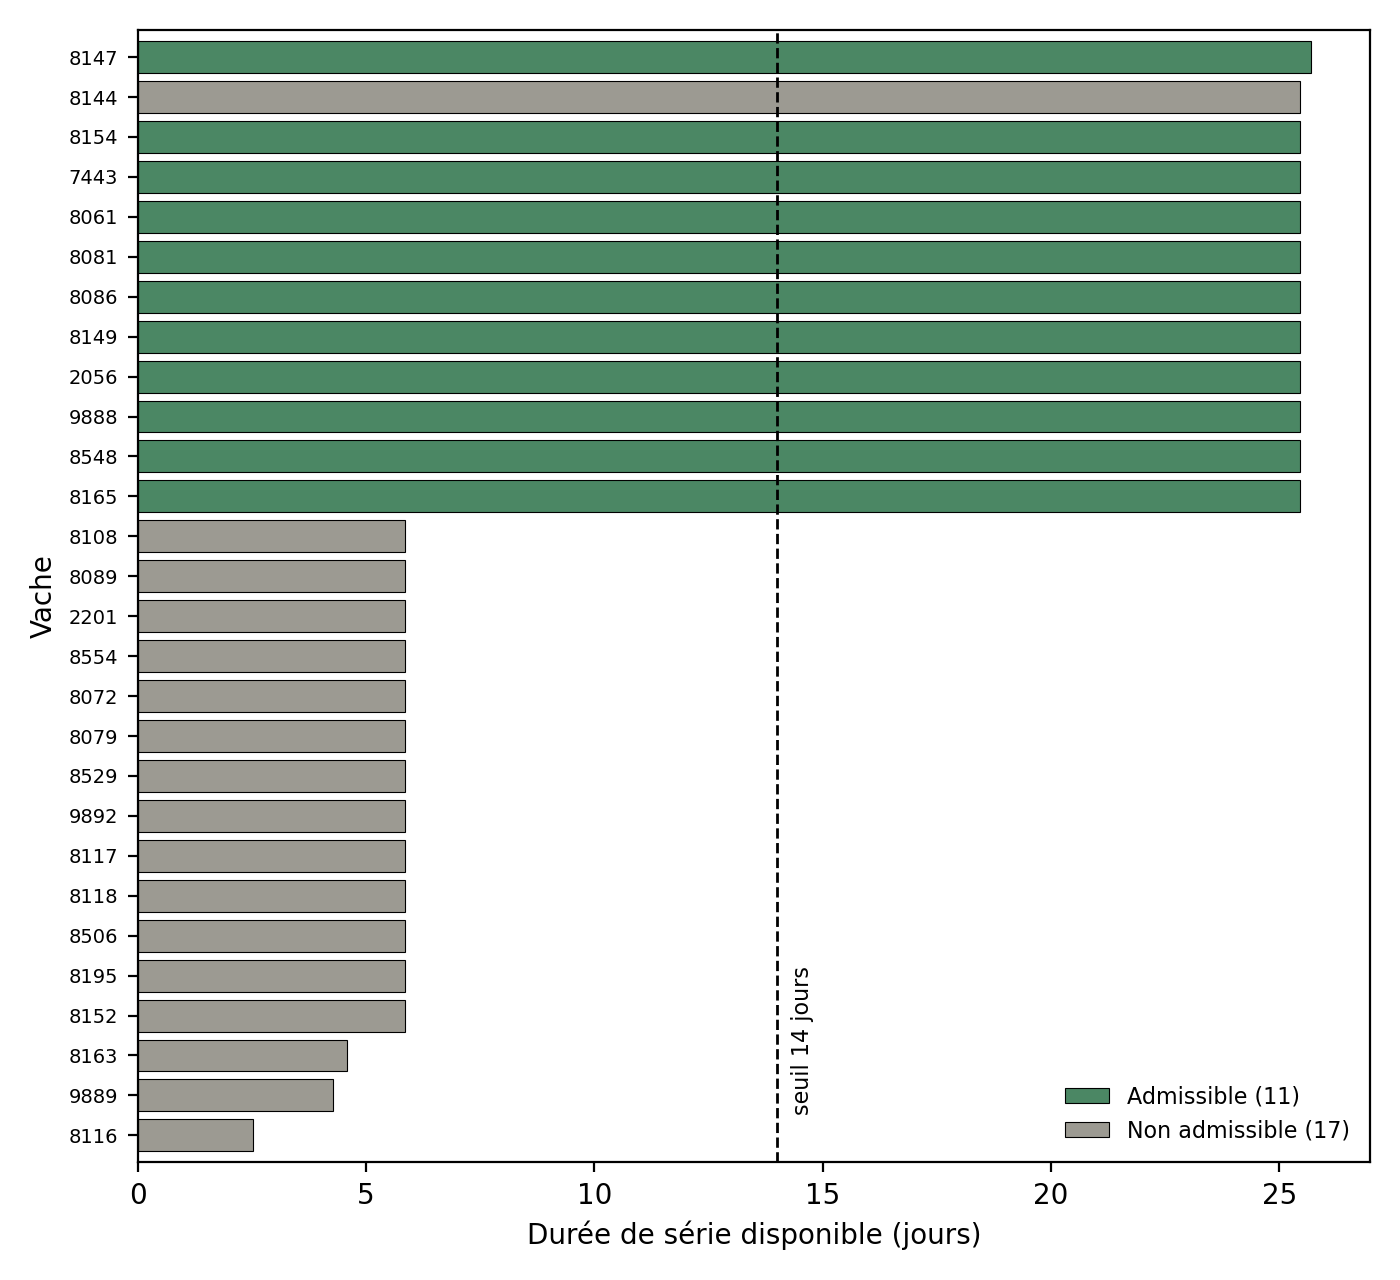
\includegraphics[width=0.80\textwidth]{figures/cow_admissibility.png}
  \caption{Admissibilité des vaches.}
  \label{fig:admissibilite}
\end{figure}

\subsection{Traçabilité et provenance des données}
La provenance du corpus a été vérifiée en confrontant ses valeurs à celles du système
commercial CowAlert (IceRobotics), qui restitue les mêmes mesures IceQube
\citep{icerobotics2012cowalert}. Pour les 5 vaches dont les mesures ont pu être relevées
depuis ce système, les deux sources de données, soit le corpus brut et l'export CowAlert,
sont alignées sur la clé vache-début d'intervalle, après vérification de l'absence de
doublons. Les 7\,631 intervalles communs représentent 97,5\,\% des 7\,823 lignes de
l'export CowAlert. Pour ces intervalles, les pas, le \textit{Motion Index} et les
transitions sont identiques, avec une corrélation parfaite de 1,0. Le corpus correspond
donc aux mesures restituées par le système officiel pour ces vaches. À noter que cette
vérification porte sur 5 des 28 vaches. Seules les corrélations agrégées sont rapportées,
puisque l'export CowAlert est confidentiel.

\subsection{Variables dérivées}
La chaîne de traitement calcule plusieurs variables dérivées à partir de chaque variable
brute, comme le montre le Tableau~\ref{tab:features}. Elle produit des agrégats par intervalle,
des transformations logarithmiques qui atténuent l'asymétrie, des z-scores robustes globaux
et glissants, ainsi qu'un indicateur de couverture. Ces variables alimentent IF, LOF et les
règles de cohérence qui leur sont associées. HYPO et INSTABILITÉ utilisent plutôt des ratios
calculés par rapport à la référence individuelle.

\begin{table}[H]
  \centering
  \caption{Familles de variables dérivées par variable comportementale brute.}
  \label{tab:features}
  \small
  \begin{tabular}{p{0.32\textwidth}p{0.56\textwidth}}
    \toprule
    Famille & Description \\
    \midrule
    Agrégats & Somme et moyenne par intervalle de 15 minutes. \\
    Transformations log & $\log(1+x)$ sur la somme et la moyenne. \\
    Z-score robuste global & Centrage par la médiane, échelle par l'écart absolu médian (MAD). \\
    Z-score robuste glissant & Même principe sur une fenêtre mobile de 24~intervalles. \\
    Couverture & Rapport entre échantillons observés et attendus par intervalle. \\
    \bottomrule
  \end{tabular}
\end{table}

% =====================================================================
\section{Cadre expérimental}
\label{sec:cadre_experimental}
% =====================================================================
Le cadre expérimental comprend deux campagnes injectées principales, une campagne de stress
complémentaire et une cohorte observationnelle distincte. La
Figure~\ref{fig:plan_etude} présente cette organisation.

\begin{figure}[H]
  \centering
  \begin{tikzpicture}[
    box/.style={rectangle, draw=black!55, rounded corners=2pt, align=center,
      minimum height=2.1cm, minimum width=3.7cm, text width=3.4cm, inner sep=6pt, font=\small},
    arrow/.style={-{Stealth[length=2.2mm]}, thick, black!65}]
    \node[box, fill=ifblue!10] (main) {IceQube 2023\\28 vaches};
    \node[box, fill=rulegreen!10, right=0.4cm of main] (split) {Référence 60\,\%\\futur 40\,\%};
    \node[box, fill=loforange!10, right=0.4cm of split] (inject) {HYPO: 44\\INSTABILITÉ: 132\\stress: 198};
    \node[box, fill=profgray!10, right=0.4cm of inject] (eval) {Comparaison propre-injectée\\unité: vache};
    \draw[arrow] (main) -- (split); \draw[arrow] (split) -- (inject); \draw[arrow] (inject) -- (eval);
    \node[box, fill=ifblue!7, below=0.8cm of main] (sls) {IceTag-SLS 2019\\14 vaches};
    \node[box, fill=rulegreen!7, below=0.8cm of split] (pre) {Sept jours\\avant le SLS};
    \node[box, fill=profgray!7, below=0.8cm of inject] (conc) {Concordance exploratoire\\sans réglage};
    \draw[arrow] (sls) -- (pre); \draw[arrow] (pre) -- (conc);
  \end{tikzpicture}
  \caption{Plan d'étude.}
  \label{fig:plan_etude}
\end{figure}

Les trois niveaux présentés sont les suivants~:
\begin{itemize}
  \item le premier niveau évalue HYPO sur 44 événements et le compare aux trois variantes
  fondées sur IF ou LOF ainsi qu'au comparateur pédométrique;
  \item le deuxième niveau applique 132 scénarios afin d'explorer INSTABILITÉ et cinq règles
  de fusion;
  \item le troisième niveau analyse une cohorte IceTag-SLS de l'hiver 2019 composée de
  14 vaches. Il utilise les mesures des sept jours précédant le score locomoteur et ne sert
  pas à régler le système.
\end{itemize}

Dans chacun des deux premiers niveaux, un scénario est injecté dans une copie distincte de la
période future, puis comparé à l'exécution propre de la même vache. Ce plan forme un banc
d'essai contrefactuel reproductible~: l'événement synthétique est le seul changement
volontaire entre l'exécution propre et l'exécution injectée, ce qui permet de mesurer la
réponse du détecteur sans modifier la période de référence ni optimiser les seuils sur les
sorties observées.

Une campagne de stress complémentaire réexécute aussi HYPO et les quatre comparateurs sur
six formes moins favorables, à trois positions par vache. Elle est séparée des résultats qui
ont servi à construire le système. Son protocole JSON interdit tout nouveau réglage et
apparie l'aire de l'enveloppe numérique~: pour chaque famille modifiée, l'aire discrète sous
l'enveloppe, calculée sur les intervalles effectivement conservés, est égale à celle du
profil modéré graduel de 48 heures. Cette contrainte évite d'attribuer à la forme temporelle
un effet qui proviendrait seulement d'une enveloppe programmée plus intense; elle ne garantit
pas une amplitude physiologique ou comportementale identique. Le contrôle négatif modifie
uniquement les pas avec la même aire numérique; le scénario de données manquantes retire un
bloc contigu de 12 heures après cet appariement.

\subsection{Campagne principale et ablation du module HYPO}
La campagne principale construit quatre événements pour chacune des 11 vaches admissibles,
soit 44 événements~:
\begin{itemize}
  \item le profil \textbf{léger} diminue progressivement les pas, le mouvement et les
  transitions, puis transfère une part du temps debout vers le temps couché pendant 36 heures;
  \item le profil \textbf{modéré} applique la même évolution pendant 48 heures;
  \item le profil \textbf{marqué} l'applique pendant 60 heures;
  \item le contrôle bref dure trois heures et ne devrait pas former un épisode persistant.
\end{itemize}
Cette campagne reprend le cadre contrefactuel de la Section~\ref{sec:cadre_experimental}.
Pour HYPO, l'exécution propre de la même vache est soustraite lors du calcul des métriques
attribuables.

L'étude d'ablation évalue l'apport de la structure temporelle et multivariée de HYPO en la
comparant à quatre configurations simplifiées ou alternatives. Les cinq variantes sont
appliquées aux mêmes fenêtres~:
\begin{itemize}
  \item (A) HYPO temporel multivarié;
  \item (B) IF suivi des règles de persistance;
  \item (C) IF ponctuel;
  \item (D) LOF suivi des règles;
  \item (E) un comparateur pédométrique restreint au seul canal des pas.
\end{itemize}
Les comparaisons appariées sont calculées après agrégation par vache. Une analyse OFAT
conserve les mêmes 11 vaches, les mêmes fenêtres et la même graine, puis modifie séparément
dix paramètres autour de la référence. Elle évalue une robustesse locale et ne sélectionne
pas une nouvelle configuration.

\subsection{Extension bidirectionnelle et contrôles de confusion}
Douze scénarios sont appliqués à chacune des onze vaches admissibles, soit 132 événements,
selon le même cadre contrefactuel. L'enveloppe est progressive, avec montée, plateau et
retour, et la somme des temps couché et debout est conservée. Le
Tableau~\ref{tab:profils_detection} décrit ces douze scénarios.

\begin{table}[H]
  \centering
  \caption{Scénarios de l'évaluation technique.}
  \label{tab:profils_detection}
  \small
  \begin{tabular}{p{0.27\textwidth}p{0.18\textwidth}p{0.43\textwidth}}
    \toprule
    Famille & Nombre & Rôle \\
    \midrule
    Hypoactivité légère, modérée, marquée & 33 & Baisse progressive de plusieurs signaux sur 24 à 48 h. \\
    Instabilité légère, modérée, marquée & 33 & Mouvement relatif, transitions et posture sur 8 à 16 h. \\
    Instabilité puis hypoactivité & 11 & Séquence séparée par 24 h. \\
    Pic capteur, exercice bref, manipulation & 33 & Contrôles brefs qui doivent être rejetés. \\
    Activité de type œstrus & 11 & Confondant d'hyperactivité coordonnée. \\
    Hypoactivité non locomotrice & 11 & Confondant causal indiscernable avec les capteurs seuls. \\
    \bottomrule
  \end{tabular}
\end{table}

L'amplitude modérée des pas atteint 29\,\%, valeur ancrée sur un ordre de grandeur publié
autour d'un parage thérapeutique \citep{paudyal2021lying}. Les amplitudes des autres signaux
sont des hypothèses de test et non des estimations cliniques.

\subsection{Cohorte IceTag-SLS de l'hiver 2019}
\label{subsec:corpus_mcgill}

Le développement et l'évaluation technique du système ont d'abord été réalisés sur le corpus
IceQube 2023. La cohorte IceTag-SLS 2019, devenue accessible dans un second temps, a ensuite
été exploitée sans modifier la configuration ni les seuils du détecteur.

Les deux ensembles de données ne sont ni fusionnés ni appariés animal par animal. Le corpus
IceQube 2023 sert à l'évaluation technique du système, tandis que la cohorte IceTag-SLS 2019
fournit une confrontation observationnelle distincte avec des scores locomoteurs contemporains.
Cette cohorte provient du même campus, mais d'une période et d'un dispositif différents.
Le SLS représente la somme de quatre composantes binaires et varie de 0 à 4. L'analyse retient le
score du 12 mars 2019 et les données capteurs strictement antérieures. Une vache doit avoir
une période de référence suffisante et au moins 70\,\% de couverture dans les sept jours précédents.
Quatorze vaches sont évaluables: deux ont un SLS de 0, neuf un SLS de 1 et trois un SLS de 2.
Aucun SLS de 3 ou 4 n'est observé. Le seuil SLS~$\geq2$ constitue une séparation
exploratoire, non un diagnostic imposé par le protocole source.

\subsection{Protocole de l'analyse SLS}
La configuration hiérarchique est appliquée sans utiliser les scores pour entraîner le
détecteur ou régler ses seuils. Dans l'analyse finale, cette fusion et le nombre de notifications
dans les sept jours précédant le 12 mars 2019 sont retenus comme analyse principale. Sont également
rapportées la fraction du temps en épisode, la surveillance d'instabilité et le score
maximum. Les comparaisons utilisent l'AUC descriptive, le test de Mann-Whitney et la
corrélation de Spearman au niveau de la vache. Avec seulement trois SLS~$\geq2$, ces mesures
restent exploratoires. Pour tenir compte exactement du petit effectif et des ex æquo, toutes
les répartitions possibles des trois étiquettes positives parmi les quatorze vaches sont
énumérées pour l'AUC. L'analyse est ensuite répétée dans le seul groupe
\textit{Exercise}; le groupe sans exercice ne contient aucun SLS~$\geq2$ et son AUC n'est
donc pas estimable. Un test exact de Fisher quantifie l'association entre traitement et
classe SLS, et une analyse leave-one-positive-out vérifie l'influence de chacune des trois
vaches positives. Enfin, une analyse de sensibilité ajoutée après l'analyse principale emploie
un test exact max-stat pour contrôler la recherche parmi les cinq variantes de fusion pour le
nombre de notifications, puis parmi les vingt combinaisons formées par les cinq variantes et
les quatre métriques. Son caractère postérieur impose une portée exploratoire; la valeur $p$
globale non ajustée est conservée comme résultat descriptif.

\chapter{Interface et valorisation opérationnelle}
\label{chapitre:interface}

L'interface de priorisation occupe ce chapitre. Le besoin opérationnel et les principes de
conception qui en découlent ouvrent l'exposé, suivis du tableau de bord et de ses trois
échelles de lecture. Les niveaux de priorité et l'action associée viennent ensuite, puis
l'export et la traçabilité des alertes, avant la portée et les limites de cet usage.

% =====================================================================
\section{Besoin opérationnel et principes de conception}
% =====================================================================
Comme précédemment mentionné au Chapitre~\ref{chapitre:contexte}, l'observation humaine
reste la référence du repérage de la boiterie, mais elle est difficile
à maintenir de façon régulière sur l'ensemble d'un troupeau, par le temps qu'elle demande et
par la variabilité entre observateurs. Les branches de détection
décrites au Chapitre~\ref{chapitre:systeme} produisent un score, des épisodes et des
notifications. Sous cette formule, ces sorties répondent
à la question « que dit le détecteur~? », alors que la question de terrain est la suivante~:
« quelles vaches dois-je aller voir aujourd'hui, et pourquoi~? ». L'interface graphique
proposée comble cet écart en transformant des séries de sortie en une liste ordonnée de
vaches à vérifier. Sa conception suit quatre principes, qui découlent du positionnement
retenu pour le système.
\begin{itemize}
  \item \emph{La priorisation plutôt que le diagnostic}. L'interface ordonne les
  vaches à observer, sans quantifier réellement une probabilité de boiterie ou afficher un
  libellé clinique. Cette contrainte est délibérée~: le corpus principal ne comporte pas
  d'étalon vétérinaire, et un affichage qui suggérerait une conclusion clinique dépasserait ce
  que les données autorisent \citep{alsaaod2019automatic}.

  \item \emph{La traçabilité de chaque alerte}. La vue individuelle présente les
  signaux, les épisodes et les notifications d'une même vache, de sorte qu'une priorité
  affichée peut toujours être remontée jusqu'aux mesures qui l'ont produite. Une alerte
  opaque serait inutilisable en ferme. L'éleveur doit alors pouvoir juger lui-même si le
  comportement observé justifie un déplacement.

  \item \emph{La séparation entre surveillance et vérification}. Une instabilité
  isolée n'appelle pas le même geste qu'une hypoactivité persistante. L'interface conserve
  cette distinction au lieu de fondre les deux branches en un signal similaire, ce qui évite de
  transformer une piste exploratoire en consigne de travail.

  \item \emph{L'absence de logique d'alerte parallèle}. L'interface lit les sorties
  du noyau de détection et ne recalcule aucune règle qui lui serait propre. Une modification de
  présentation ne peut donc pas changer silencieusement les résultats rapportés
  \citep{sculley2015hidden}.
\end{itemize}

% =====================================================================
\section{Tableau de bord de priorisation}
\label{sec:interface_streamlit}
% =====================================================================
L'interface proposée est un outil de lecture et de priorisation. Elle charge par défaut le
fichier d'entrée \texttt{data/brut.csv} et accepte un CSV importé
(Figure~\ref{fig:streamlit_overview}). La vue troupeau ordonne
les vaches à vérifier tandis que la carte thermique permet une comparaison journalière. La
méthode IF est toujours sollicitée comme comparateur qui ne constitue pas la notification
principale.

La barre latérale regroupe le chargement des données et les paramètres de calcul, tandis que
l'en-tête rappelle la source analysée, son volume et son empreinte. Les six compteurs
résument, pour la vache sélectionnée, le nombre d'intervalles analysés puis fusionnés, les
anomalies du comparateur, les candidats de chaque branche et les notifications retenues.

\begin{figure}[H]
  \centering
  % La capture fait 2878 px de large : a 0,98 de la largeur du texte, soit
  % 6,40 pouces, elle rend a 450 ppp, tres au-dessus du seuil d'impression. Le
  % rapport large et bas de la vue tient en une demi-page en portrait.
  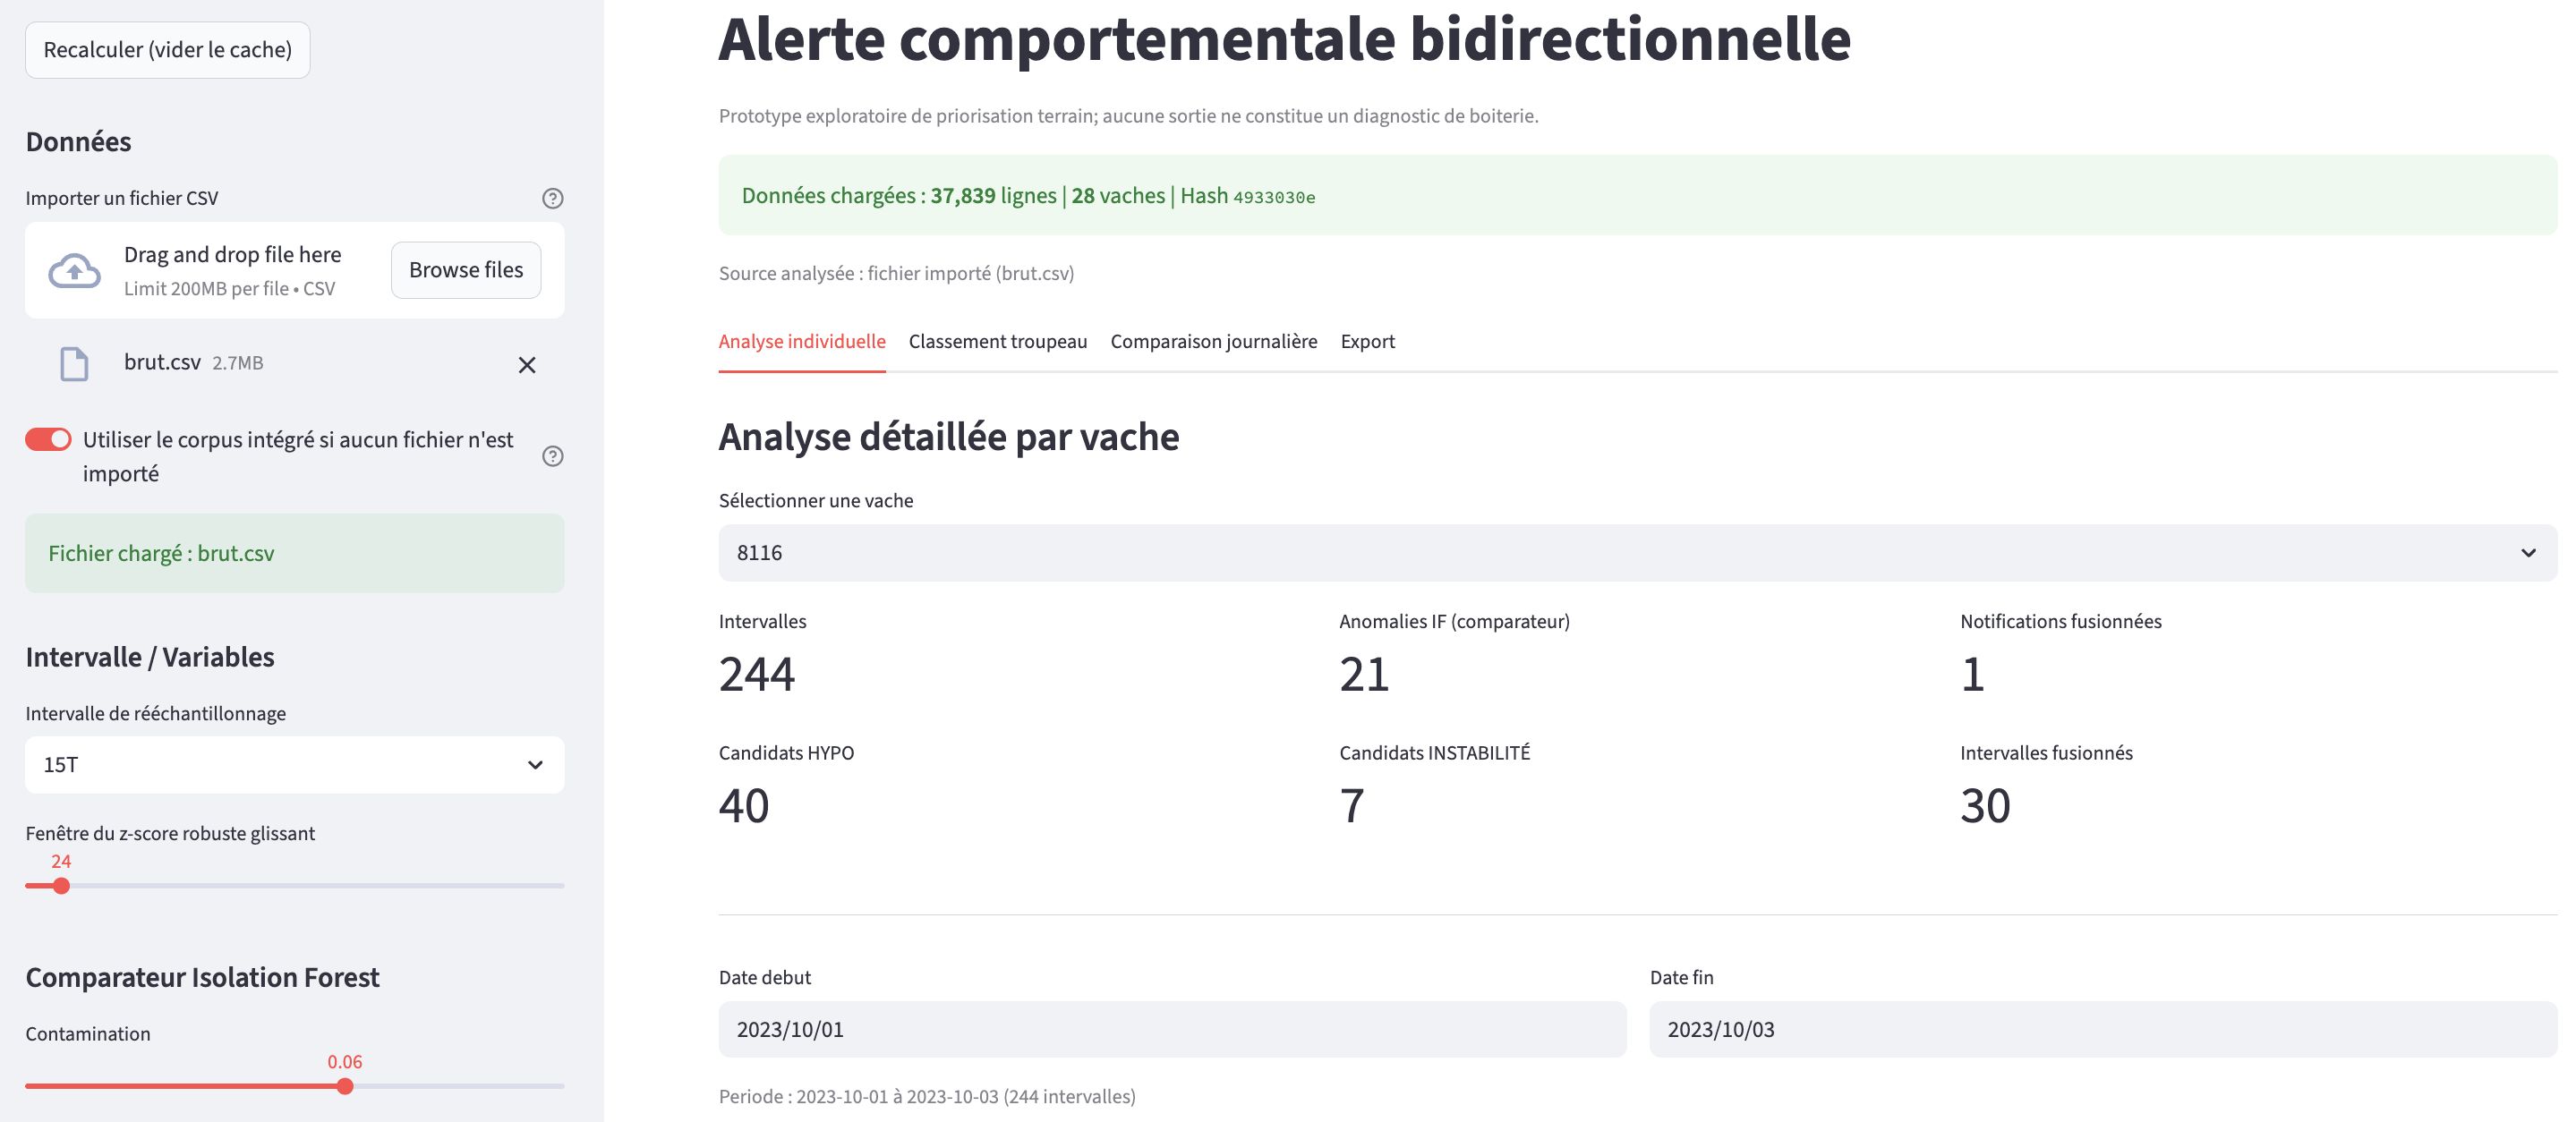
\includegraphics[width=0.98\textwidth]{figures/streamlit_overview.png}
  \caption{Vue d'ensemble du tableau de bord.}
  \label{fig:streamlit_overview}
\end{figure}

Les Figures~\ref{fig:streamlit_individual} à~\ref{fig:streamlit_heatmap} montrent comment une
même alerte est examinée à trois échelles complémentaires~: 1-~les signaux d'une vache,
2-~son rang dans le troupeau et 3-~la distribution journalière des alertes. Les marqueurs
localisent les intervalles à examiner, le classement et la carte thermique organisent l'ordre
de vérification.

Sur une fenêtre de trois jours, la vue individuelle superpose les variables retenues à
l'affichage~: l'indice de mouvement, les pas et le temps couché. Dans la
Figure~\ref{fig:streamlit_individual}, la légende nomme ces marqueurs~: \emph{Anomalie IF} en
bleu-vert, \emph{Épisode HYPO} en rouge, \emph{Épisode INSTABILITÉ} en ambre et
\emph{Notification} pour l'étoile violette qui ouvre l'épisode. Superposer ces marqueurs aux signaux bruts permet de
vérifier qu'une notification s'appuie sur une dégradation étendue dans le temps plutôt que
sur une valeur isolée. Les anomalies du comparateur restent affichées à titre de repère~;
elles ne déclenchent aucune notification.

% Page paysage, meme dispositif que la figure des vaches a verifier et que
% celle du chapitre 6 : trois panneaux superposes sur trois jours restent
% denses a la largeur du texte, la vue pivotee leur donne un tiers de largeur
% en plus. Le folio normal tomberait sur le bord gauche une fois la page
% pivotee, on le neutralise et on le replace, pivote, au bas de la vue.
\begin{landscape}
  \thispagestyle{empty}%
  \AddToShipoutPictureFG*{%
    \AtPageLowerLeft{\raisebox{0.5\paperheight}{\makebox[\paperwidth][r]{%
      \rotatebox{90}{\makebox[0pt][c]{\thepage}}\hspace{1.9cm}}}}%
  }%
  \vspace*{\fill}
  \begin{figure}[H]
    \centering
    % La capture fait 2582 px. Etalee sur 0,99 de la ligne en paysage, soit
    % 8,94 pouces, elle rend a 289 ppp, juste sous le seuil d'impression usuel
    % mais sans perte visible a cette taille de trait. Le paysage gagne en
    % echange un tiers de largeur.
    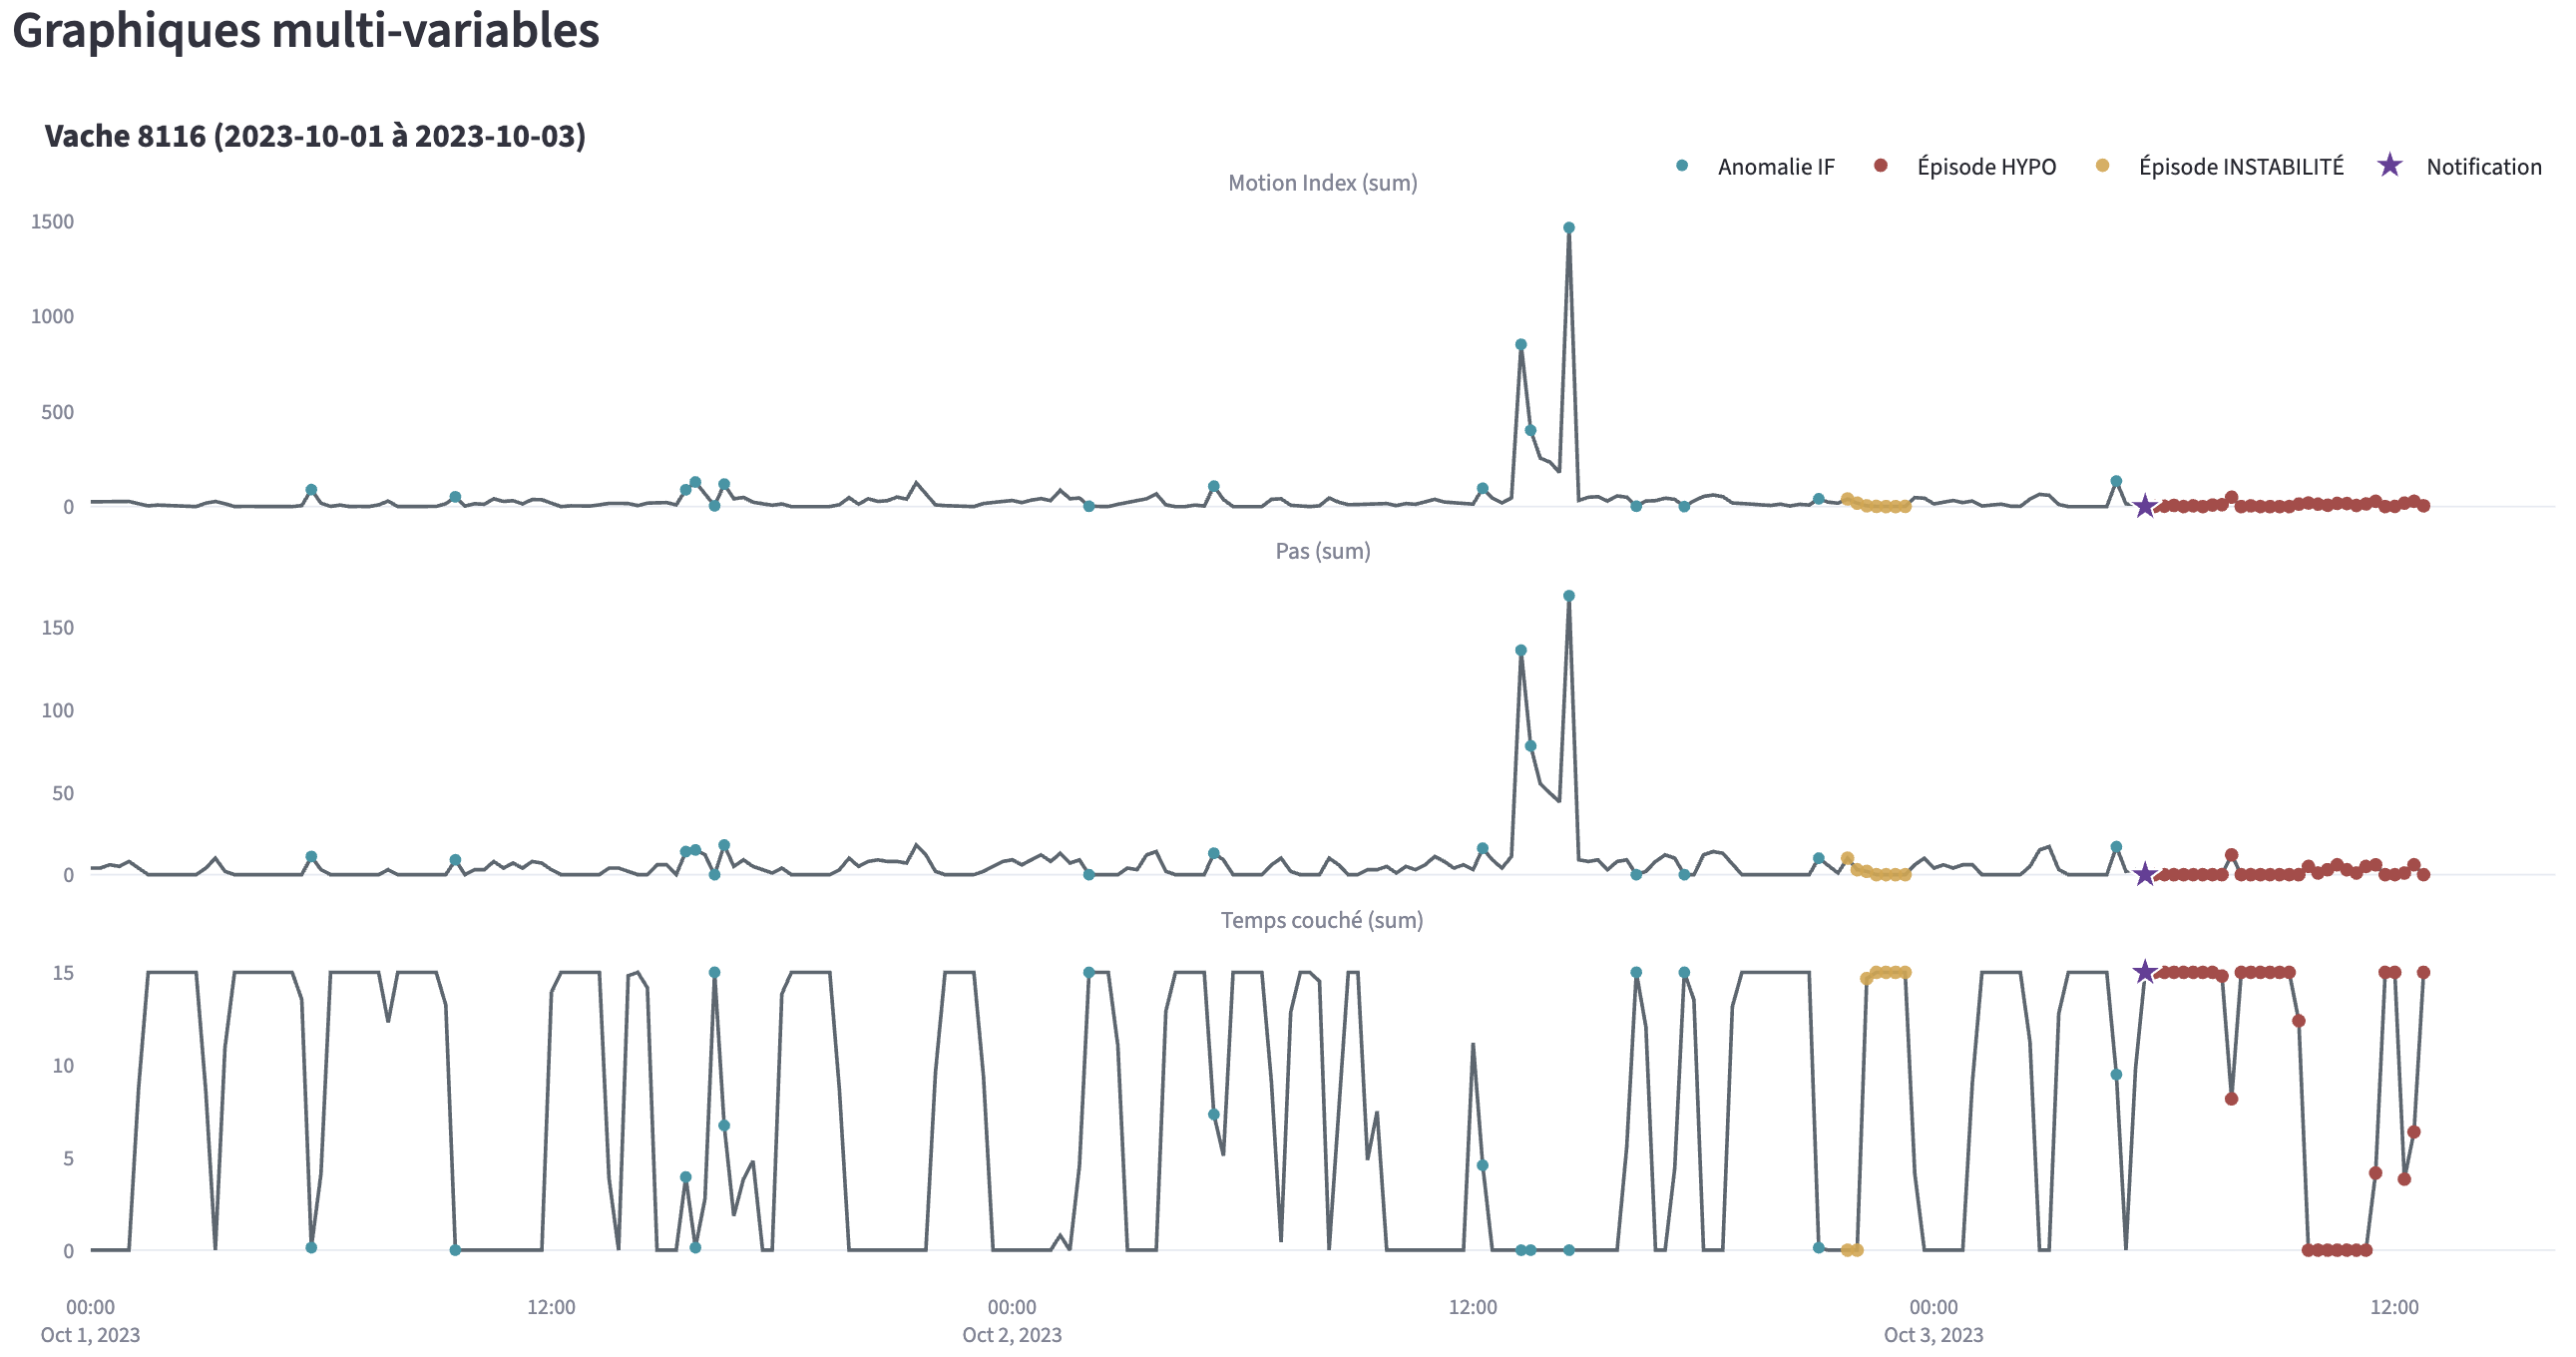
\includegraphics[width=0.99\linewidth]{figures/streamlit_individual.png}
    \caption{Analyse individuelle du tableau de bord.}
    \label{fig:streamlit_individual}
  \end{figure}
  \vfill
\end{landscape}

Le classement ordonne ensuite les vaches exploitables par priorité de vérification
(Figure~\ref{fig:streamlit_herd_table}). La colonne de rang donne l'ordre dans lequel les
aborder, tandis que les colonnes HYPO et INSTABILITÉ séparent les deux branches à l'origine
des notifications fusionnées~: un même rang peut provenir d'une hypoactivité persistante ou
d'une instabilité isolée, ce que le seul décompte fusionné ne dirait pas. Les colonnes de
couverture qualifient la fiabilité de la donnée sous-jacente~; un rang élevé associé à une
couverture faible appelle d'abord une vérification du capteur avant une observation de
la vache. La colonne d'anomalies Isolation Forest y figure au même titre que dans la vue
individuelle, comme comparateur.

\begin{figure}[H]
  \centering
  % La capture des vingt-huit rangs fait 1992 px de large : a 0,98 de la
  % largeur du texte, soit 6,40 pouces, elle rend a 311 ppp. La largeur maximale
  % est prise a dessein, ce tableau etant celui dont le corps se reduit le plus
  % une fois ramene a la page.
  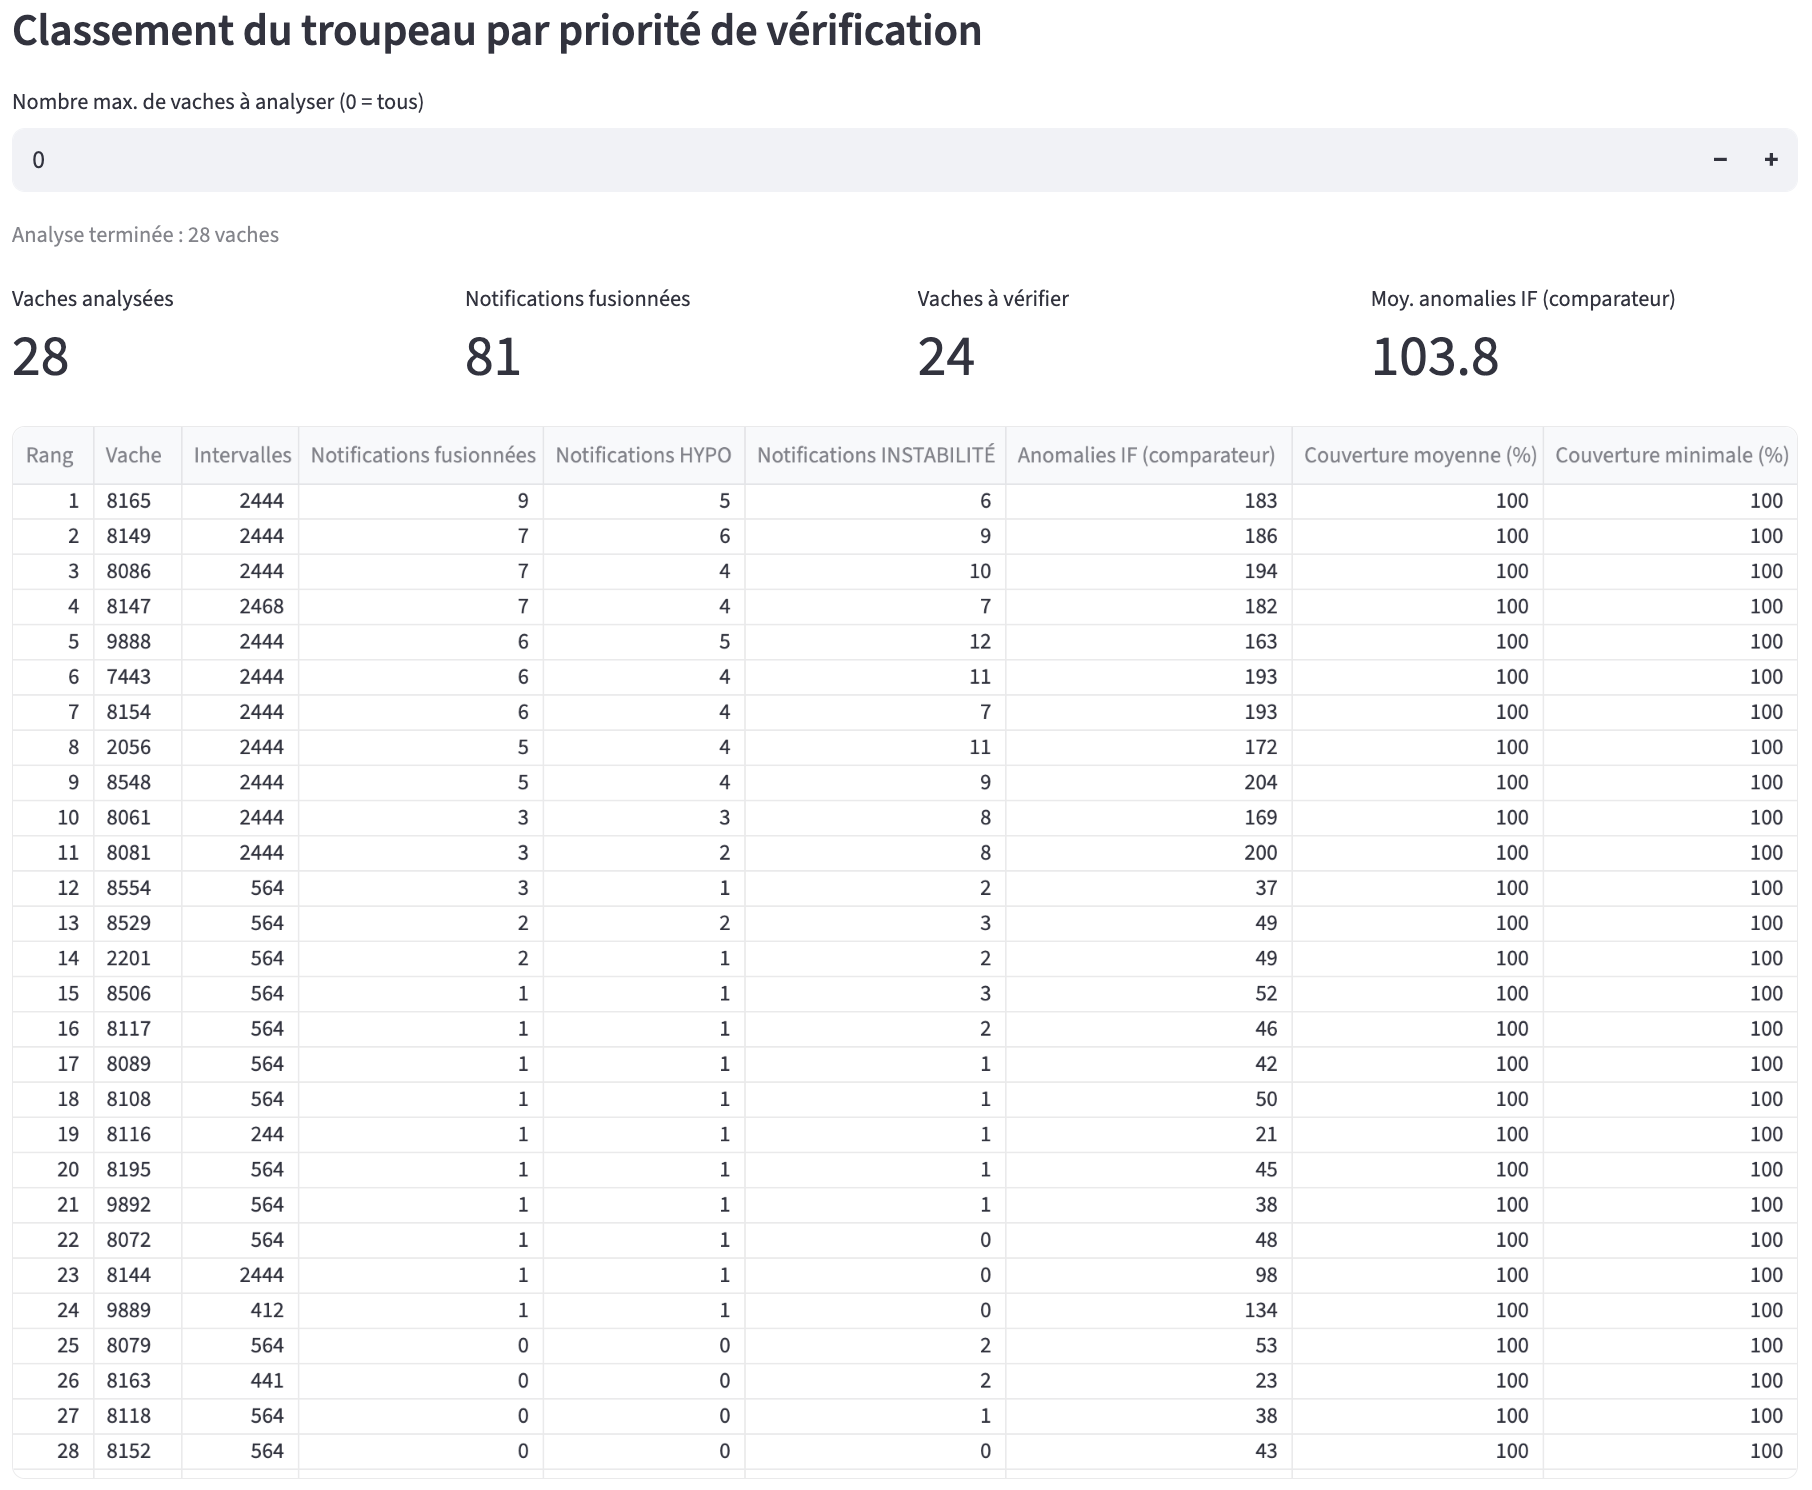
\includegraphics[width=0.98\textwidth]{figures/streamlit_herd_table.png}
  \caption{Onglet de classement du troupeau par priorité de vérification.}
  \label{fig:streamlit_herd_table}
\end{figure}

Chaque ligne de la Figure~\ref{fig:streamlit_heatmap} correspond enfin à une vache, chaque
colonne à une journée, et l'intensité traduit la sévérité des alertes de la journée. Cette
lecture déplace le regard de la vache vers le troupeau et fait apparaître des regroupements
qu'un classement cumulé masque~: une suite de journées consécutives sur une même vache ne se
lit pas comme quelques journées dispersées, et plusieurs vaches alertées le même jour
orientent vers une cause commune, de conduite ou de logement, plutôt que vers un problème
individuel. Les journées et les vaches sans mesure y restent grises, une absence de donnée
n'étant pas une absence d'alerte. La courbe placée dessous donne le nombre de vaches en alerte
et celui des vaches observées.

\begin{figure}[H]
  \centering
  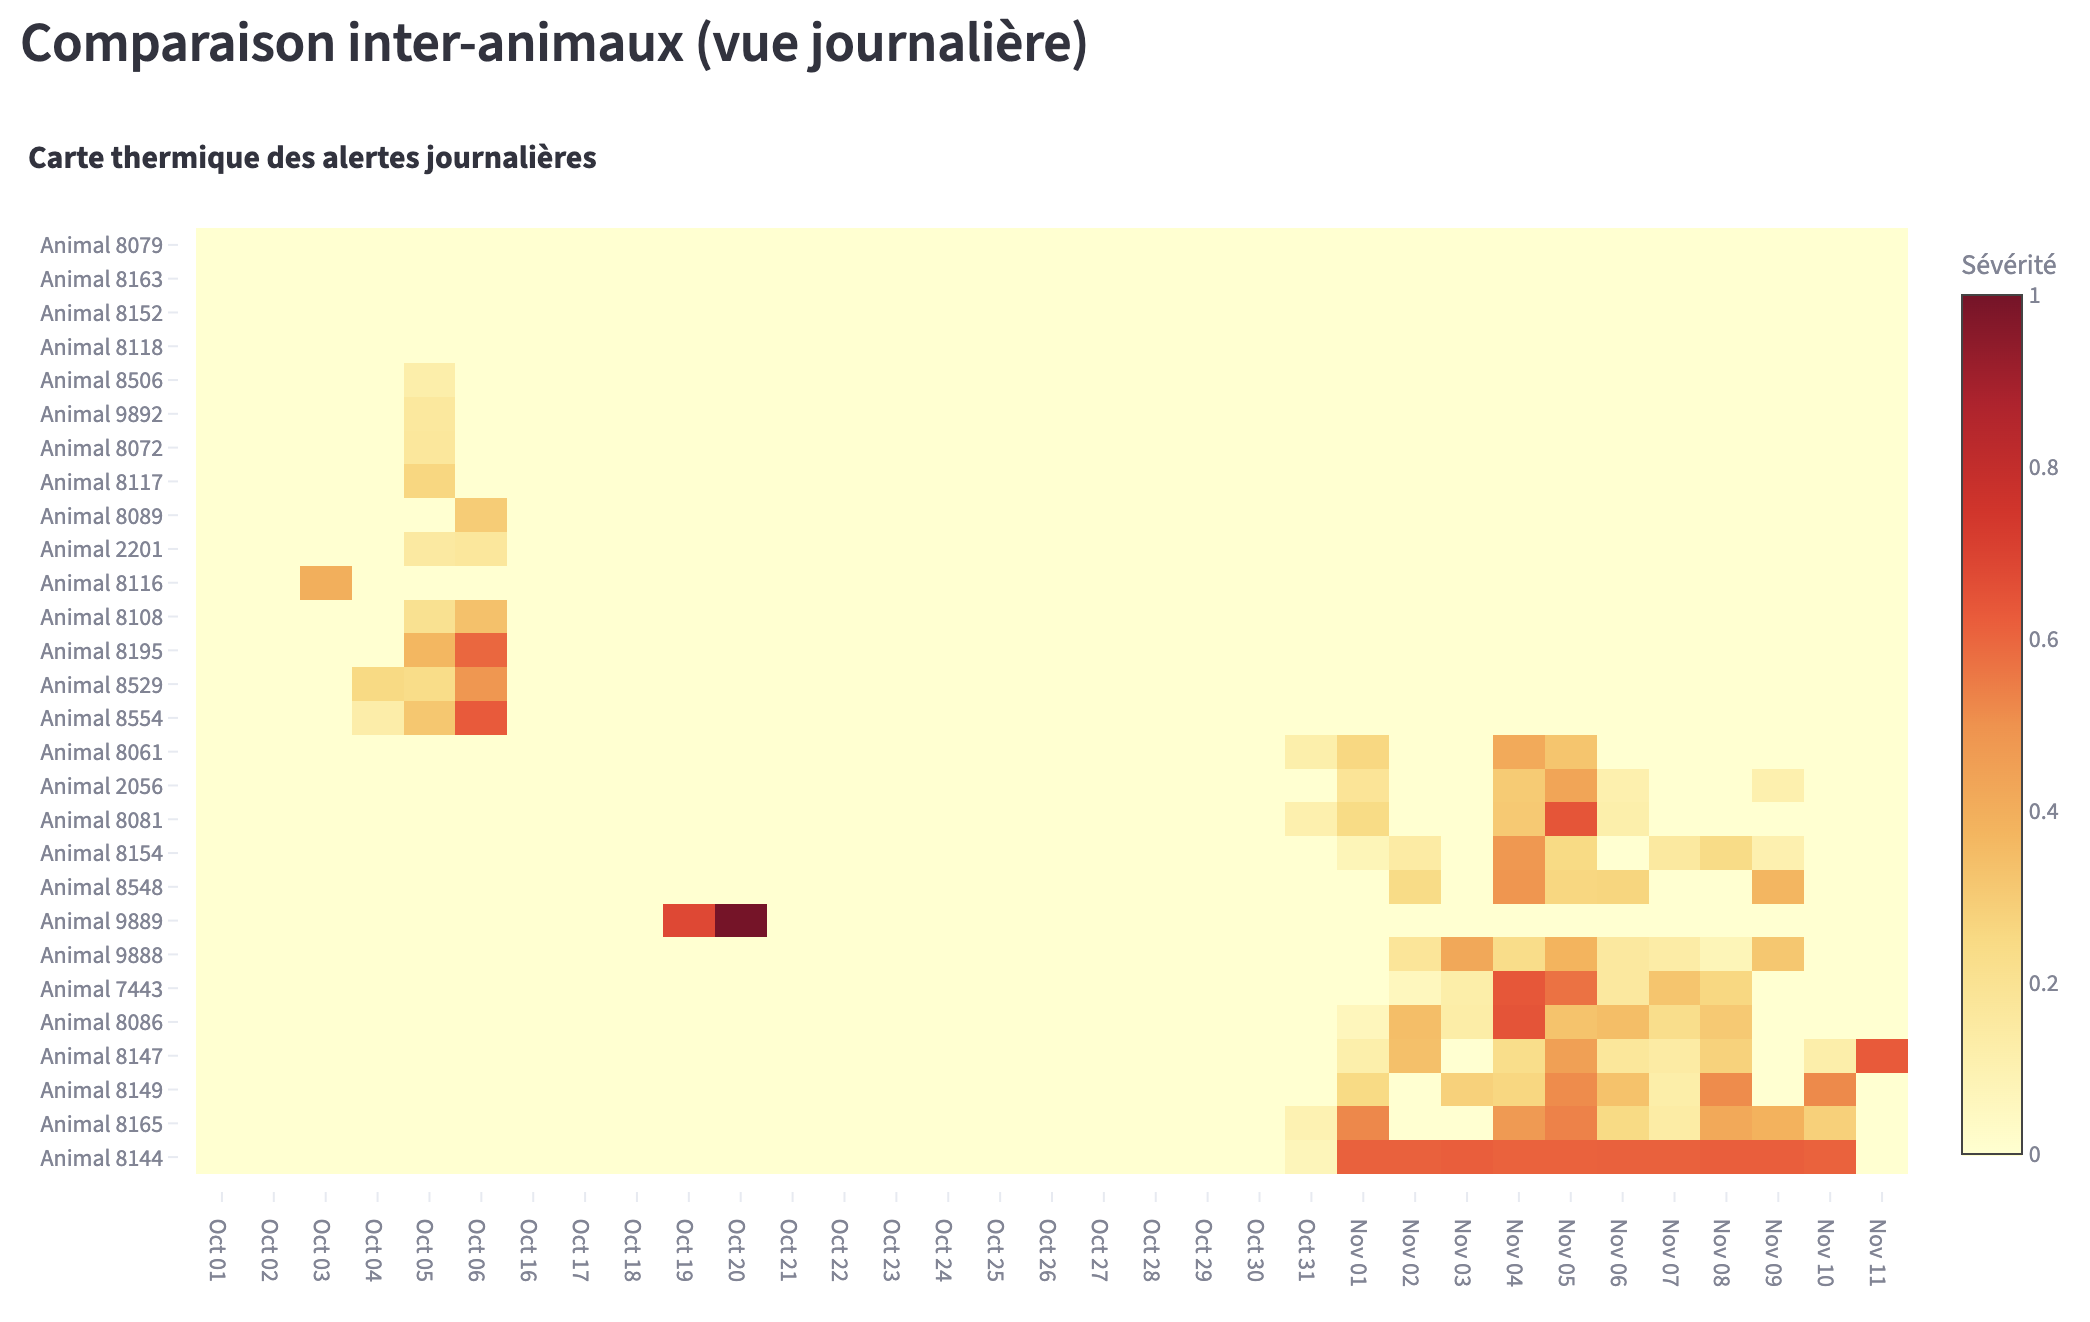
\includegraphics[width=0.98\textwidth]{figures/streamlit_heatmap_compact.png}
  \caption{Alertes journalières par vache et effectifs quotidiens du troupeau.}
  \label{fig:streamlit_heatmap}
\end{figure}

% =====================================================================
\section{Niveaux de priorité et action associée}
% =====================================================================
L'interface traduit la sortie de fusion en trois niveaux de priorité qui orientent l'effort
de vérification, comme le montre le Tableau~\ref{tab:priorites}. Seules les
priorités~2 et~3 produisent une notification de vérification~; la priorité~1 reste un signal de
surveillance.

Le choix de trois niveaux discrets, plutôt que d'un score continu, tient à la décision qu'ils
doivent servir. Sur le terrain, la question n'est pas de comparer des dixièmes entre deux
vaches, mais de trancher entre trois gestes~: se déplacer aujourd'hui, planifier une
observation, ou ne rien faire. Trois niveaux couvrent exactement ces trois issues. Un score
continu, lui, suggérerait une finesse de discrimination que les données n'autorisent pas~:
le corpus principal ne comporte aucun étalon vétérinaire qui permettrait de calibrer une
échelle, et afficher deux décimales reviendrait à donner du crédit à des écarts que rien ne
valide.

Ces niveaux reprennent directement la règle de fusion hiérarchique décrite au
Chapitre~\ref{chapitre:systeme}, sans la réinterpréter. La priorité~3 correspond aux
situations où les deux branches concordent, par convergence simultanée ou par séquence~: le
comportement s'y écarte de plusieurs manières à la fois, ce qui rend l'écart plus difficile à
attribuer au hasard ou à un artefact de mesure. La priorité~2 correspond à une hypoactivité
persistante seule, la branche dont le Chapitre~\ref{chapitre:resultats} montre qu'elle est la
mieux étayée. La priorité~1 correspond à une instabilité isolée, tenue à distance de la
notification tant qu'aucune baisse d'activité ne l'accompagne.

\begin{table}[H]
  \centering
  \caption{Niveaux de priorité de l'interface et action de vérification associée.}
  \label{tab:priorites}
  \small
  \begin{tabular}{cp{0.36\textwidth}p{0.38\textwidth}}
    \toprule
    Priorité & Condition & Action suggérée \\
    \midrule
    3 & Convergence HYPO + INSTABILITÉ, ou séquence instabilité$\rightarrow$hypoactivité &
    Vérification rapprochée, observation locomotrice \\
    2 & Hypoactivité persistante (HYPO) & Vérification à planifier \\
    1 & Instabilité isolée & Surveillance, sans alerte de vérification \\
    \bottomrule
  \end{tabular}
\end{table}

Cette gradation traduit une asymétrie de coût plutôt qu'une échelle de gravité. Un déplacement
inutile coûte quelques minutes~; une dégradation ignorée coûte du temps d'évolution, et c'est
précisément ce temps que la détection précoce cherche à récupérer. Les priorités~2 et~3
déclenchent donc une notification, quitte à ce qu'une part d'entre elles ne débouche sur rien.
La priorité~1, à l'inverse, se contente d'attirer l'attention~: elle signale une situation à
regarder si l'occasion se présente, sans imposer de geste ni entrer dans le décompte des
vérifications à effectuer. Séparer ces deux régimes évite qu'une piste exploratoire, dont le
lien avec la boiterie reste à établir, ne se transforme en charge de travail quotidienne.

Une même situation ne remonte pas indéfiniment~: une période réfractaire suit chaque
notification, de sorte qu'un épisode qui se prolonge apparaît une fois plutôt que d'occuper la
liste à chaque intervalle. Ce mécanisme, décrit au Chapitre~\ref{chapitre:systeme}, importe
autant que le seuil lui-même~: sans lui, une seule vache en dégradation lente saturerait le
classement et masquerait les autres.

À l'écran, chaque vache retenue est accompagnée du décompte de ses notifications fusionnées,
HYPO et INSTABILITÉ, et d'une vignette qui situe ses épisodes dans la période observée, comme
le représente la Figure~\ref{fig:streamlit_priority_animals}. L'ordre de vérification et le
motif qui le justifie se lisent ainsi ensemble, sans qu'il soit nécessaire de revenir à la
vue individuelle de chaque vache.

% Page paysage. Six vignettes sur deux colonnes restent illisibles a la largeur
% du texte : la vue pivotee leur donne un quart de largeur en plus, et c'est la
% lisibilite qui prime ici sur la finesse d'impression. Meme
% dispositif qu'au chapitre 6 : le folio normal tomberait sur le bord gauche
% une fois la page pivotee, on le neutralise et on le replace, pivote, au bas
% de la vue.
\begin{landscape}
  \thispagestyle{empty}%
  \AddToShipoutPictureFG*{%
    \AtPageLowerLeft{\raisebox{0.5\paperheight}{\makebox[\paperwidth][r]{%
      \rotatebox{90}{\makebox[0pt][c]{\thepage}}\hspace{1.9cm}}}}%
  }%
  % Ressorts elastiques de part et d'autre : la figure se cale au milieu de la
  % hauteur de page au lieu de rester en haut, le blanc se repartissant alors
  % egalement au-dessus et au-dessous.
  \vspace*{\fill}
  \begin{figure}[H]
    \centering
    % 0,96 et non 0,98 : la capture fait 2526 px pour un rapport de 1,56, si bien
    % qu'a 0,98 la figure et sa legende depasseraient la hauteur disponible. Un
    % depassement de trois dixiemes de point suffit ici a repousser le flottant
    % et a ajouter une page. A 0,96 elle occupe 5,55 pouces sur 8,67 de large et
    % rend a 291 ppp, juste sous le seuil usuel mais sans perte visible sur un
    % trace au trait. La largeur reste prise au plus haut : les graduations et
    % les dates des vignettes ne se lisent qu'a cette taille.
    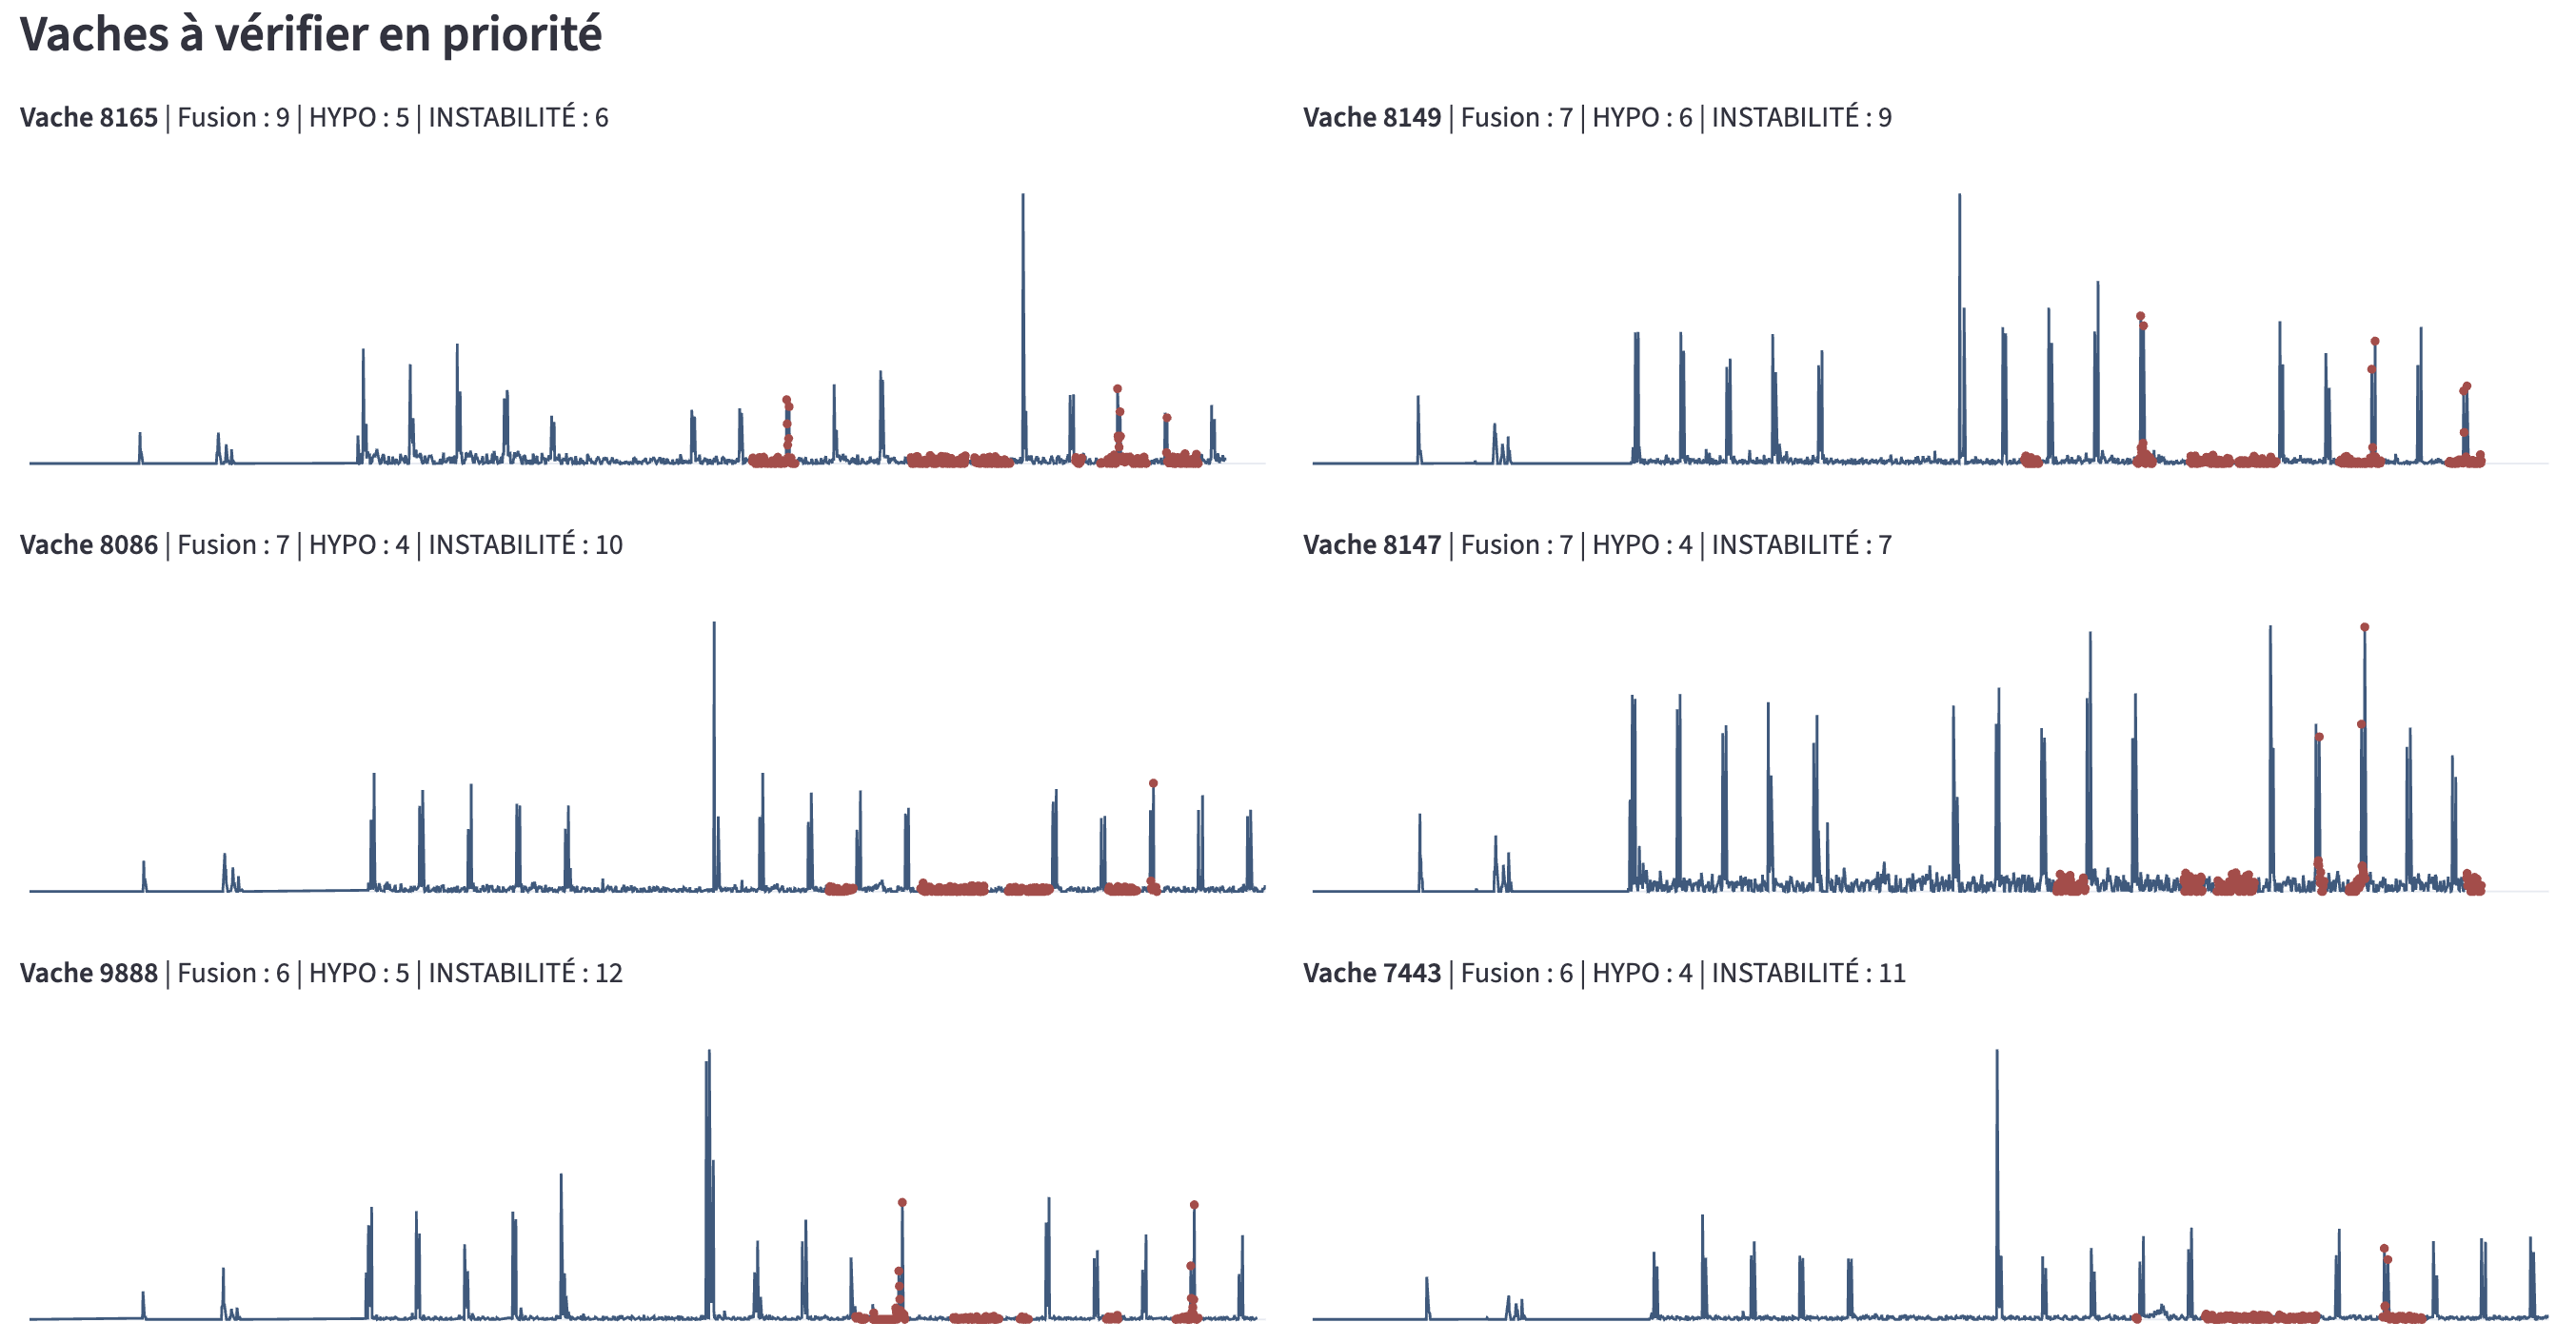
\includegraphics[width=0.96\linewidth]{figures/streamlit_priority_animals.png}
    \caption{Vaches à vérifier en priorité.}
    \label{fig:streamlit_priority_animals}
  \end{figure}
  \vfill
\end{landscape}

% =====================================================================
\section{Export et traçabilité des alertes}
% =====================================================================
Une priorité affichée n'a d'utilité que si elle peut sortir de l'écran. L'interface expose
donc un onglet d'export qui produit trois fichiers CSV~: un résumé par vache, les données
complètes du troupeau au grain de l'intervalle, et les alertes comportementales,
c'est-à-dire les débuts d'épisode retenus par la fusion. La vue individuelle permet en outre
d'exporter la série d'une vache telle qu'elle est affichée, avec les filtres appliqués. Ces fichiers
alimentent le registre d'élevage ou une vérification hors ligne, sans imposer que l'interface
reste ouverte.

La table individuelle et son export correspondent à la chaîne actuelle: épisodes et
notifications de la fusion, candidats HYPO, surveillance d'instabilité, couverture et
partition chronologique. Les sorties d'Isolation Forest y sont conservées uniquement comme
comparateur explicitement nommé. Les anciennes colonnes cliniques de la première chaîne ne
sont ni affichées ni exportées, afin qu'un résultat historique ne puisse être confondu avec
une sortie du système évalué dans ce mémoire. Le fichier CSV individuel contient exactement
les lignes visibles après application des filtres.

La traçabilité repose sur le nommage. Chaque fichier exporté porte la résolution temporelle
retenue et une empreinte courte du fichier source, calculée au chargement et affichée à
l'écran. L'export individuel y ajoute l'identifiant de la vache et la fenêtre de dates. Deux
exports issus de jeux de données ou de résolutions différents ne peuvent donc pas être
confondus, et un fichier retrouvé plusieurs semaines plus tard reste rattachable à son
origine. Cette empreinte sert à identifier une source, non à garantir son intégrité
cryptographique~: cette garantie relève du manifeste SHA-256 de la chaîne reproductible
(Annexe~\ref{annexe:validation}), dont ce nommage prolonge la logique à l'échelle de
l'interface.

% =====================================================================
\section{Portée et limites de l'usage en ferme}
% =====================================================================
L'interface est un prototype de démonstration. Elle s'exécute localement, charge un fichier
CSV et montre que les sorties du détecteur peuvent être lues, ordonnées et rattachées à des
vaches précises. Elle n'est pas un produit déployé~: elle ne gère ni l'acquisition continue
des mesures, ni les comptes utilisateurs, ni l'historique des vérifications réalisées.

L'usage prévu de l'interface est donc étroit, et cette étroitesse est assumée. Une priorité~3 signifie que
la vache mérite d'être regardée avant les autres, non qu'elle est boiteuse. Aucune vue
n'autorise à conclure à une boiterie sans examen du pied.

Une limite tient à l'évaluation de l'outil lui-même~: l'interface n'a pas été soumise à des
utilisateurs. Aucun éleveur ni technicien n'a été observé en train de s'en servir, et la
lisibilité des vues, le temps nécessaire pour trancher un cas et l'acceptabilité des
trois niveaux de priorité n'ont pas été mesurés. Les choix de présentation découlent du
positionnement du mémoire et des contraintes du détecteur, non d'une étude d'usage. Une
évaluation auprès d'utilisateurs réels constitue donc une étape nécessaire avant tout
déploiement, au même titre que la validation clinique du détecteur. La charge de vérification
que ce classement par priorité représente et ses conséquences pratiques pour l'éleveur sont examinées dans la
discussion générale.

\chapter{Résultats et analyses}
\label{chapitre:resultats}

Ce chapitre présente les preuves techniques du système. La première partie montre la réponse
de la branche HYPO à des dégradations graduelles, son
avantage sur les comparateurs IF/LOF et sa stabilité locale par OFAT. La deuxième partie
teste sa robustesse à des formes moins favorables à aire d'enveloppe appariée, puis examine l'extension
INSTABILITÉ et les règles de fusion sur une campagne plus large. Les
pourcentages décrivent la réponse du logiciel à des scénarios contrôlés et permettent de
comparer la détection, la localisation et la charge de vérification. Le Tableau~\ref{tab:cles_lecture_resultats}
présente les clés de lecture mobilisées tout au long de ce chapitre.

Aucun étalon vétérinaire n'accompagne le corpus principal~: la performance ne se lit donc pas
en valeur absolue. Elle se juge de trois façons. La première est l'écart à l'exécution propre
de la même vache, qui isole ce que l'injection seule produit. La deuxième est la comparaison
aux quatre configurations alternatives appliquées aux mêmes fenêtres, qui situe l'apport de la
structure temporelle et multivariée. La troisième est le respect des conditions de portée
fixées au Chapitre~\ref{chapitre:systeme} avant la campagne, pour la sélection des règles de
fusion. Le Tableau~\ref{tab:objectifs_resultats}, en fin de chapitre, confronte chaque
objectif annoncé à son résultat.

% =====================================================================
\section{Clés de lecture et intégrité des protocoles}
% =====================================================================
\begin{table}[H]
  \centering
  \caption{Clés de lecture du chapitre.}
  \label{tab:cles_lecture_resultats}
  \small
  \begin{tabular}{p{0.28\textwidth}p{0.64\textwidth}}
    \toprule
    Élément & Interprétation \\
    \midrule
    Vaches admissibles
      & Seules onze des 28 vaches possèdent une période future suffisamment longue, les signaux
        requis et une couverture compatible avec toutes les campagnes. \\
    Injections après la période de référence
      & Elles commencent après les 60\,\% réservés à la construction de la référence; les
        données injectées ne peuvent donc pas influencer cette référence. \\
    Attribution
      & Une alerte est attribuable seulement si elle apparaît avec l'injection et non dans
        l'exécution propre de la même vache et de la même période. \\
    Couverture
      & Au moins un intervalle attribuable recouvre la fenêtre injectée. \\
    Nouveau départ
      & Un épisode absent de l'exécution propre commence dans la fenêtre; ce critère est plus
        exigeant qu'un simple recouvrement. \\
    IoU20
      & Le recouvrement temporel entre l'épisode attribuable et l'événement atteint au moins
        0,20; il renseigne la localisation temporelle de l'épisode. \\
    Charge de fond
      & Les notifications hors fenêtres injectées sur des données non étiquetées; elles
        mesurent l'effort de vérification attendu. \\
    Hypoactivité non locomotrice
      & Neuf alertes sur onze montrent que les signaux disponibles ne permettent pas
        d'identifier la cause d'une baisse persistante. \\
    \bottomrule
  \end{tabular}
\end{table}

Les onze vaches admissibles fournissent quatre événements par vache lors de la campagne
HYPO, soit un total de 44 événements, six formes à trois positions dans le stress test, pour
un total de 198 événements, ainsi que douze scénarios par vache lors de la campagne étendue,
pour un total de 132 scénarios. Ces effectifs ne sont
pas regroupés~: la première campagne mesure la réponse attribuable de HYPO, la deuxième
éprouve la forme temporelle sans changer la dose, tandis que la troisième examine
INSTABILITÉ et les règles de fusion sur un éventail plus large de situations. Le
Tableau~\ref{tab:protocol_checks} récapitule les contrôles automatiques qui garantissent
l'intégrité et la comparabilité de ces campagnes.

\begin{table}[H]
  \centering
  \caption{Contrôles automatiques communs aux campagnes techniques.}
  \label{tab:protocol_checks}
  \begin{tabular}{p{0.68\textwidth}c}
    \toprule
    Contrôle & Résultat \\
    \midrule
    Colonnes requises présentes et campagnes non vides & Conforme \\
    Identifiants et fenêtres physiques uniques & Conforme \\
    Fenêtres non chevauchantes dans la campagne HYPO & Conforme \\
    Injections strictement postérieures à la période de référence & Conforme \\
    Signaux sources informatifs et couverture admissible & Conforme \\
    Non-négativité et conservation du temps postural & Conforme \\
    Aire d'enveloppe appariée sur les intervalles conservés du stress test & Conforme \\
    Trois positions postérieures à la période de référence & Conforme \\
    Exécution propre utilisée pour l'attribution & Conforme \\
    \bottomrule
  \end{tabular}
\end{table}

Les neuf contrôles sont conformes sur les trois campagnes. Ils vérifient la structure des
fichiers, l'unicité des identifiants et des fenêtres, la postériorité des injections par
rapport à la période de référence, l'appariement de l'aire d'enveloppe et la conservation du
temps postural. Un seul contrôle en échec invaliderait la campagne concernée, car tous les
résultats rapportés ensuite supposent ces conditions réunies.

% =====================================================================
\section{Performance attribuable du module HYPO}
% =====================================================================
\subsection{Résultats attribuables par profil}
Le Tableau~\ref{tab:hypo_profiles} présente les résultats attribuables par profil. Il
s'agit du nouveau départ, de la couverture attribuable et de la localisation IoU20. Les trois
profils graduels, léger, modéré et marqué, sont les cas techniques attendus positifs, alors
que la variation brève isolée représente le contrôle attendu négatif. Les valeurs agrégées
rapportées plus bas portent sur les 33 dégradations graduelles, c'est-à-dire sur ces trois
profils réunis.

\begin{table}[H]
  \centering
  \caption{Résultats attribuables du module HYPO.}
  \label{tab:hypo_profiles}
  \small
  \begin{tabular}{lrrrrr}
    \toprule
    Profil & $n$ & Nouveau départ & Couverture & IoU20 & IoU moyen \\
    \midrule
    Graduel léger & 11 & 45,5\,\% & 72,7\,\% & 27,3\,\% & 0,087 \\
    Graduel modéré & 11 & 63,6\,\% & 90,9\,\% & 36,4\,\% & 0,192 \\
    Graduel marqué & 11 & 63,6\,\% & 100,0\,\% & 54,5\,\% & 0,269 \\
    Variation brève isolée & 11 & 0,0\,\% & 0,0\,\% & 0,0\,\% & 0,000 \\
    \bottomrule
  \end{tabular}
\end{table}

Comme le montre le Tableau~\ref{tab:hypo_profiles}, un nouvel épisode apparaît dans 19 cas
sur les 33 dégradations graduelles, soit 57,6\,\%.
Après la soustraction de l'exécution propre, un intervalle ajouté recouvre la fenêtre dans
29 cas sur 33, soit 87,9\,\%, et 13 cas atteignent IoU~$\geq0{,}20$, soit 39,4\,\%.
L'IoU attribuable moyen est de 0,183 et le délai médian de nouveau départ de 20,75 heures.
Les intervalles de confiance à 95\,\%, obtenus par bootstrap regroupé par vache
\citep{efron1993introduction,fieldwelsh2007bootstrapping}
(10\,000~rééchantillonnages, l'unité étant la vache), sont [78,8~; 97,0] pour la couverture,
[42,4~; 75,8] pour le nouveau départ et [24,2~; 54,5] pour l'IoU20. Leur largeur reflète
l'effectif de onze vaches et invite à interpréter la valeur ponctuelle avec prudence.
Ces indicateurs ne sont pas interchangeables: la couverture montre une réponse dans la
fenêtre, tandis que le nouveau départ vérifie qu'un épisode distinct a réellement commencé.

Le contrôle bref n'engendre aucun départ ou intervalle attribuable. Sur les exécutions
propres et uniquement pendant la période future, HYPO produit en moyenne 0,402
notification par vache-jour; le 90\textsuperscript{e} percentile entre vaches est de 0,491.
Cette quantité mesure l'effort de vérification attendu sur la période surveillée; elle est
rapportée séparément des métriques attribuables pour éviter de confondre charge opérationnelle
et détection des événements injectés.

\subsection{Typologie des modes de défaillance}
Le Tableau~\ref{tab:failure_modes} décompose les résultats actuels en modes d'échec, sans
reprendre les fréquences d'un protocole antérieur. Sur les 33 dégradations graduelles, 4
ne produisent aucun recouvrement attribuable et 16 sont recouvertes sans localisation
suffisante~; sur les 29 recouvertes, 10 n'ouvrent aucun nouveau départ par rapport à
l'exécution propre. Du côté des contrôles, les variations brèves sont rejetées, mais
l'hypoactivité non locomotrice déclenche 9 alertes sur 11. Parmi les 33 instabilités
pures, 22 sont repérées par la branche de surveillance et aucune ne produit un épisode
nécessitant une vérification de la fusion. Ces fréquences sont régénérées par le script
\path{scripts/compute_failure_modes.py}.

\begin{table}[H]
  \centering
  \caption{Modes de défaillance observés.}
  \label{tab:failure_modes}
  \small
  \begin{tabular}{p{0.62\textwidth}r}
    \toprule
    Mode & Fréquence \\
    \midrule
    Graduel non détecté (aucun recouvrement attribuable) & 4 / 33 \\
    Graduel recouvert mais mal localisé (IoU $<$ 0,20) & 16 / 33 \\
    Graduel recouvert sans nouveau départ & 10 / 29 \\
    Confusion avec une hypoactivité non locomotrice & 9 / 11 \\
    Instabilité pure repérée en surveillance & 22 / 33 \\
    Instabilité pure produisant un épisode de vérification & 0 / 33 \\
    Contrôle bref alerté à tort & 0 / 11 \\
    \bottomrule
  \end{tabular}
\end{table}

Cette typologie oriente les priorités~: la localisation temporelle et la séparation causale
avec les hypoactivités non locomotrices sont les deux limites dominantes, tandis que les pics
brefs sont rejetés dans les conditions testées.

\subsection{Compromis entre réponse technique et charge de fond}
Le seuil de score HYPO est ensuite parcouru de 0,04 à 0,20 sans modifier les autres paramètres.
Les 9 configurations rejettent les 11 variations brèves. Entre 0,04 et 0,12, la
couverture, les nouveaux départs et IoU20 conservent les valeurs de la configuration de
référence, soit 87,9\,\%, 57,6\,\% et
39,4\,\%, tandis que le fond diminue légèrement de 0,419 à 0,402 notification par
vache-jour. À 0,20, le fond atteint 0,330, mais la couverture et IoU20 baissent à 78,8\,\%
et 30,3\,\%.

Le point 0,14 atteint 45,5\,\% à IoU20 avec un fond de 0,375 et les mêmes taux de couverture
et de nouveaux départs que la référence. Il ne constitue toutefois pas un nouvel optimum~:
il a été observé sur le même ensemble qui sert à évaluer la configuration. Le seuil de 0,12
reste donc inchangé; 0,14 devient seulement une hypothèse à tester après sélection sur un
jeu de développement indépendant.

Dans la Figure~\ref{fig:detection_background_curve}, le panneau~(a) rapporte la réponse aux
injections et le panneau~(b) la charge de fond, les deux partageant le même axe des seuils.
La ligne pointillée y repère le seuil de
référence de 0,12, conservé malgré le résultat ponctuel observé à 0,14.

\begin{figure}[H]
  \centering
  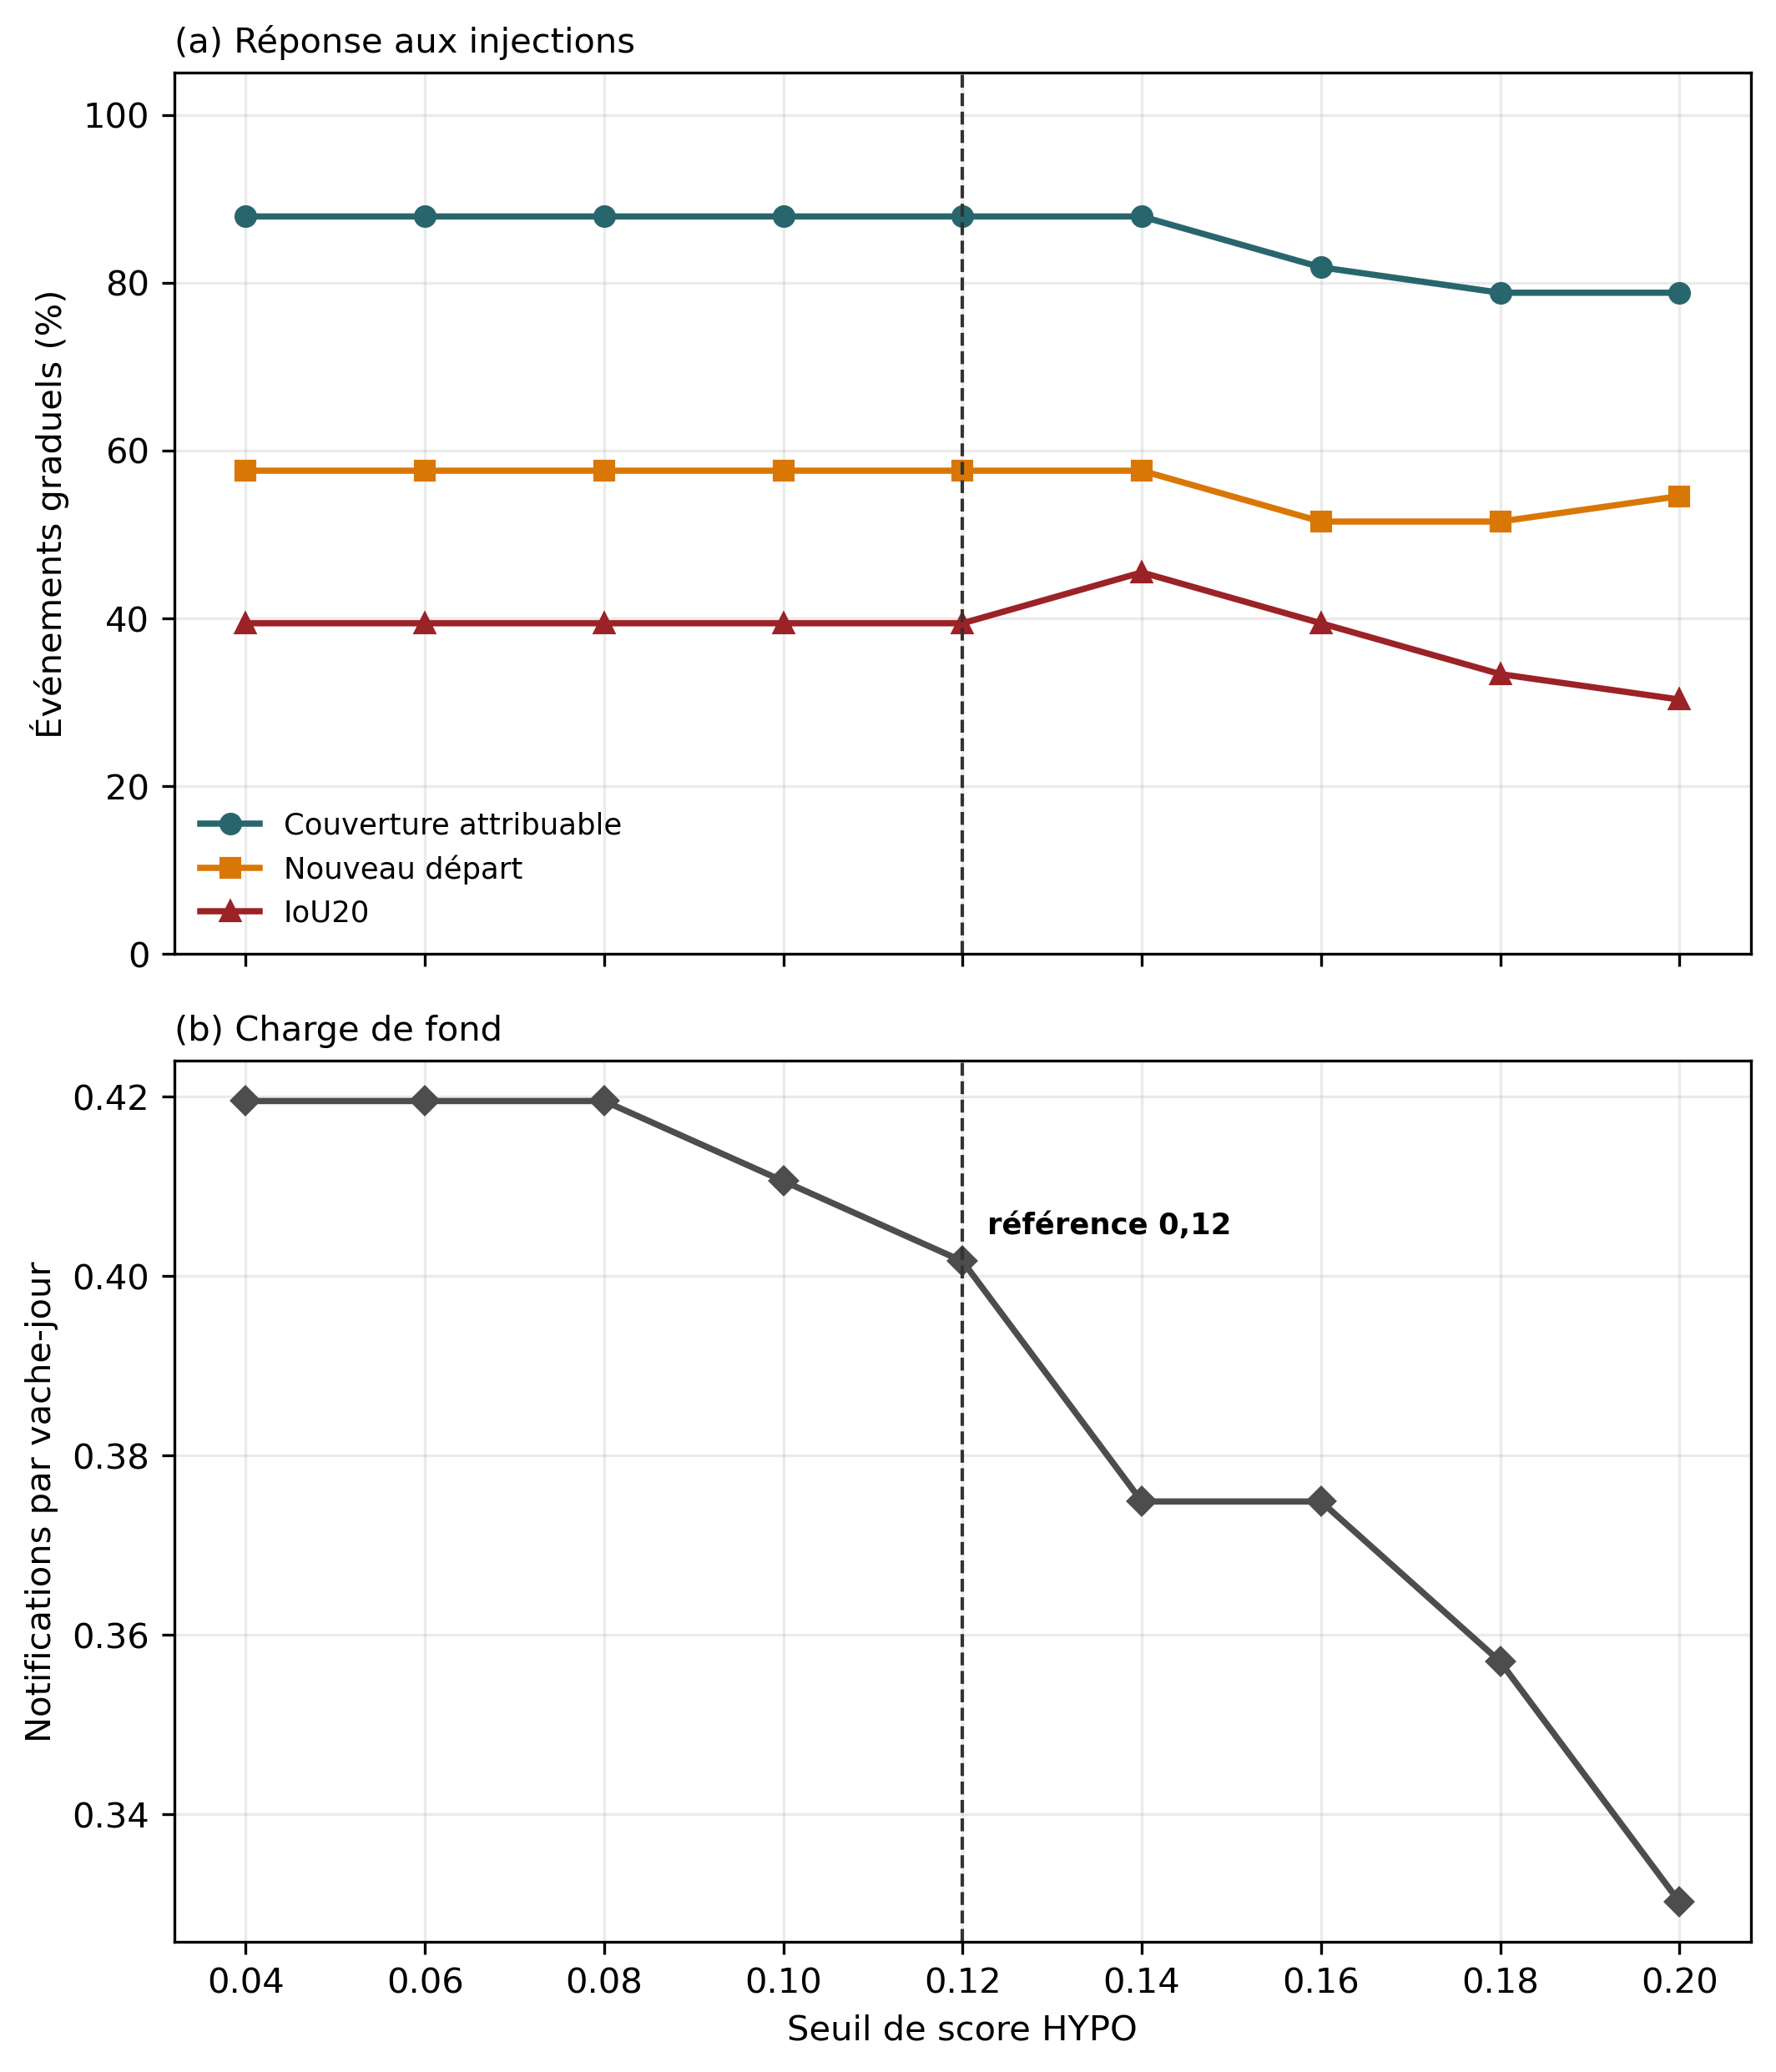
\includegraphics[width=0.98\textwidth]{figures/detection_background_curve.png}
  \caption{Compromis détection-charge de fond.}
  \label{fig:detection_background_curve}
\end{figure}

\subsection{Inspection visuelle ciblée}
La Figure~\ref{fig:manual_review} montre quatre situations de la vache 8081 après le gel
des paramètres. L'hypoactivité modérée produit un épisode de vérification, alors que
l'instabilité modérée reste au niveau de surveillance. Le pic capteur isolé est rejeté et
l'hypoactivité non
locomotrice produit une alerte comparable à celle d'une baisse locomotrice. Dans le premier
panneau, l'épisode est déjà actif à l'ouverture de la fenêtre~: il compte donc comme couverture
attribuable mais non comme nouveau départ, le critère exigeant un début absent de l'exécution
propre. La fenêtre injectée
apparaît en fond gris derrière les courbes, tandis que les sorties du système occupent un
bandeau distinct sous l'axe des signaux~: rouge pour un épisode de vérification, ambre pour une
période de surveillance sans alerte. Le rejet est ainsi la seule issue qui ne reçoit aucune
marque. Séparer la vérité injectée des sorties sur deux canaux distincts évite toute teinte
intermédiaire et rend leur recouvrement directement lisible. Chaque panneau affiche 12
heures de part et d'autre de la fenêtre injectée, et le bandeau rend compte de l'état du
système sur toute la période représentée, marges comprises~; l'issue annoncée dans le titre
porte en revanche sur la seule fenêtre injectée. Une bande de surveillance située hors de
cette fenêtre n'entre pas dans les taux rapportés, qu'elle relève du bruit de fond ou d'une
réaction différée à l'événement injecté comme au panneau du pic capteur, ce qui
explique qu'un panneau puisse en présenter alors que le scénario correspondant affiche un
taux de surveillance nul. Les traits verticaux pointillés
marquent les bornes exactes de la fenêtre injectée, y compris lorsqu'elle ne dure qu'un seul
pas de temps. Dans chaque panneau, les trois
signaux sont tracés bruts en transparence sous une moyenne glissante horaire, et normalisés
séparément par le maximum de cette moyenne : un pic isolé ne comprime donc plus le reste de la
courbe contre l'axe. Cette inspection vérifie la cohérence technique des sorties.

% Page paysage. Le folio normal tomberait sur le bord gauche une fois la page
% pivotee : on le neutralise et on le replace, pivote, au bas de la vue paysage
% pour qu'il se lise comme sur toutes les autres pages. Le flottant est fixe par
% [H] afin que la figure ne se deplace pas d'une compilation a l'autre.
\begin{landscape}
  \thispagestyle{empty}%
  \AddToShipoutPictureFG*{%
    \AtPageLowerLeft{\raisebox{0.5\paperheight}{\makebox[\paperwidth][r]{%
      \rotatebox{90}{\makebox[0pt][c]{\thepage}}\hspace{1.9cm}}}}%
  }%
  \begin{figure}[H]
    \centering
    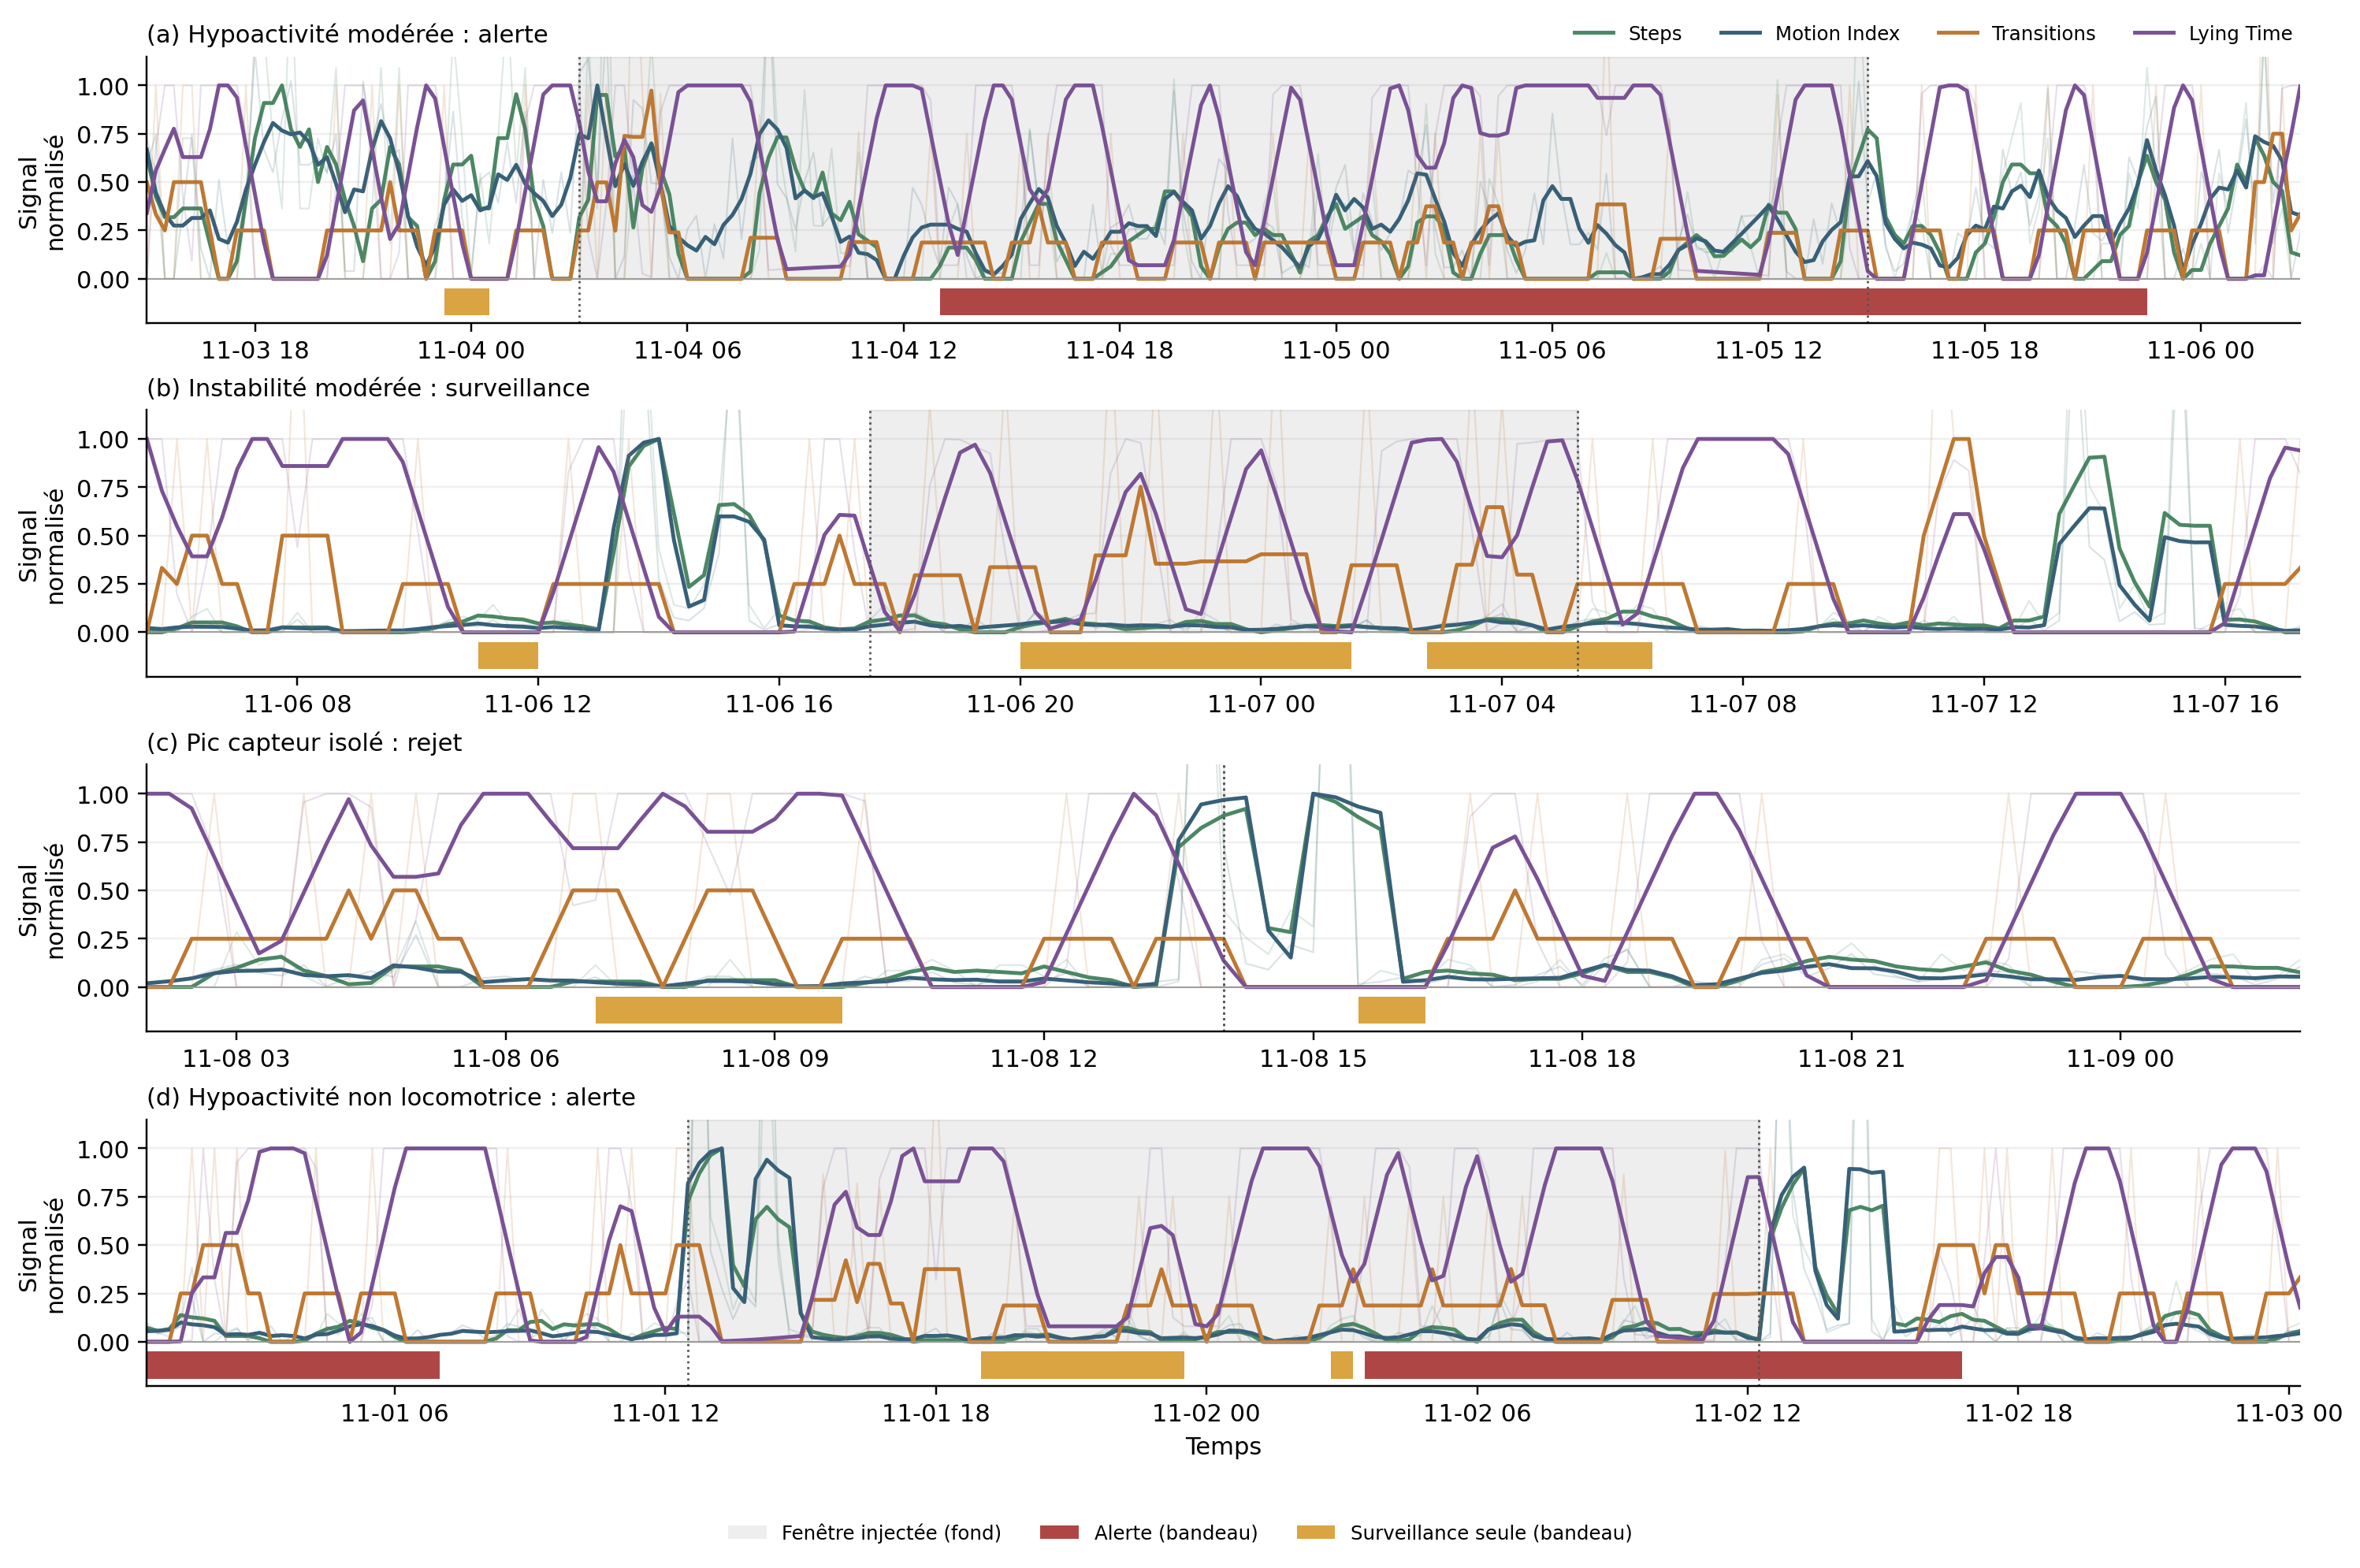
\includegraphics[width=0.95\linewidth]{figures/manual_review.png}
    \caption{Inspection visuelle de scénarios représentatifs.}
    \label{fig:manual_review}
  \end{figure}
\end{landscape}

\subsection{Calibration individuelle exploratoire}
Une calibration simple a été testée pour répondre à la variabilité du fond entre vaches.
Pour chaque vache, le seuil de 0,12 est multiplié par le rapport entre l'écart-type de son
score pendant la période de référence et la médiane de ces écarts-types. Les facteurs, estimés sans utiliser la
période future, restent compris entre 0,98 et 1,03. La procédure laisse inchangés le fond
moyen (0,402 notification par vache-jour), son coefficient de variation inter-vache (0,244)
et la couverture attribuable (87,9\,\%). Le taux de nouveaux départs passe de 57,6 à
60,6\,\%, mais IoU20 diminue de 39,4 à 33,3\,\%. Cette calibration n'apporte donc aucun gain
opérationnel et dégrade la localisation; elle n'est pas retenue. Ce résultat nul ne démontre
pas qu'aucune calibration individualisée soit possible, seulement que la dispersion du
score de référence n'est pas une base utile dans cette campagne.

\subsection{Temps d'exécution}
L'évaluation complète inclut les variables, IF, les règles IF comparatives, HYPO,
INSTABILITÉ, la fusion et la concaténation des sorties. Sur les 28 vaches et 37\,839 lignes,
la médiane de cinq répétitions est de 10,64 secondes, avec une étendue de 10,58 à 10,83
secondes et un débit médian de 3\,557 lignes par seconde. Dans le temps instrumenté, IF
représente 82,8\,\%, les variables 8,2\,\%, HYPO+INSTABILITÉ+fusion 6,4\,\% et les règles IF
comparatives 2,5\,\%. L'extension hybride ajoute donc un coût mesurable mais secondaire par rapport
au comparateur IF. Ces valeurs décrivent la machine de test et ne constituent pas un test de
charge en ferme.

Cette section établit le résultat principal du mémoire~: après soustraction de l'exécution
propre, 29 des 33 dégradations graduelles injectées sont recouvertes, 19 donnent lieu à un
nouvel épisode, et la charge de fond reste sous une notification par vache-jour.

% =====================================================================
\section{Comparaison à IF et LOF, et ablation par le comparateur pédométrique}
% =====================================================================
Les cinq variantes d'ablation sont évaluées sur les mêmes 44 fenêtres. La colonne de détection
attribuable retient le critère de nouveau départ, c'est-à-dire l'apparition d'un épisode
absent de l'exécution propre. La cinquième variante, le comparateur pédométrique, restreint
le détecteur au seul canal des pas, à la manière d'un podomètre. Le
Tableau~\ref{tab:hypo_ablation} rapporte les métriques attribuables des cinq variantes. Le
F1 événementiel y oppose les 33 dégradations graduelles, traitées comme positifs, aux
11 contrôles brefs, traités comme négatifs, sur le critère de nouveau départ attribuable.

\begin{table}[H]
  \centering
  \caption{Ablation attribuable du module HYPO.}
  \label{tab:hypo_ablation}
  \small
  \begin{tabular}{lrrrrr}
    \toprule
    Variante & Nouv. départ & IoU20 & IoU moyen & Fond/vache-jour & F1 \\
    \midrule
    A. HYPO temporel multivarié & 43,2\,\% & 29,5\,\% & 0,137 & 0,402 & 0,73 \\
    B. IF + règles de persistance & 15,9\,\% & 0,0\,\% & 0,004 & 0,152 & 0,35 \\
    C. IF ponctuel & 13,6\,\% & 0,0\,\% & 0,002 & 7,658 & 0,31 \\
    D. LOF + règles & 15,9\,\% & 0,0\,\% & 0,005 & 0,107 & 0,35 \\
    E. Comparateur pédométrique (pas seuls) & 27,3\,\% & 31,8\,\% & 0,141 & 0,518 & 0,53 \\
    \bottomrule
  \end{tabular}
\end{table}

La colonne IoU20 se lit avec le reste du tableau~: le comparateur pédométrique y devance
légèrement le détecteur complet, mais il ouvre moins de nouveaux départs et produit davantage
de fond. Les deux localisent en réalité de
façon équivalente, comme le confirme plus loin l'écart d'IoU attribuable par vache.

La dernière colonne résume la détection et le rejet des contrôles en un F1 événementiel: HYPO atteint
0,73 (IC95 par vache [0,60~; 0,86]), nettement au-dessus d'IF et de LOF (au plus 0,35). Comme
aucun contrôle n'est alerté (précision de 1,0), ce F1 ne fait toutefois que réexprimer le rappel
et n'intègre pas la charge de fond: avec la couverture attribuable, plus permissive que le
nouveau départ, le comparateur pédométrique passerait même devant HYPO sur ce seul résumé, au
prix d'un fond bien plus élevé. Le
F1 reste donc un complément des métriques décomposées et de la charge de fond, qui demeurent
privilégiées.

Après agrégation par vache, HYPO obtient un IoU supérieur aux trois variantes fondées sur IF
et LOF, soit B, C et D
($p=0{,}00098$ pour les trois comparaisons appariées de Wilcoxon~\citep{wilcoxon1945individual}).
Son taux de nouveau départ est également supérieur à B et D ($p=0{,}04297$) et à C
($p=0{,}01562$); ces valeurs sont non corrigées. Après correction de Holm pour les trois
comparaisons, l'avantage d'IoU demeure significatif dans chaque cas ($p_{aj.}=0{,}00294$).
Pour le nouveau départ, seule la comparaison avec C demeure juste sous le seuil
($p_{aj.}=0{,}04686$), tandis que celles avec B et D ne le franchissent plus
($p_{aj.}=0{,}08594$). Ces comparaisons secondaires sont donc interprétées comme
exploratoires. L'avantage est aussi de
\emph{taille}~: l'écart d'IoU attribuable moyen par vache vis-à-vis des comparateurs IF et LOF
est d'environ 0,13 (IC95 [0,106~; 0,161] contre B, [0,107~; 0,163] contre C, [0,103~; 0,161]
contre D, tous excluant zéro), avec une corrélation rang-bisériale appariée
\citep{kerby2014simple} de $+1{,}00$~:
les onze vaches favorisent HYPO. La supériorité ne tient donc pas à quelques vaches.

Cette supériorité appelle une objection, car l'analyse de sensibilité de la
Section~\ref{sec:sensibilite} fait varier 10 paramètres de HYPO et aucun paramètre des
comparateurs. Le paramètre \texttt{contamination} d'Isolation Forest et de LOF, que le
Chapitre~\ref{chapitre:etatart} désigne comme critique pour ces deux méthodes, reste figé à
0,06. L'échec de localisation des comparateurs pourrait donc refléter ce choix plutôt que
leur principe. L'ablation a été rejouée à cinq valeurs de contamination, de 0,02 à 0,15, sur
les mêmes onze vaches et les mêmes quarante-quatre événements. Aucune de ces valeurs ne
permet à B, C ou D d'atteindre le seuil IoU20 sur un seul événement, et leur IoU attribuable
moyen ne dépasse jamais 0,008, contre 0,137 pour HYPO. Ce que la contamination gouverne est
le volume d'alertes et non la localisation~: la charge de fond d'Isolation Forest ponctuel
passe de 2,509 à 14,707 notifications par vache-jour sur cette plage, sans qu'aucun événement
ne soit mieux situé. La valeur retenue ne désavantage donc pas les comparateurs, et l'écart
mesuré tient à la nature de la détection plutôt qu'à un réglage. HYPO et le comparateur
pédométrique, qui n'emploient pas Isolation Forest, restent inchangés sur toute la plage et
servent de témoin à cette vérification.

La cinquième variante isole le rôle de la combinaison de plusieurs signaux. Le comparateur
pédométrique (E) reprend exactement la machinerie temporelle de HYPO (même période de référence
individuelle par créneau horaire, même cumul CUSUM et même persistance), mais restreint la
détection au seul canal des pas, à la manière du comptage d'activité d'un podomètre
\citep{alsaaod2012electronic}; la cohérence entre familles, qu'un canal unique ne peut
satisfaire, y est relâchée pour ne pas le désavantager. Partageant cette machinerie, E
\emph{localise} les épisodes aussi précisément que le détecteur complet~: l'écart d'IoU
attribuable par vache n'est que de $-0{,}004$ (IC95 [$-0{,}032$~; 0,022], $p=0{,}966$, six
vaches sur onze le favorisant légèrement), là où les comparateurs IF et LOF s'effondrent à
un IoU quasi nul. Sa faiblesse est ailleurs~: restreint aux pas, il ouvre moins de nouveaux
    départs attribuables (27,3 contre 43,2~\%) et laisse passer davantage de fond (0,518 contre
    0,402 notification par vache-jour). Le test apparié sur la détection vaut $p=0{,}0625$ et
    n'atteint donc pas le seuil de significativité, mais cette valeur doit se lire avec la
    résolution du test~: chaque vache ne portant que quatre événements, son taux de détection ne
    peut prendre que cinq valeurs, six vaches sur onze sont à égalité exacte et l'effectif
    informatif tombe à cinq paires. Le plancher du test exact bilatéral y vaut précisément
    0,0625, de sorte que cette comparaison ne peut pas être significative à 5~\%, quelle que soit
    l'ampleur de l'écart. Les cinq paires informatives favorisent toutes HYPO. La conclusion
    prudente est donc que la supériorité en détection n'est pas établie faute de résolution, et
    non qu'elle est infirmée. L'écart pédomètre moins HYPO sur le fond atteint 0,116
    notification par vache-jour (IC95 [0,045~; 0,187]); huit vaches sur onze présentent moins de
    fond avec HYPO et le test exact apparié bilatéral vaut $p=0{,}02344$. Cette comparaison de
    fond, ajoutée après examen des autres métriques et non corrigée pour leur multiplicité, reste
    exploratoire. Elle soutient néanmoins une hypothèse utile~: plusieurs signaux pourraient
    réduire la charge de revue sans améliorer la localisation. Elle ne suffit pas à démontrer un
    avantage indépendant de la cohérence multivariée. Ce constat rejoint la limite connue des
approches strictement podométriques, dont la sensibilité dépend du seul comptage de pas
\citep{alsaaod2012electronic,oleary2020accelerometers}.

L'ablation situe donc l'apport du détecteur~: la machinerie temporelle explique l'essentiel de
l'écart avec IF et LOF, tandis que la cohérence multivariée se traduit d'abord par une charge
de vérification plus faible que celle du comparateur pédométrique.

% =====================================================================
\section{Analyses de sensibilité}
% =====================================================================
Les analyses réunies dans cette section examinent la dépendance des conclusions aux familles de signaux
retenues puis aux valeurs de paramètres. Elles évaluent une robustesse locale et ne
sélectionnent aucune nouvelle configuration.

\subsection{Apport de chaque famille de signaux}
Le comparateur pédométrique suggère, pour les pas, que la combinaison de signaux peut réduire la
charge de fond sans changer la localisation. On examine si ce motif descriptif se retrouve
en rejouant la même ablation, mais en restreignant tour à tour le détecteur à chacune
des quatre familles, comme le montre le Tableau~\ref{tab:hypo_channels}. Là où le
Tableau~\ref{tab:hypo_ablation}
situe HYPO face à d'autres familles d'algorithmes (IF, LOF, podomètre), celui-ci décompose ce
qu'il doit à chacune de ses propres familles de signaux; les deux se lisent donc ensemble.
Dans ce test, le détecteur temporel est restreint à un seul canal et la cohérence
multi-familles est relâchée. Le canal des pas correspond au comparateur pédométrique déjà
rapporté comme variante~E du Tableau~\ref{tab:hypo_ablation}.
Chaque canal porte effectivement du signal, et certains,
pris isolément et libérés de la contrainte de cohérence, ouvrent même davantage de nouveaux
départs que le détecteur complet~: les transitions seules atteignent 50,0\,\% (F1 de 0,80) et
le \textit{Motion Index} seul 34,1\,\%. Cette détection brute plus élevée se paie toutefois
exactement où on l'attend, en charge de fond~: les trois canaux d'activité isolés notifient
entre 0,49 et 0,52 fois par vache-jour, contre 0,40 pour HYPO. La posture seule illustre
l'écueil inverse~: son fond est le plus bas (0,384), mais elle ne localise presque rien
(IoU20 de 2,3\,\%). Aucune
famille ne domine donc sur tous les plans. Dans cette campagne, combiner les quatre obtient une
charge de fond basse à localisation comparable et évite de faire dépendre la décision d'un signal
unique susceptible d'être confondu, par exemple les pas gonflés par l'exercice ou l'œstrus. Ce
profil est compatible avec un gain de robustesse par cohérence, mais la résolution insuffisante du
test de détection face au comparateur pédométrique empêche de l'établir comme effet causal
indépendant~: l'écart y va constamment dans le même sens sans pouvoir être certifié.

\begin{table}[H]
  \centering
  \caption{Ablation par famille de signaux.}
  \label{tab:hypo_channels}
  \small
  \begin{tabular}{lrrrrr}
    \toprule
    Canal isolé & Nouv. départ & IoU20 & IoU moyen & Fond/vache-jour & F1 \\
    \midrule
    Pas seuls & 27,3\,\% & 31,8\,\% & 0,141 & 0,518 & 0,53 \\
    Motion Index seul & 34,1\,\% & 25,0\,\% & 0,135 & 0,491 & 0,63 \\
    Transitions seules & 50,0\,\% & 27,3\,\% & 0,128 & 0,518 & 0,80 \\
    Posture seule & 27,3\,\% & 2,3\,\% & 0,042 & 0,384 & 0,53 \\
    HYPO (quatre familles) & 43,2\,\% & 29,5\,\% & 0,137 & 0,402 & 0,73 \\
    \bottomrule
  \end{tabular}
\end{table}

Le calcul de cette ablation par canal est reproductible par
\path{scripts/compute_channel_ablation.py}. Chaque variante retire les autres familles du
score et de l'évidence cumulée par le CUSUM; la ligne « posture seule » ne conserve donc
aucune contribution cachée des pas, du \textit{Motion Index} ou des transitions.

Prises ensemble, les deux ablations (Tableaux~\ref{tab:hypo_ablation} et~\ref{tab:hypo_channels})
soutiennent surtout l'apport de la direction du changement et de la persistance. Elles font de la
cohérence entre signaux une hypothèse crédible de réduction du fond, sans démontrer son apport
indépendant sur la détection ou la localisation. Elles ne résolvent pas la charge opérationnelle,
qui reste supérieure à celle des variantes B et D.

\subsection{Robustesse locale des paramètres HYPO}
\label{sec:sensibilite}
L'analyse OFAT comprend la référence et 20 variantes de paramétrage dans lesquelles un
seul des dix
paramètres est modifié. Les 924 évaluations événement-configuration rejettent toutes le
contrôle bref. Sur les profils progressifs, 12 variantes sur 20 reproduisent exactement le
taux de nouveaux départs de la référence et 15 restent dans un écart maximal de 6,1 points.
Pour IoU20, 15 variantes restent dans un écart maximal de 3,0 points. Sur l'ensemble des
valeurs testées, le taux de nouveaux départs varie de 45,5 à 66,7\,\%, la couverture de
63,6 à 90,9\,\%, IoU20 de 27,3 à 45,5\,\%, le délai médian de 15,5 à 24,5 heures et le fond
de 0,187 à 0,553 notification par vache-jour.

La Figure~\ref{fig:hypo_sensitivity} représente l'amplitude maximale de ces écarts. Elle
mesure une influence locale des paramètres, et non une amélioration ou une optimisation de
la configuration de référence. Le panneau~(a) rapporte l'amplitude des écarts sur les
événements progressifs, le panneau~(b) celle observée sur la charge de fond. Le
Tableau~\ref{tab:hypo_sensitivity} en détaille les plages
signées pour les paramètres les plus structurants.

\begin{figure}[H]
  \centering
  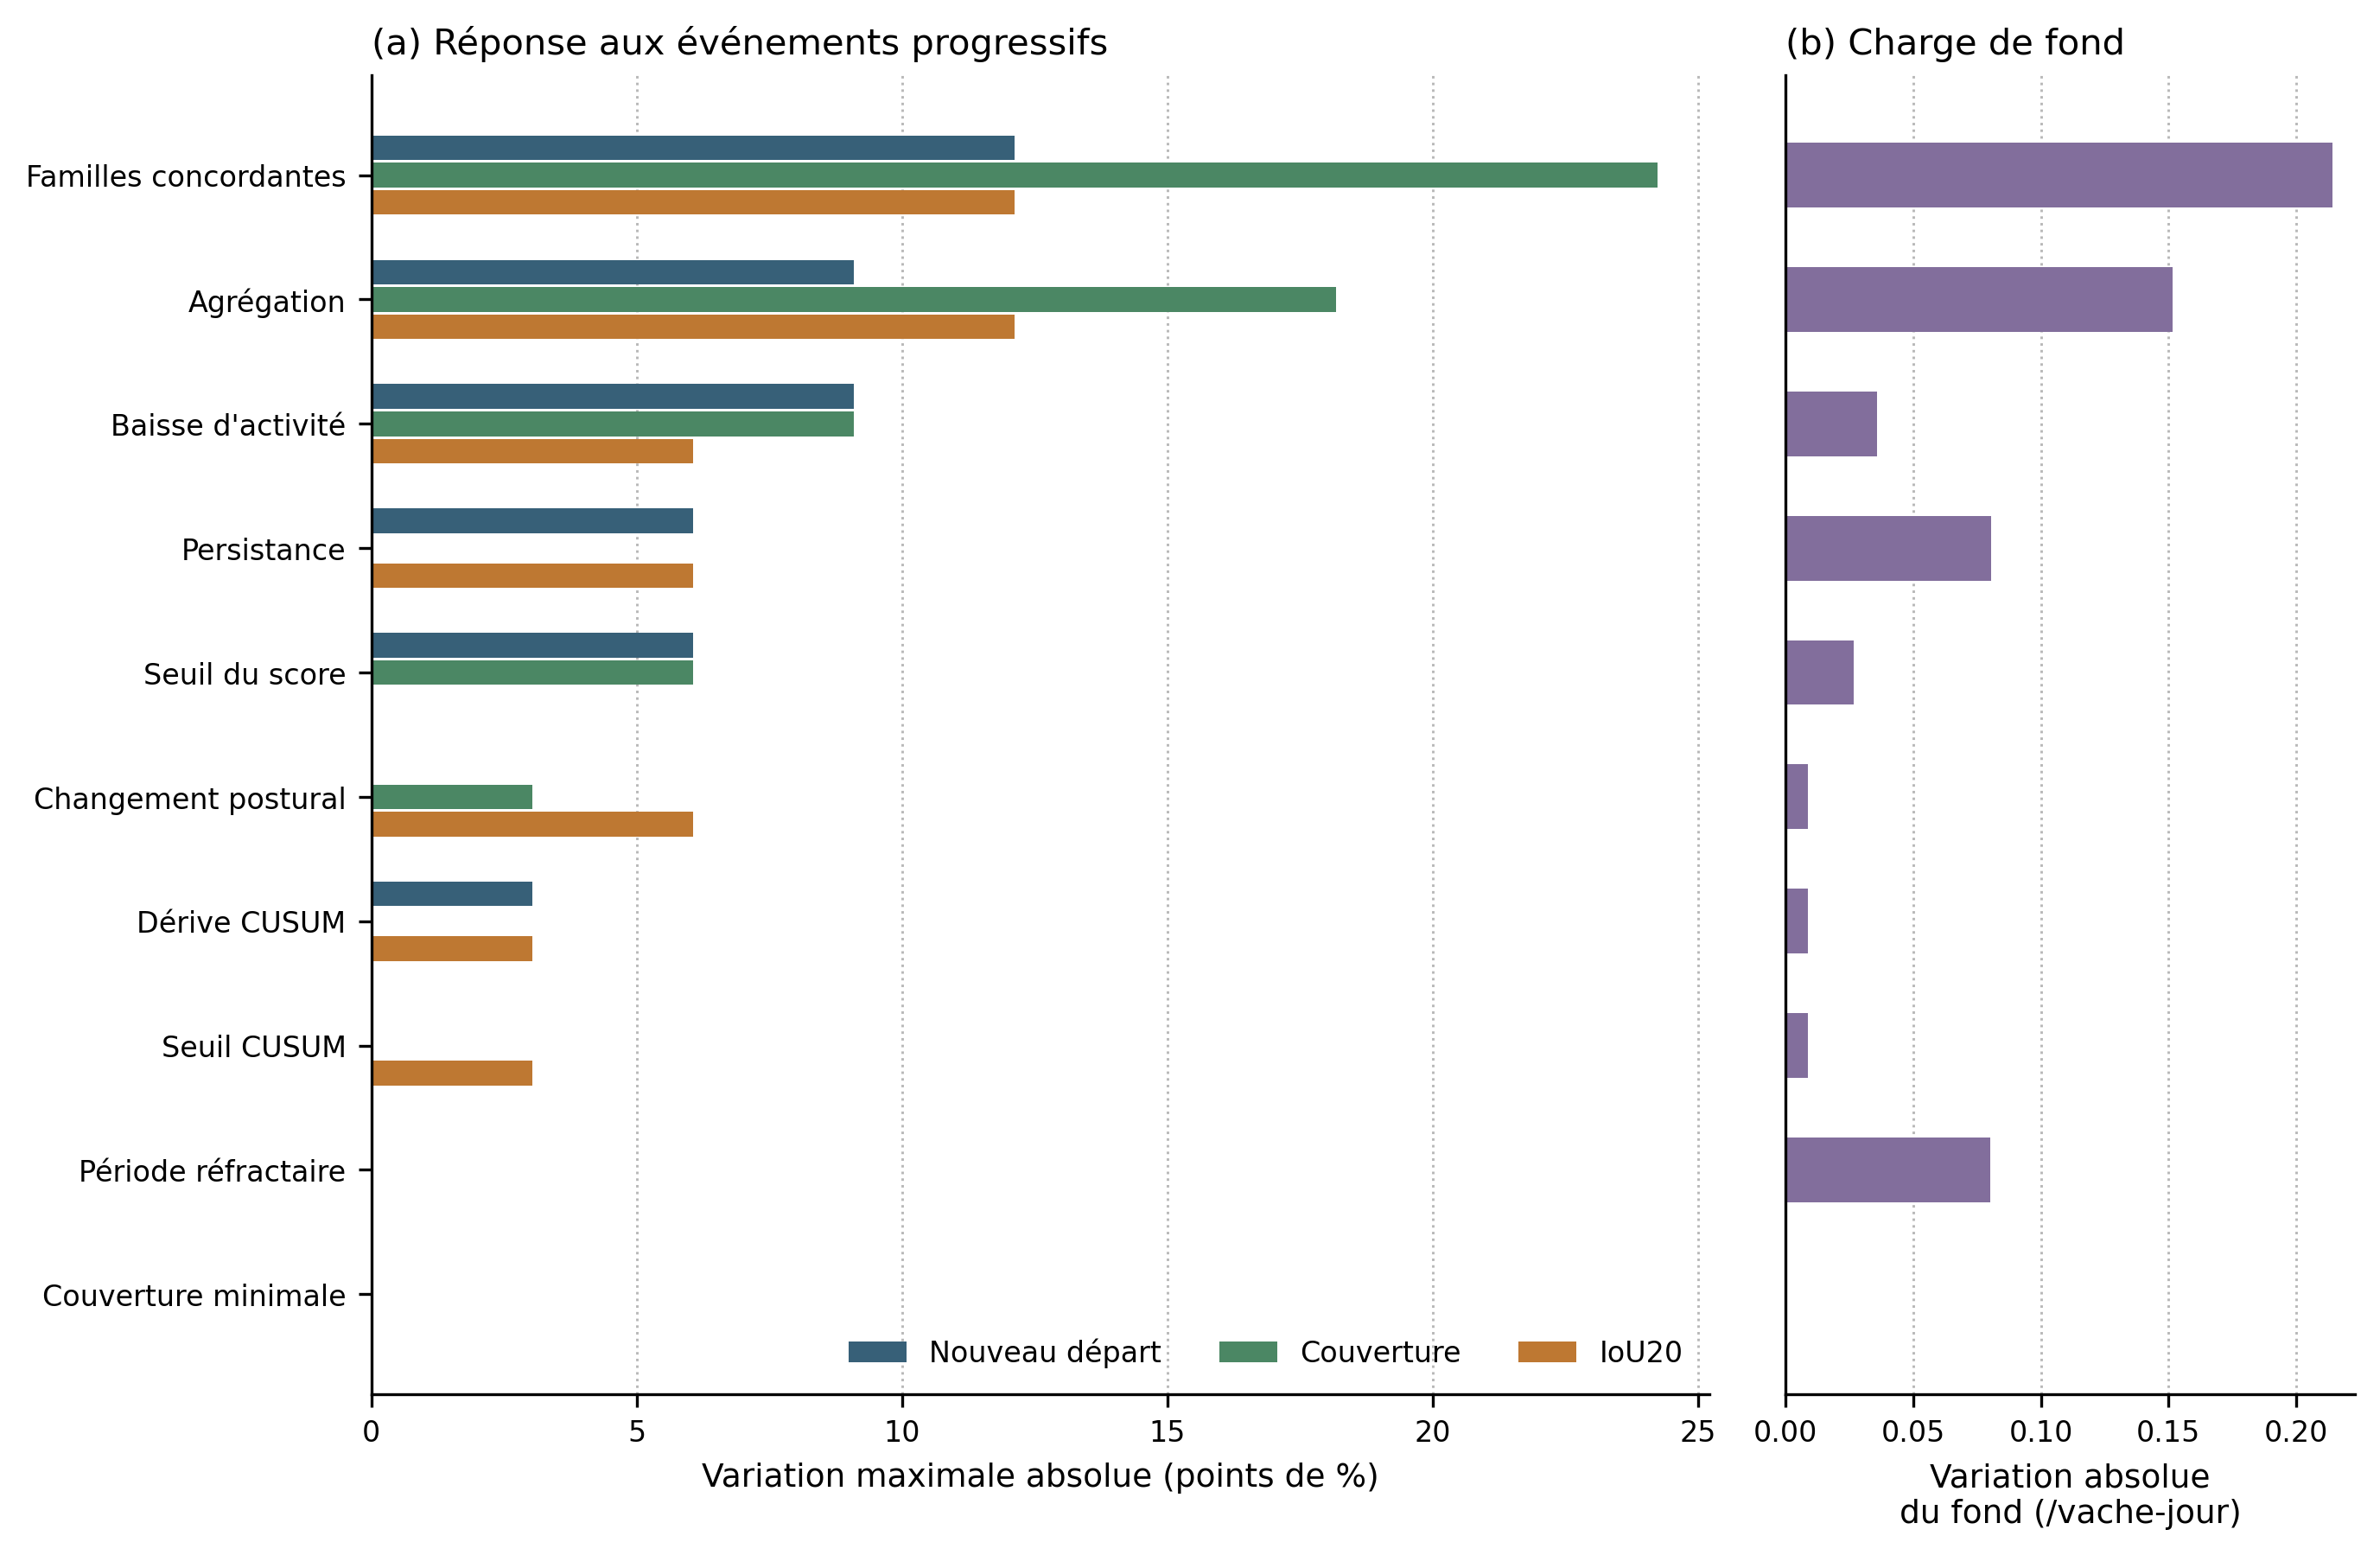
\includegraphics[width=0.98\textwidth]{figures/hypo_parameter_sensitivity_effects.png}
  \caption{Sensibilité locale des paramètres HYPO.}
  \label{fig:hypo_sensitivity}
\end{figure}

\begin{table}[H]
  \centering
  \caption{Plages d'écarts signés pour les paramètres HYPO les plus structurants.}
  \label{tab:hypo_sensitivity}
  \small
  \setlength{\tabcolsep}{3pt}
  \begin{tabular}{p{0.20\textwidth}p{0.10\textwidth}
    >{\centering\arraybackslash}p{0.13\textwidth}
    >{\centering\arraybackslash}p{0.15\textwidth}
    >{\centering\arraybackslash}p{0.12\textwidth}
    >{\centering\arraybackslash}p{0.15\textwidth}}
    \toprule
    Paramètre & Valeurs & $\Delta$ départ & $\Delta$ couverture & $\Delta$ IoU20 & $\Delta$ fond \\
      & testées & (pp) & (pp) & (pp) & (/vache-jour) \\
    \midrule
    Familles concordantes & 2; 4 & $-12{,}1$ à $0{,}0$ & $-24{,}2$ à $+3{,}0$ & $-12{,}1$ à $+3{,}0$ & $-0{,}214$ à $+0{,}107$ \\
    Agrégation & 6; 24 h & $-9{,}1$ à $+9{,}1$ & $-18{,}2$ à $0{,}0$ & $-12{,}1$ à $-3{,}0$ & $-0{,}098$ à $+0{,}152$ \\
    Baisse d'activité & 5; 15\,\% & $-9{,}1$ à $-9{,}1$ & $-9{,}1$ à $+3{,}0$ & $-6{,}1$ à $-3{,}0$ & $-0{,}036$ à $+0{,}027$ \\
    Persistance & 3; 12 h & $-6{,}1$ à $0{,}0$ & $0{,}0$ à $0{,}0$ & $-3{,}0$ à $+6{,}1$ & $-0{,}054$ à $+0{,}080$ \\
    \bottomrule
  \end{tabular}
\end{table}

Le nombre de familles et la fenêtre d'agrégation sont les choix les plus influents. Les
paramètres CUSUM et de couverture ont peu d'effet dans les plages testées. Cette stabilité
locale rend la configuration reproductible et techniquement défendable, mais ne démontre
ni son optimalité ni sa validité physiologique.

\subsection{Sensibilité des paramètres INSTABILITÉ}
Trois variantes proches sont comparées à la référence. La détection des scénarios de vérification reste entre
72,7 et 75,0\,\%, tandis que la surveillance varie de 54,5 à 66,7\,\% et le fond de 0,518 à
0,571 notification par vache-jour. Une persistance de trois heures réduit la surveillance
et augmente les confusions; une agrégation de quatre heures réduit également la surveillance.
Cette analyse soutient la stabilité locale de l'extension, mais elle est beaucoup moins
complète que l'OFAT de HYPO et ne valide pas les seuils physiologiquement.

Sur l'ensemble des 20 variantes, le contrôle bref reste rejeté sans exception~: la conclusion
de la campagne principale ne dépend donc pas d'un seuil isolé.

% =====================================================================
\section{Stress test HYPO à aire d'enveloppe appariée}
% =====================================================================
La campagne gelée applique six formes à trois positions chez chacune des onze vaches, soit
198 événements physiques et 990 évaluations pour les cinq variantes. Les cinq formes
positives modifient plusieurs familles; le contrôle négatif modifie uniquement les pas.
Chaque famille perturbée reçoit une aire numérique d'enveloppe de 36 heures, identique à celle du
profil graduel modéré de référence. Ce contrôle est satisfait pour tous les événements, avec
une erreur relative maximale inférieure à $4\times10^{-16}$. Aucun paramètre du détecteur
n'est modifié après le gel du protocole. L'appariement porte sur l'enveloppe numérique; il ne
garantit pas une variation comportementale physique identique entre vaches ou entre familles.

\begin{table}[H]
  \centering
  \caption{Réponse de HYPO aux formes moins favorables à aire d'enveloppe appariée.}
  \label{tab:hypo_stress}
  \small
  \begin{tabular}{lrrrr}
    \toprule
    Forme & $n$ & Couverture (\%) & Nouveau départ (\%) & IoU20 (\%) \\
    \midrule
    Départ abrupt & 33 & 93,9 & 54,5 & 27,3 \\
    Familles désynchronisées & 33 & 100,0 & 72,7 & 30,3 \\
    Récupération asymétrique & 33 & 93,9 & 63,6 & 21,2 \\
    Graduel bruité & 33 & 97,0 & 66,7 & 51,5 \\
    Bloc manquant de 12 h & 33 & 100,0 & 100,0 & 24,2 \\
    Pas seuls (contrôle) & 33 & 78,8 & 30,3 & 0,0 \\
    \bottomrule
  \end{tabular}
\end{table}

Le Tableau~\ref{tab:hypo_stress} détaille la réponse forme par forme.
Sur les 165 événements positifs, la moyenne des cinq taux par forme atteint 97,0\,\% de
couverture attribuable, 71,5\,\% de nouveaux départs et 30,9\,\% à IoU20. HYPO conserve
donc une forte couverture lorsque la forme s'écarte du profil graduel concordant, mais sa
localisation demeure modeste et varie selon la forme. Le bloc de données manquantes ne doit
pas être interprété comme favorable en soi: la métrique de couverture crédite tout
recouvrement attribuable, alors qu'IoU20 reste à 24,2\,\%.

\begin{table}[H]
  \centering
  \caption{Comparaisons appariées sur les cinq formes positives du stress test.}
  \label{tab:hypo_stress_comparisons}
  \small
  \begin{tabular}{lrr}
    \toprule
    Comparateur & Différence de couverture & $p$ exact unilatéral \\
    \midrule
    IF + persistance & +0,842 & 0,000488 \\
    IF ponctuel & +0,527 & 0,000488 \\
    LOF + persistance & +0,703 & 0,000488 \\
    Pédométrique, pas seuls & $-0,012$ & 0,843750 \\
    \bottomrule
  \end{tabular}
\end{table}

Les tests exacts du Tableau~\ref{tab:hypo_stress_comparisons} utilisent la moyenne de chaque
vache, et non les 165 lignes comme
observations indépendantes. Portant sur onze vaches, ils disposent de $2^{11}=2048$
permutations et d'un plancher unilatéral de 0,000488~: contrairement à la comparaison de détection de la
section précédente, leur absence de conclusion face au comparateur pédométrique n'est pas un
manque de résolution. HYPO conserve un avantage net sur IF et LOF, mais aucun avantage
n'est démontré face au comparateur pédométrique doté de la même machinerie temporelle. De
plus, le contrôle pas-seuls échoue au critère principal de spécificité~: il présente un
recouvrement attribuable dans 78,8\,\% des cas et produit un nouveau départ dans 30,3\,\%.
Le côté favorable est que ces épisodes localisent mal la fenêtre~: aucun n'atteint IoU20 et
l'IoU moyen n'est que de 0,038.

La comparaison des variantes sur ce même contrôle précise toutefois la portée de cet échec.
Le comparateur pédométrique, restreint au canal perturbé, recouvre la fenêtre dans 100,0\,\%
des cas, ouvre un nouveau départ dans 57,6\,\% et atteint IoU20 dans 54,5\,\%~: il localise
donc correctement une perturbation mono-famille. Le détecteur multivarié, lui, n'y parvient
jamais. Sur les 165 événements positifs, les deux restent proches, à 97,0 contre 98,2\,\% de
recouvrement et 30,9 contre 33,9\,\% à IoU20. L'exigence de concordance entre familles ne
supprime donc pas le déclenchement sur un canal isolé, mais elle empêche de le localiser~;
c'est la seule dimension où sa contribution propre se manifeste dans ce stress test. IF et LOF
rejettent ce contrôle plus franchement, à 0,0\,\% de recouvrement pour les variantes dotées de
règles de persistance et 12,1\,\% pour IF ponctuel, mais au prix d'un recouvrement de 12,7 à
44,2\,\% seulement sur les événements positifs.

Le stress test établit ainsi une robustesse temporelle positive face aux cinq formes moins
favorables et un avantage net sur IF et LOF, tout en délimitant précisément l'apport de la
cohérence multivariée~: démontré sur la localisation d'un stimulus mono-famille, non démontré
sur le déclenchement. Avec les signaux disponibles, une vérification contextuelle reste
nécessaire.

% =====================================================================
\section{Extension bidirectionnelle exploratoire}
% =====================================================================
\subsection{Comparaison des règles de fusion}
Le Tableau~\ref{tab:fusions} compare les cinq stratégies sur 132 scénarios. La colonne
« vérification » regroupe les trois scénarios HYPO et la séquence. La surveillance mesure le
recouvrement des trois instabilités. Les facteurs confondants regroupent l'activité de type
œstrus et l'hypoactivité non locomotrice.

\begin{table}[H]
  \centering
  \caption{Comparaison exploratoire des règles de fusion sur 132 événements.}
  \label{tab:fusions}
  \small
  \begin{tabular}{lrrrrr}
    \toprule
    Configuration & Vérification & Surveillance & Confondants & IoU20 & Fond \\
     & (\%) & instabilité (\%) & alertés (\%) & (\%) & /vache-jour \\
    \midrule
    HYPO & 61,4 & 66,7 & 40,9 & 29,5 & 0,446 \\
    INSTABILITÉ & 38,6 & 66,7 & 0,0 & 0,0 & 0,875 \\
    OU & 65,9 & 66,7 & 31,8 & 11,4 & 0,982 \\
    \textbf{HIÉRARCHIQUE} & \textbf{72,7} & \textbf{66,7} & 40,9 & \textbf{29,5} & 0,571 \\
    SÉQUENTIELLE & 56,8 & 66,7 & 36,4 & 0,0 & \textbf{0,366} \\
    \bottomrule
  \end{tabular}
\end{table}

Dans cette comparaison, toutes les sorties fusionnées utilisent un délai réfractaire commun
de 12 heures. Le fond HYPO de 0,446 diffère donc du 0,402 de la campagne principale,
où la notification propre à HYPO est espacée de 24 heures. Les valeurs ne doivent pas être
comparées comme si seul l'algorithme avait changé.

La fusion hiérarchique augmente la couverture des scénarios de vérification par rapport à HYPO seul, conserve
IoU20 à 29,5\,\%, mais élève le fond de 0,446 à 0,571. Sa fonction d'utilité technique reste
négative ($-0{,}088$), car les pénalités de confusion et de charge sont importantes. Elle est
retenue comme configuration représentative de l'extension, non comme remplacement démontré
de HYPO. La Figure~\ref{fig:fusions} compare les cinq règles de fusion.

\begin{figure}[H]
  \centering
  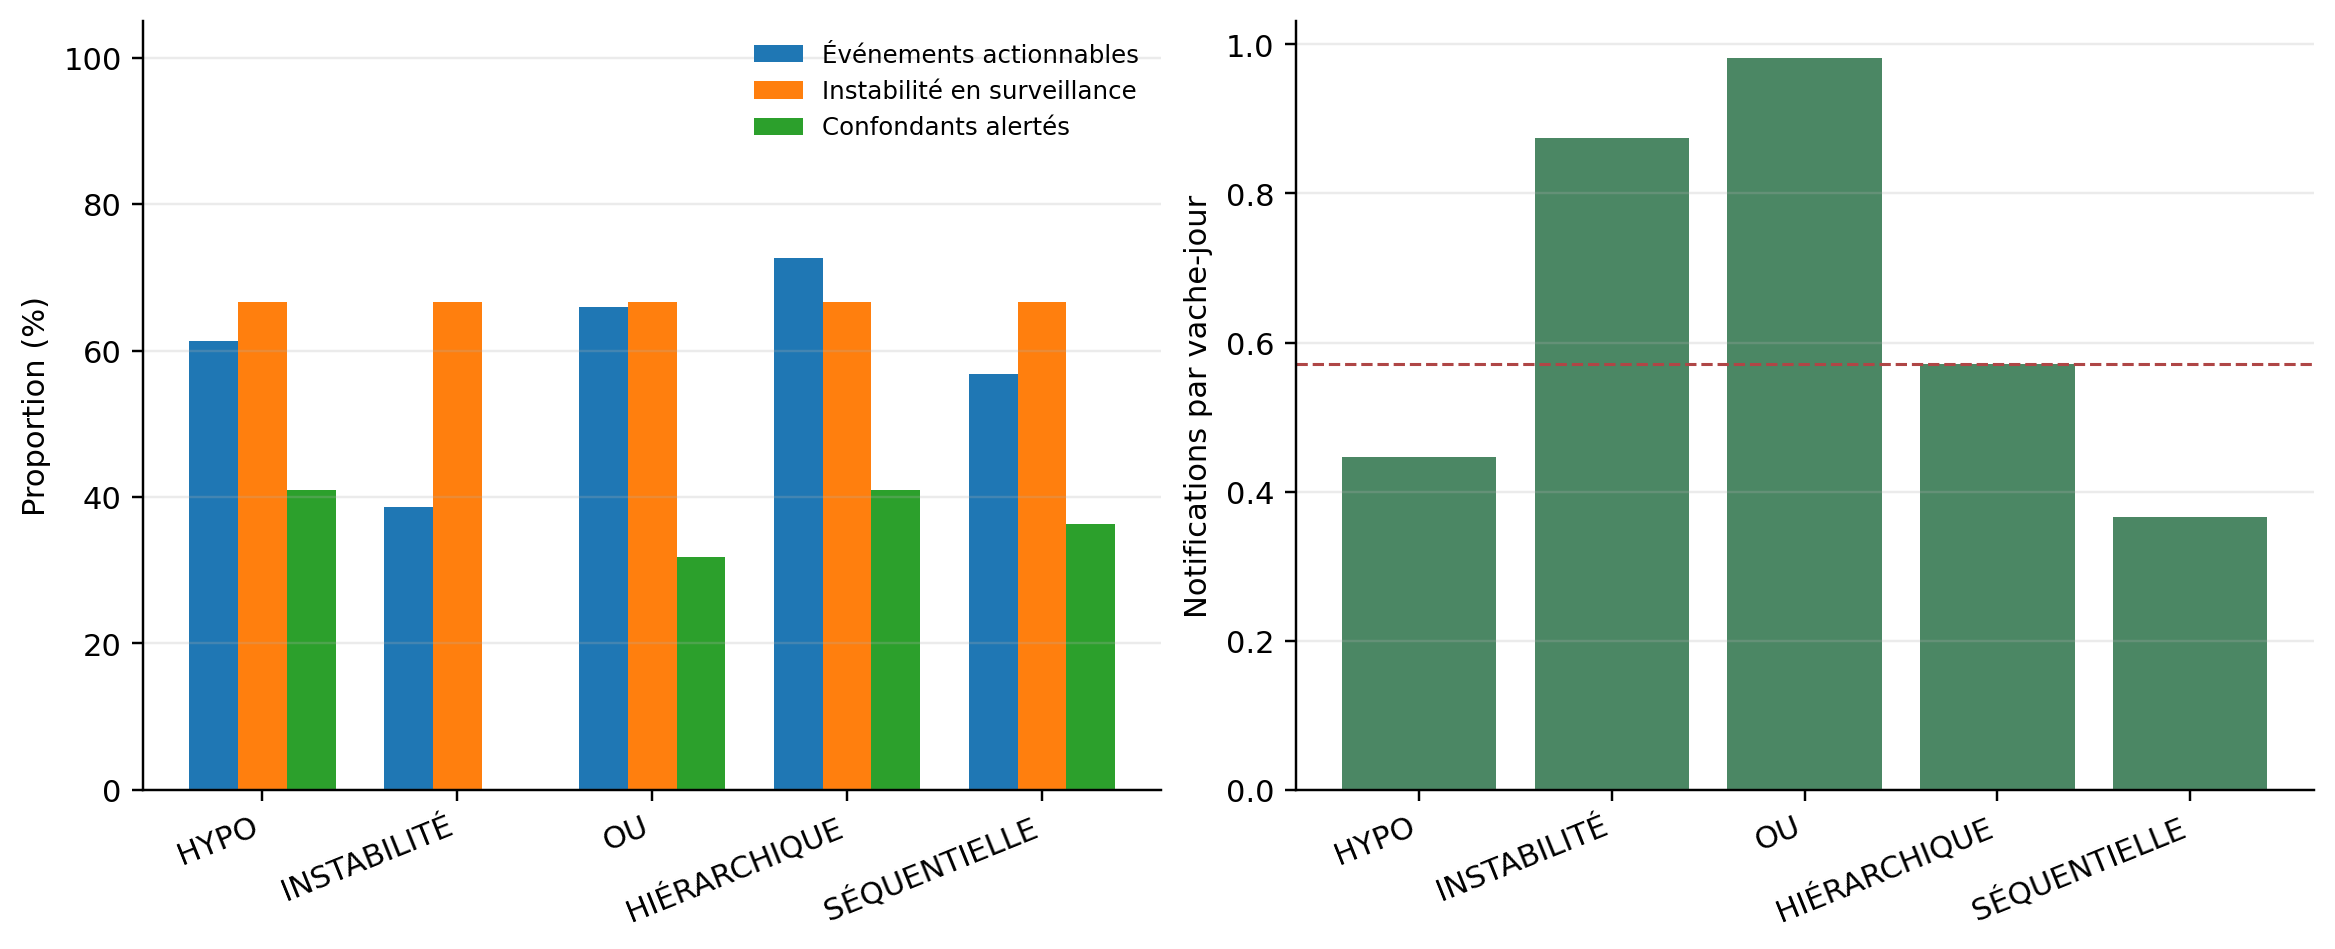
\includegraphics[width=0.92\textwidth]{figures/fusion_comparison.png}
  \caption{Comparaison des règles de fusion.}
  \label{fig:fusions}
\end{figure}

\subsection{Réponse par scénario}
La fusion hiérarchique couvre 45,5\,\% des hypoactivités légères, 72,7\,\% des modérées et
81,8\,\% des marquées. L'instabilité légère, modérée et marquée est observée en surveillance
dans respectivement 45,5\,\%, 54,5\,\% et 100,0\,\% des cas. La séquence synthétique
instabilité-hypoactivité est alertée dans 90,9\,\% des cas. Le Tableau~\ref{tab:scenarios}
détaille ces réponses par scénario, que la Figure~\ref{fig:scenarios} représente
visuellement.

\begin{table}[H]
  \centering
  \caption{Réponse de la fusion hiérarchique par scénario.}
  \label{tab:scenarios}
  \small
  \begin{tabular}{lrrr}
    \toprule
    Scénario & $n$ & Alerte de vérification (\%) & Surveillance (\%) \\
    \midrule
    Hypoactivité légère & 11 & 45,5 & 0,0 \\
    Hypoactivité modérée & 11 & 72,7 & 18,2 \\
    Hypoactivité marquée & 11 & 81,8 & 54,5 \\
    Instabilité légère & 11 & 9,1 & 45,5 \\
    Instabilité modérée & 11 & 9,1 & 54,5 \\
    Instabilité marquée & 11 & 18,2 & 100,0 \\
    Instabilité puis hypoactivité & 11 & 90,9 & 81,8 \\
    Contrôles brefs regroupés & 33 & 0,0 & 0,0 \\
    Activité de type œstrus & 11 & 0,0 & 0,0 \\
    Hypoactivité non locomotrice & 11 & 81,8 & 0,0 \\
    \bottomrule
  \end{tabular}
\end{table}

\begin{figure}[H]
  \centering
  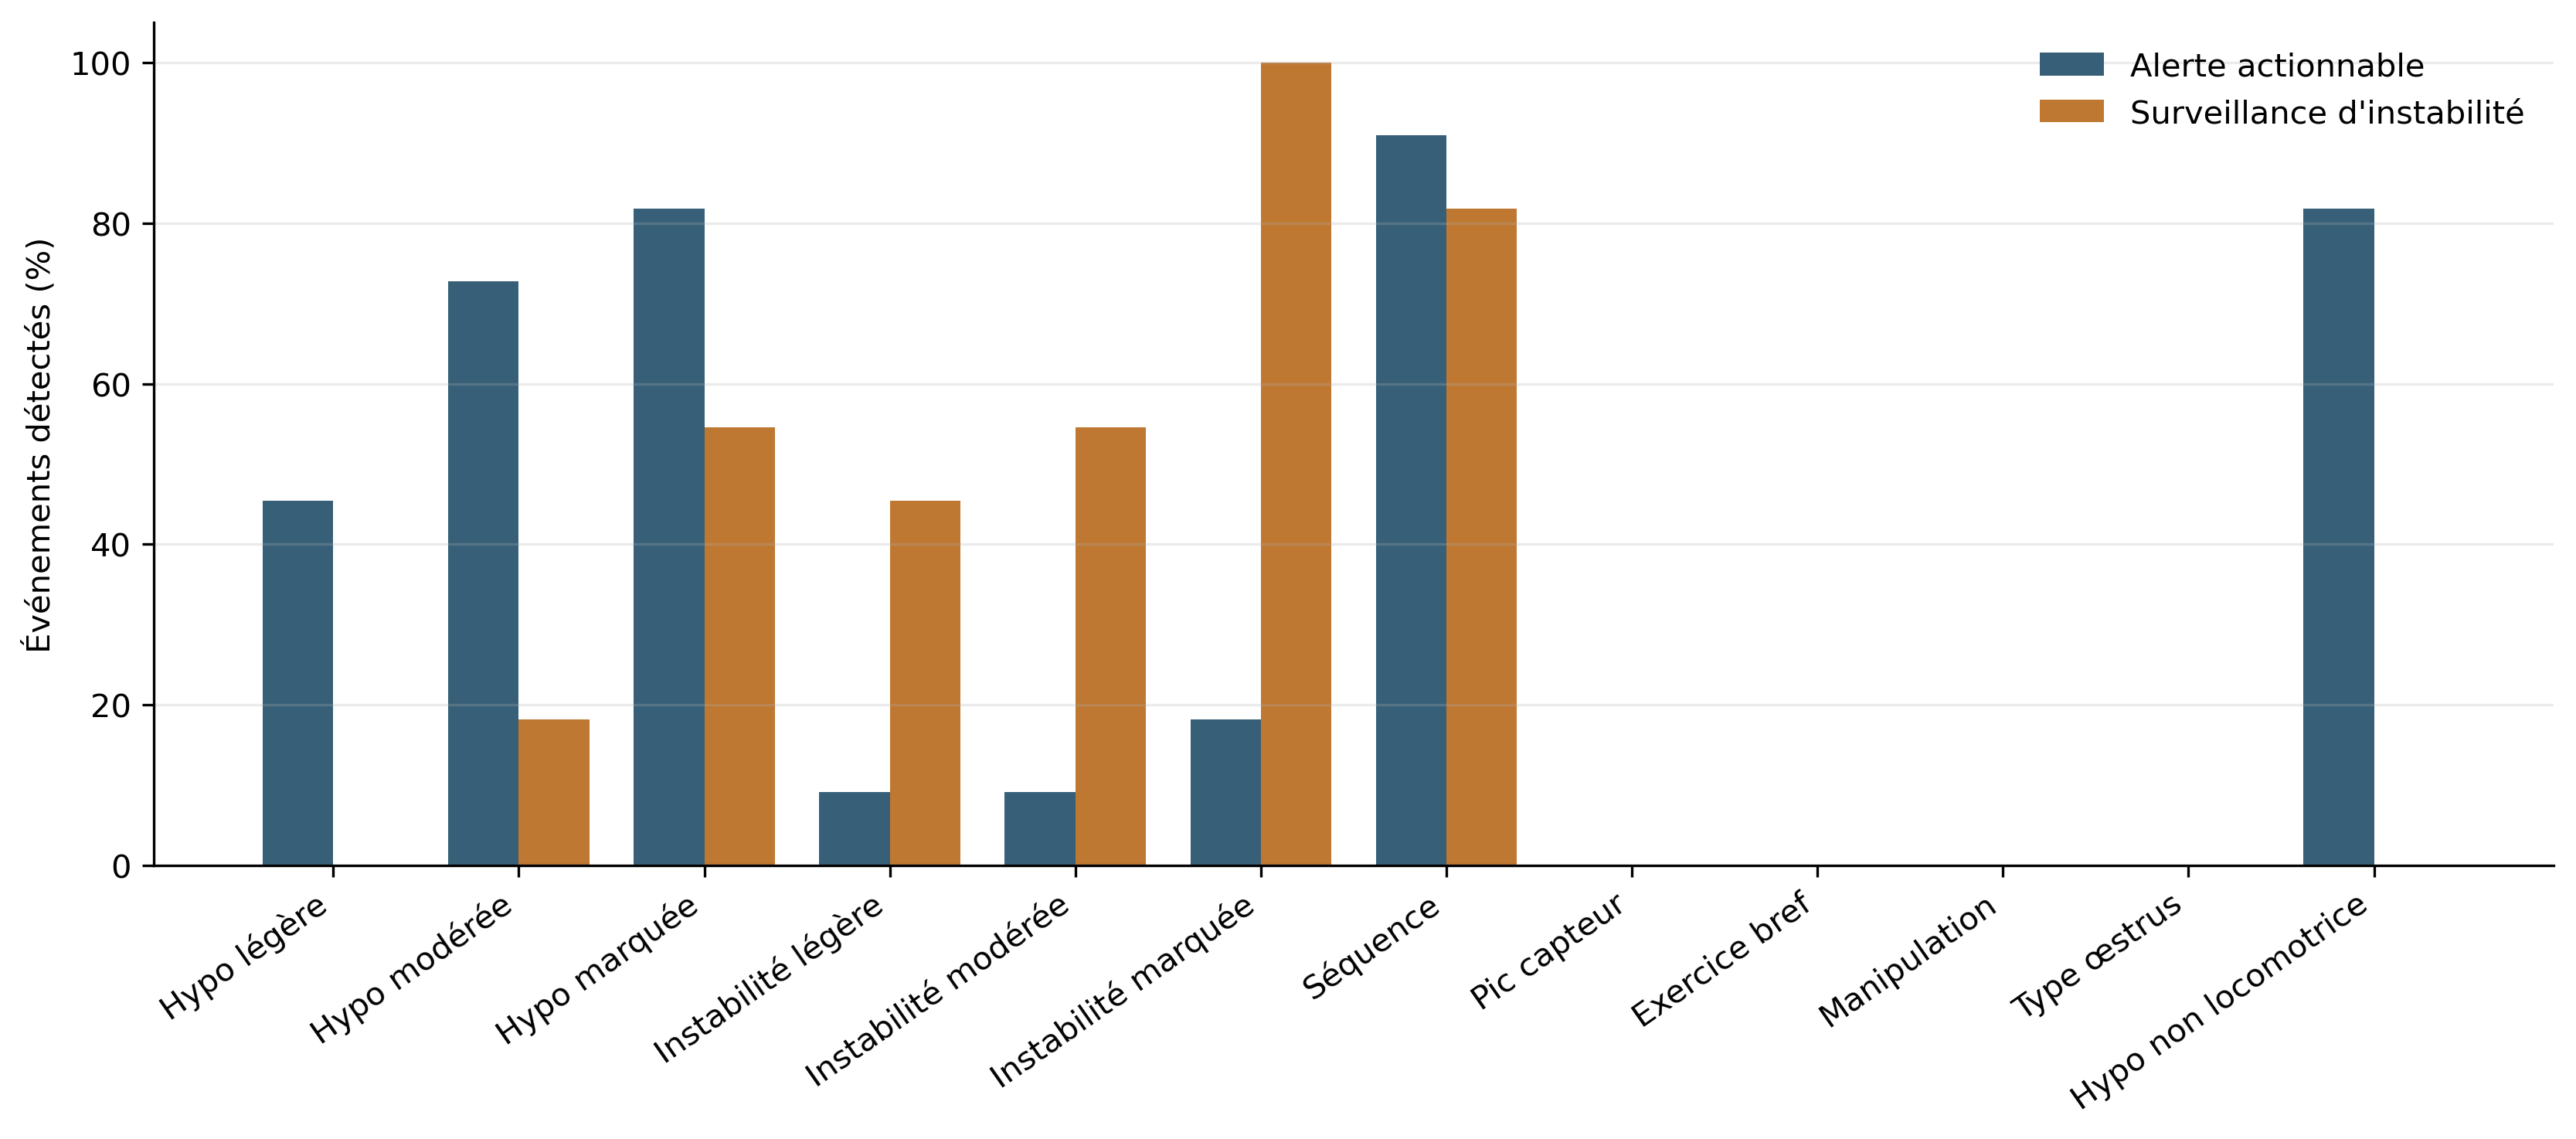
\includegraphics[width=0.94\textwidth]{figures/scenario_results.png}
  \caption{Réponse par scénario contrôlé.}
  \label{fig:scenarios}
\end{figure}

Parmi les scénarios de vérification, 29,5\,\% atteignent IoU20. Le délai médian est de
19,875 heures. Le fond hiérarchique est de 0,571 notification par vache-jour, avec une
étendue de 0,295 à 0,884 entre vaches. Aucun des 33 contrôles brefs ne produit de nouveau
départ de vérification ou de surveillance. Par ailleurs, l'alerte de neuf hypoactivités non
locomotrices sur onze démontre une limite d'identifiabilité:
des causes différentes peuvent produire la même forme sur les capteurs disponibles.

L'extension apporte ainsi une surveillance des instabilités que HYPO seul ne produit pas, sans
améliorer la localisation ni réduire la charge~: elle complète le détecteur principal plutôt
qu'elle ne le remplace.

% =====================================================================
\section{Évaluation observationnelle IceTag-SLS}
% =====================================================================
\label{sec:validation_mcgill}

Quatorze vaches sont évaluables. Les trois vaches SLS~$\geq2$ appartiennent toutes au groupe
\textit{Exercise}; aucune vache du groupe sans exercice n'atteint ce seuil. Dans les sept
jours précédant le score, la fusion hiérarchique produit en moyenne 6,67 notifications chez
les trois vaches SLS~$\geq2$, contre 4,45 chez les onze autres. L'AUC exploratoire est
0,924. L'énumération exhaustive des 364 répartitions possibles des trois étiquettes positives
donne $p=0{,}019$ en unilatéral et $p=0{,}030$ en bilatéral, en accord avec le test de
Mann-Whitney ($p=0{,}031$). La corrélation de Spearman vaut $\rho=0{,}504$ avec
$p=0{,}066$. Chaque point de la Figure~\ref{fig:sls} représente une vache; l'effectif de
trois vaches dans le groupe SLS~$\geq2$ impose une interprétation prudente.

Deux contrôles précisent ce résultat positif. D'abord, retirer successivement chacune des trois
vaches SLS~$\geq2$ maintient l'AUC globale entre 0,909 et 0,955~: le classement n'est donc pas
porté par une seule vache. Ensuite, le test max-stat exact reste favorable lorsqu'il contrôle
les cinq variantes de fusion pour la mesure de notifications ($p=0{,}0467$ en unilatéral).
Lorsqu'il englobe les vingt combinaisons variante-métrique examinées, il devient non concluant
($p=0{,}0742$ en unilatéral et $p=0{,}1236$ en bilatéral). Le signal favorable est donc
spécifique au nombre de notifications et suffisamment stable pour justifier une étude plus
grande, mais il ne constitue pas une confirmation familiale sur toutes les analyses explorées.
Ce contrôle de multiplicité ayant été ajouté après l'analyse principale, il demeure lui-même
exploratoire.

\begin{figure}[H]
  \centering
  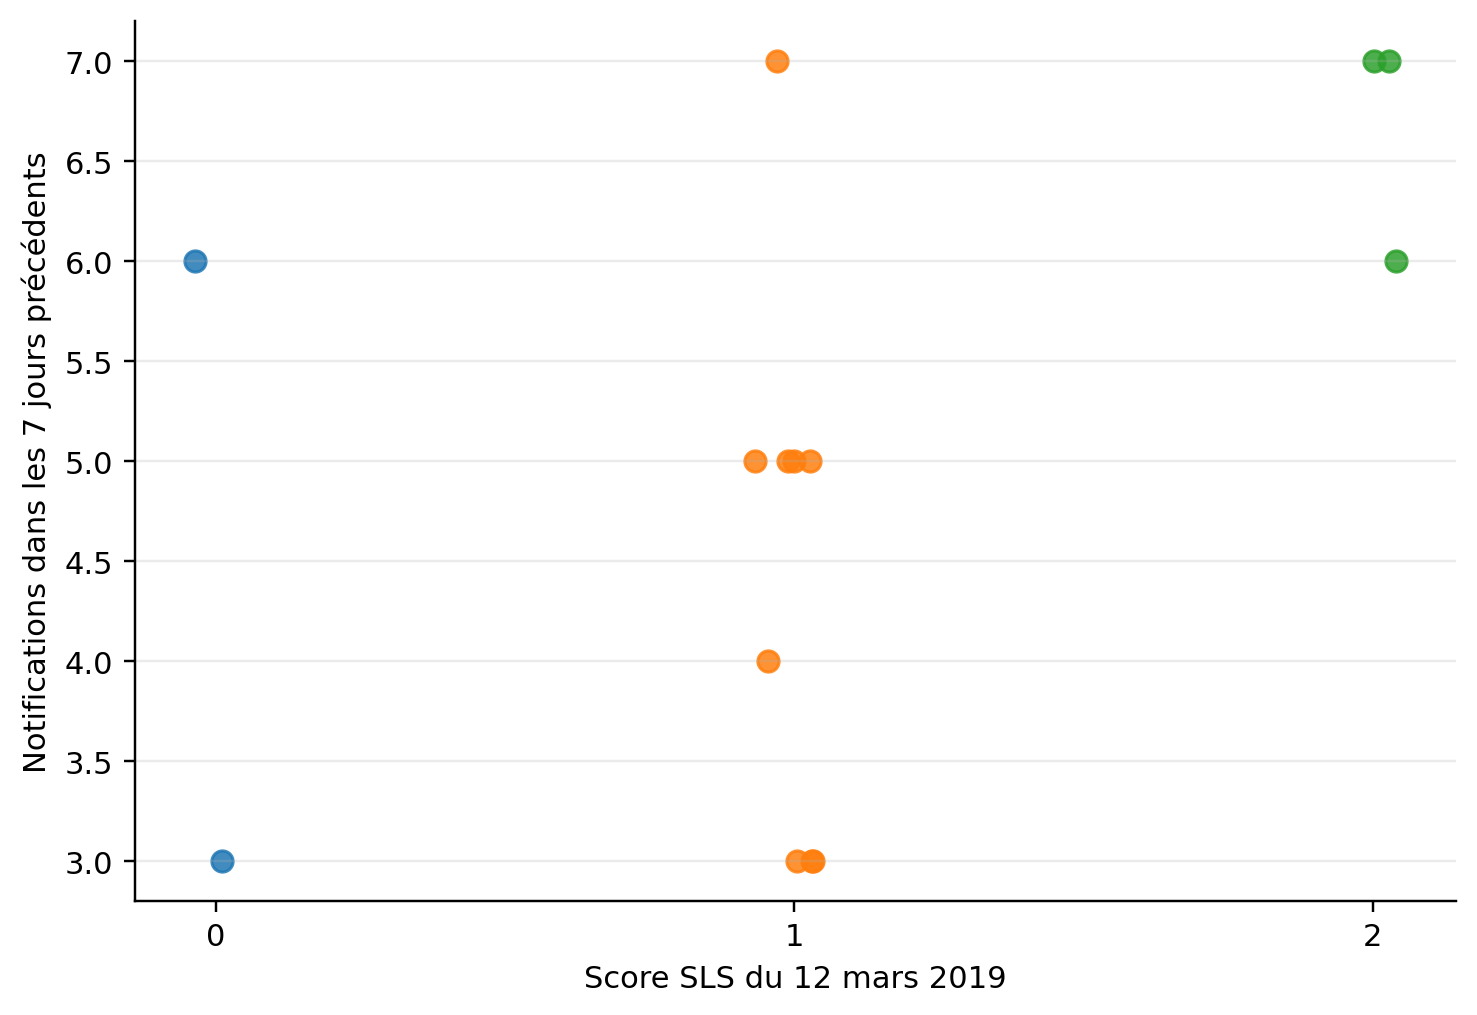
\includegraphics[width=0.72\textwidth]{figures/sls_notifications.png}
  \caption{Notifications précédant le score SLS.}
  \label{fig:sls}
\end{figure}

Les mesures secondaires sont moins séparatrices: l'AUC de la fraction du temps en épisode
est 0,712, celle du score maximum 0,606 et celle de la surveillance d'instabilité 0,348. La
charge future atteint environ 0,755 notification par vache-jour. L'ensemble forme un signal
de concordance intéressant. Cependant, les trois vaches SLS~$\geq2$ se trouvent dans le
groupe \textit{Exercise}, contre trois des dix vaches sous le seuil dont le traitement est
connu; le test exact de Fisher donne $p=0{,}070$. Dans le seul groupe
\textit{Exercise}, l'AUC reste orientée dans le même sens (0,778), mais le test exact
bilatéral est non concluant ($p=0{,}40$). Comme pour la détection face au comparateur
pédométrique, cette absence de conclusion tient d'abord à la résolution~: six vaches réparties
en trois positives et trois négatives n'autorisent que vingt permutations, et le plancher du
test exact bilatéral y vaut 0,10. Ce test ne pouvait donc pas être significatif à 5~\%. Le
groupe sans exercice ne contient aucun cas
SLS~$\geq2$, donc aucune AUC interne n'y est estimable. Malgré la stabilité du classement
global au retrait d'une vache positive, sa portée clinique demeure limitée par le petit
effectif, la multiplicité et la confusion avec le traitement.

Le classement global reste néanmoins net, avec une AUC de 0,924~: c'est la seule confrontation
à des scores locomoteurs réels dont dispose ce travail, et elle va dans le sens attendu.

% =====================================================================
\section{Correspondance entre objectifs et résultats}
% =====================================================================
Le Tableau~\ref{tab:objectifs_resultats} vérifie qu'aucun objectif annoncé dans
l'introduction ne reste sans résultat et qu'aucun résultat principal n'est introduit sans
objectif préalable.

\begin{table}[H]
  \centering
  \caption{Correspondance entre objectifs et résultats.}
  \label{tab:objectifs_resultats}
  \small
  \begin{tabular}{p{0.05\textwidth}p{0.25\textwidth}p{0.42\textwidth}p{0.13\textwidth}}
    \toprule
    Obj. & Attente & Résultat principal & Statut \\
    \midrule
    1 & Référence individuelle et chronologique
      & Séparation 60/40, référence par vache et créneau, contrôles d'intégrité conformes.
      & Réalisé \\
    2 & Détection HYPO persistante
      & 87,9\,\% de couverture attribuable et 39,4\,\% à IoU20 sur 33 profils graduels.
      & Réalisé \\
    3 & Ablation et sensibilité HYPO
      & Supériorité sur IF/LOF; OFAT de 20 variantes; forte couverture des formes de stress
        à aire d'enveloppe appariée, mais contrôle pas-seuls non rejeté sur le recouvrement.
      & Réalisé \\
    4 & Explorer INSTABILITÉ et les fusions
      & Surveillance de 22/33 instabilités; aucune supériorité de la fusion sur HYPO.
      & Exploratoire \\
    5 & Contrôles, confondants, fond et coût
      & Contrôles brefs rejetés, 9/11 hypoactivités non locomotrices alertées,
        fond HYPO de 0,402 et temps médian de 10,64~s.
      & Réalisé \\
    6 & Confrontation IceTag-SLS
      & AUC globale de 0,924; analyse interne au groupe \textit{Exercise} non concluante
        (AUC 0,778; test exact bilatéral $p=0{,}40$).
      & Exploratoire \\
    \bottomrule
  \end{tabular}
\end{table}

La campagne principale établit que HYPO transforme des baisses graduelles injectées après
la période de référence en épisodes attribuables, mieux localisés que ceux des comparateurs IF
et LOF. Le contrôle bref est rejeté, l'ablation favorise HYPO chez les onze vaches, et l'OFAT
montre que la conclusion ne dépend pas d'un seul seuil isolé. Le comparateur pédométrique
localise de façon proche, mais recouvre moins d'événements et produit plus de fond.
L'extension bidirectionnelle ajoute une surveillance utile des instabilités et récupère les
séquences synthétiques. Elle apporte une lecture complémentaire du comportement, tout en
gardant HYPO comme résultat principal. Son apport se situe dans la séparation des sorties et
dans le gain de couverture, tandis que l'IoU20 inchangé et l'augmentation de la charge de fond
définissent les priorités de son perfectionnement.


% Discussion generale et conclusion : un seul bloc en texte suivi
% =====================================================================
% Discussion generale et conclusion : texte suivi, sans intitules de
% section, conformement au plan valide. Le mecanisme reprend celui de
% l'environnement conclusion de la classe memoireuqam (chapitre non
% numerote, entree de table des matieres), avec le titre retenu.
% =====================================================================
\chapter*{DISCUSSION GÉNÉRALE ET CONCLUSION}
\addtocontents{toc}{\protect\vspace{1.5ex}}
\addcontentsline{toc}{chapter}{DISCUSSION GÉNÉRALE ET CONCLUSION}

% Ce chapitre n'etant pas numerote, le compteur de chapitre n'avance pas et
% ses tableaux heriteraient du numero du chapitre 6. On leur donne un prefixe
% propre, comme l'annexe utilise A. La numerotation par chapitre est retablie
% en fin de fichier, pour que l'annexe retrouve A.1 et suivants.
\setcounter{secnumdepth}{0}   % intitules non numerotes : \section* est
% Les intitules de ce chapitre ne portent pas de numero. Sans lui, la classe
% UQAM les compose en romain de taille normale et ils se confondent avec le
% corps du texte. Ils passent donc en italique, ici seulement : les sections
% numerotees des chapitres 1 a 6 gardent leur presentation, leur numero
% suffisant a les identifier. La definition d'origine est retablie plus bas,
% avec le compteur.
\makeatletter
\renewcommand\section{\@startsection{section}{1}{\z@}%
  {12bp\@plus.2ex\@minus.2ex}{0.01bp\@plus.2ex}%
  {\normalfont\normalsize\itshape\baselineskip=\simpleinter}}
\makeatother
                              % inoperant dans memoireuqam.cls
\setcounter{table}{0}
\renewcommand{\thetable}{D.\arabic{table}}

Ce mémoire s'est déployé en six temps. Le Chapitre~\ref{chapitre:contexte} a établi l'enjeu
économique et zootechnique de la boiterie, son étiologie multifactorielle, les limites de la
notation locomotrice conventionnelle et les variables comportementales que restituent les
capteurs portés. Le Chapitre~\ref{chapitre:etatart} a passé en revue les approches automatisées
de détection, les méthodes non supervisées de référence et la détection temporelle de
changements persistants, avant de montrer que l'hétérogénéité des protocoles interdit de
comparer directement les performances publiées. Le Chapitre~\ref{chapitre:systeme} a défini le
système proposé~: la période de référence individuelle, la branche HYPO, la branche
INSTABILITÉ, leur fusion hiérarchique, les comparateurs et le protocole d'évaluation, avec les
métriques et l'organisation logicielle qui les rendent reproductibles. Le
Chapitre~\ref{chapitre:donnees} a décrit le corpus IceQube 2023, la préparation des données et
le cadre expérimental. Le Chapitre~\ref{chapitre:interface} a présenté l'interface de
priorisation, ses trois niveaux de priorité et les limites de son usage en ferme. Le
Chapitre~\ref{chapitre:resultats} a enfin rapporté la performance attribuable du module HYPO,
sa comparaison aux détecteurs d'anomalies ponctuels, ses analyses de sensibilité, le test de
stress à aire d'enveloppe appariée, l'extension bidirectionnelle et la confrontation à la
cohorte IceTag-SLS.

\section{Contributions}
Au terme de ce travail, les contributions peuvent être résumées ainsi. Le mémoire fournit une
évaluation attribuable de HYPO avec intervalles de confiance, une ablation et ses tailles
d'effet, une analyse OFAT, une courbe reliant détection et charge, une tentative de
calibration individuelle rapportée malgré son résultat négatif, une extension bidirectionnelle
assortie de contrôles de confusion, une évaluation du temps d'exécution, une analyse SLS
synchronisée, une interface de priorisation et des artefacts reproductibles. Sa contribution
méthodologique est double~: proposer un détecteur temporel interprétable, et montrer comment
évaluer ce type d'outil sans confondre résultats techniques, hypothèses exploratoires et
interprétations cliniques. Le code source, les paramètres figés, les douze profils d'injection
et les scripts d'évaluation sont versionnés, avec un manifeste d'intégrité SHA-256 des sorties
et de l'empreinte du corpus source (Annexe~\ref{annexe:validation})~; les données capteurs brutes ne peuvent être diffusées pour
des raisons de confidentialité. Les artefacts et leurs empreintes publiés permettent d'auditer
les résultats, et la démarche complète, des injections jusqu'aux figures du manuscrit, reste
reproductible par les personnes autorisées à accéder aux données.

Le module HYPO constitue en définitive le résultat technique principal~: il démontre sa
capacité à transformer des baisses graduelles en épisodes attribuables, surpasse les variantes
IF/LOF évaluées pour la localisation et conserve une logique interprétable par vache. Sa
performance de localisation et sa charge de vérification définissent désormais des objectifs
d'amélioration mesurables.
L'extension bidirectionnelle organise une hypothèse complémentaire et quantifie ses compromis.
Cette séparation entre preuve principale et exploration rend l'ensemble cohérent et fournit
une base reproductible pour développer et évaluer un futur usage de priorisation en ferme.

\section{Ce que le système établit}
L'objectif de ce mémoire était de concevoir une chaîne reproductible qui transforme des
mesures indirectes du capteur IceQube en priorités de vérification locomotrice. Son apport central est
de montrer qu'une alerte comportementale peut être construite autour d'une trajectoire
individuelle plutôt qu'autour de points anormaux isolés. La branche HYPO combine direction du
changement, cohérence entre signaux et persistance temporelle. Cette combinaison produit
des épisodes plus cohérents avec les dégradations graduelles que les comparateurs IF
et LOF. Après soustraction de l'exécution propre, HYPO couvre 29 des 33 événements
graduels et atteint IoU20 dans 13 cas. Ce résultat établit la capacité du système à
transformer une dégradation contrôlée en priorité de vérification localisée.

Le résultat établi se lit à deux niveaux complémentaires. La couverture de 87,9\,\% montre que HYPO
réagit dans la plupart des fenêtres injectées, tandis que le taux de nouveaux départs de
57,6\,\% distingue les épisodes réellement ouverts de ceux qui prolongent une alerte déjà
active. Le délai médian de 20,75 heures situe le caractère \textit{précoce} relativement aux
dégradations de 36 à 60 heures. Ces indicateurs précisent l'usage opérationnel du système~:
prioriser une vérification lorsque plusieurs familles de signaux se dégradent de façon
persistante, avec une traçabilité suffisante pour expliquer pourquoi une vache remonte dans le
classement. Le Tableau~\ref{tab:portee_conclusions} associe chaque conclusion à son niveau de
preuve.


La comparaison de HYPO aux autres détecteurs apporte un résultat méthodologique important~: la
quantité de points anormaux n'est pas le critère décisif. IF ponctuel produit
7,658 départs par vache-jour sans atteindre IoU20 sur un seul événement, et les variantes IF
et LOF suivies de persistance réduisent la charge sans localiser davantage les fenêtres. HYPO
atteint, pour sa part, un IoU attribuable moyen de 0,137 et un taux de 29,5\,\% à IoU20 sur
les quatre profils. La direction du changement et l'accumulation temporelle sont donc mieux soutenues
que la simple accumulation d'anomalies ponctuelles. La contribution propre de la cohérence
entre familles demande toutefois une comparaison supplémentaire, car le comparateur
pédométrique partage la même machinerie temporelle.

\begin{table}[H]
  \centering
  \caption{Portée des conclusions principales.}
  \label{tab:portee_conclusions}
  \small
  \begin{tabular}{p{0.22\textwidth}p{0.34\textwidth}p{0.35\textwidth}}
    \toprule
    Niveau & Conclusion permise & Conclusion non permise \\
    \midrule
    Démontré techniquement
      & HYPO réagit à des baisses graduelles après la période de référence et localise mieux ces scénarios
        que les comparateurs IF/LOF.
      & HYPO identifie à lui seul la cause de la dégradation. \\
    Soutenu mais limité
      & Le mécanisme temporel reste robuste à cinq formes moins favorables à aire
        d'enveloppe appariée.
      & La cohérence multivariée apporte un gain démontré sur un comparateur pédométrique
        doté de la même machinerie temporelle. \\
    Exploratoire
      & INSTABILITÉ peut produire une sortie de surveillance distincte et la fusion peut
        représenter une séquence synthétique.
      & L'instabilité précède habituellement une boiterie réelle. \\
    À établir dans un protocole clinique
      & Validation longitudinale avec examens locomoteurs et causes documentées.
      & Sensibilité, spécificité, valeur prédictive ou bénéfice clinique. \\
    \bottomrule
  \end{tabular}
\end{table}

Le test de stress à aire d'enveloppe appariée apporte cette comparaison sur 5 formes moins
favorables, 3 positions et 11 vaches. Sur les 165 événements positifs, HYPO atteint en moyenne
97,0\,\% de couverture attribuable, 71,5\,\% de nouveaux départs et un taux de 30,9\,\% à
IoU20. HYPO conserve un avantage exact sur IF, IF avec persistance et LOF avec persistance
($p=0{,}000488$ pour chaque comparaison). Ce résultat positif montre que l'avantage de HYPO
sur les détecteurs ponctuels ne dépend pas uniquement de la forme graduelle initiale. En
revanche, sa couverture ne dépasse pas celle du comparateur pédométrique temporel
(différence $-0{,}012$, $p=0{,}844$), et le contrôle pas-seuls échoue au critère principal de
spécificité: 78,8\,\% de recouvrement attribuable et 30,3\,\% de nouveaux départs. Ce contrôle
reste toutefois mal localisé (IoU moyen de 0,038 et aucun événement à IoU20). La campagne
soutient donc la robustesse temporelle de HYPO aux formes moins favorables, mais ne démontre
pas un gain indépendant de spécificité multivariée.

L'analyse OFAT montre ensuite que ces conclusions ne reposent pas sur \textbf{une valeur unique} de
chaque seuil. Elle identifie toutefois deux choix structurants~: l'agrégation et le nombre de
familles concordantes. Exiger quatre familles réduit fortement la couverture et le fond, alors
que n'en exiger que deux augmente la charge~; une \textbf{agrégation courte} réagit plus vite mais
localise moins bien, tandis qu'une \textbf{agrégation longue} perd des événements. Les valeurs de
référence constituent donc un compromis documenté, non un optimum. Modifier les seuils après
lecture de cette analyse aurait transformé une étude de robustesse en sélection sur les
données d'évaluation~; aucun réglage a posteriori n'a été effectué.

Deux analyses complémentaires permettent aussi d'écarter des choix moins favorables. La
calibration par la dispersion du score propre à
chaque période de référence ne réduit ni le fond moyen ni sa variabilité, et diminue IoU20 de
39,4 à 33,3\,\%~: elle est rejetée. La courbe reliant la détection à la charge montre par
ailleurs qu'un seuil de 0,14 paraîtrait favorable sur cette campagne, mais l'adopter après
observation des mêmes événements introduirait un biais de sélection. Ce résultat sert à
formuler une hypothèse de développement ultérieur, non à améliorer rétroactivement la
performance annoncée.

L'extension bidirectionnelle répondait à une question secondaire~: peut-on représenter une
instabilité courte sans l'assimiler automatiquement à une alerte de vérification~? Sur le plan
logiciel, l'architecture y répond grâce à deux persistances indépendantes et à une sortie de
surveillance distincte. Les contrôles brefs et l'activité coordonnée de type œstrus sont
rejetés dans la campagne synthétique, la séquence instabilité vers hypoactivité est récupérée
dans 90,9\,\% des cas, et 66,7\,\% des instabilités produisent bien une sortie de
surveillance. La fusion hiérarchique augmente la couverture des scénarios de vérification de
61,4 à 72,7\,\% par rapport à HYPO seul dans la campagne étendue, qui compte 132 scénarios. En contrepartie, elle
n'améliore pas IoU20, elle porte le fond de 0,446 à 0,571 notification par vache-jour et elle
déclenche une alerte sur une part notable des facteurs confondants. Son apport démontré réside donc dans la séparation
des sorties et dans le gain de couverture, plutôt que dans une supériorité globale sur HYPO.
Les profils d'instabilité et leur chronologie restent des hypothèses de test~: la branche
structure ces hypothèses dans une interface de surveillance, tandis que HYPO demeure la
méthode principale.

Le rejet des 33 contrôles brefs vérifie qu'un pic capteur, deux heures d'exercice synthétique
ou une manipulation d'une heure ne suffisent pas à déclencher le détecteur dans les conditions
testées. Cette réussite dépend toutefois de la représentation choisie et ne garantit pas le
rejet de tous les événements réels de même nature. La confusion avec l'hypoactivité non
locomotrice constitue quant à elle la limite centrale du travail~: neuf scénarios sur onze,
soit 81,8\,\%, sont alertés, car leur forme est volontairement identique à une dégradation
locomotrice sur les signaux disponibles, et 40,9\,\% de l'ensemble des facteurs confondants
déclenchent une notification. Aucun réglage temporel ne peut séparer entièrement deux causes
qui produisent les mêmes observations. La température, l'ingestion, la production laitière,
les traitements, le vêlage ou un examen clinique sont nécessaires pour améliorer la
spécificité causale. Les capteurs reconnaissent une forme comportementale sans en identifier
l'origine, ce qui impose une vérification terrain.

\section{Charge de vérification et pistes d'amélioration}
La charge que ce dispositif représente mérite d'être regardée en face. Le fond de 0,402
notification par vache-jour pour HYPO et de 0,571 pour la fusion hiérarchique demeure élevé
pour un grand troupeau. Ces valeurs ne sont pas des taux de faux positifs, puisqu'une donnée
propre peut contenir une dégradation réelle non annotée, mais elles indiquent une fatigue
d'alerte potentielle. Un déploiement devrait regrouper les alertes par épisode, limiter les
répétitions, prioriser les trajectoires persistantes et enregistrer le résultat de la
vérification humaine.

Deux leviers supplémentaires, absents du système actuel, méritent d'être signalés car ils
portent sur une dimension différente. Le premier est une normalisation à l'échelle du
troupeau~: le détecteur compare aujourd'hui chaque vache à sa seule période de référence, ce
qui le rend insensible à un décalage affectant simultanément tout le troupeau. Le second est
un filtre des journées collectives~: lorsqu'une proportion élevée d'animaux alerte le même
jour, la cause la plus probable relève de la conduite, du logement ou du climat plutôt que
d'une atteinte individuelle. La carte thermique présentée par la Figure~\ref{fig:streamlit_heatmap} rend
déjà ces journées visibles à l'écran, mais aucun mécanisme ne les écarte du décompte.

Ces deux leviers se distinguent du filtre d'activité coordonnée déjà présent dans la branche
INSTABILITÉ, qui compare l'excès de pas à celui de l'indice de mouvement chez une même vache
et demeure donc intra-individuel. Ils agiraient sur une dimension indépendante des trois niveaux de
priorité~: là où la priorité indique quel mécanisme a déclenché, une normalisation par le
troupeau et un filtre collectif permettraient de graduer la confiance accordée à chaque
alerte, et donc de réduire la charge de revue sans toucher au détecteur lui-même. Cette piste
n'est pas évaluée dans ce mémoire, et son effet sur la couverture attribuable reste à mesurer~: écarter
une journée collective peut aussi écarter une dégradation individuelle qui y coïncide.

Du côté du coût de calcul, le temps médian de 10,64 secondes pour
28 vaches montre que le prototype est techniquement exécutable sur le corpus étudié~;
IF représente la majeure partie de ce coût, tandis que le calcul
HYPO, INSTABILITÉ et fusion ne représente que 6,4\,\% du temps instrumenté. Ce résultat ne
préjuge pas de la latence en ferme, du stockage continu ou de la concurrence entre
utilisateurs.

\section{Confrontation aux scores locomoteurs et à la littérature}
L'analyse IceTag-SLS apporte un résultat encourageant~: le nombre de notifications dans les
sept jours précédant le score est plus élevé chez les trois vaches SLS~$\geq2$, avec une AUC
exploratoire de 0,924 et un test exact bilatéral global à $p=0{,}030$, tandis que le score
maximal et la surveillance d'instabilité séparent moins bien les groupes. L'AUC reste entre
0,909 et 0,955 lorsqu'une vache positive est retirée, et un test max-stat unilatéral
exploratoire demeure favorable parmi les cinq variantes de notifications ($p=0{,}0467$). En revanche, il devient
non concluant sur les vingt combinaisons variante-métrique ($p=0{,}0742$), ce qui borne la
portée inférentielle sans effacer le signal descriptif. Cette concordance
reste aussi limitée par l'effectif et par le fait que les trois vaches SLS~$\geq2$ appartiennent
au groupe \textit{Exercise}. Dans ce seul groupe, l'AUC est de 0,778 et le test exact
bilatéral est non concluant ($p=0{,}40$); aucune AUC interne n'est estimable dans le groupe
sans exercice, faute de cas SLS~$\geq2$. Le résultat appuie donc la faisabilité de l'analyse
synchronisée et un signal descriptif à approfondir, pas une validation clinique ni un
réglage des seuils.

Replacés dans la littérature, ces résultats s'accordent avec la signature comportementale la
mieux établie de la boiterie, à savoir une réduction de l'activité locomotrice et une
augmentation du temps couché \citep{ito2010lying,blackie2011lying,chapinal2010measurement}~;
la branche HYPO cible précisément cette direction. Les revues soulignent toutefois que les
variables utiles et leurs amplitudes dépendent du capteur, du protocole et du contexte
\citep{oleary2020accelerometers,alsaaod2019automatic}. La référence propre à chaque vache est
donc un choix méthodologique prudent pour absorber une partie de l'hétérogénéité observée, et
elle améliore la comparabilité des trajectoires individuelles. Le
Tableau~\ref{tab:revue_ciblee} du Chapitre~\ref{chapitre:etatart} récapitule les travaux
auxquels ces choix se rattachent.

Ce choix d'une référence propre à chaque vache, et à chaque créneau horaire, répond à une
structure de variance connue~: chez la vache laitière, l'activité varie fortement entre
individus (âge, rang de lactation, stade, tempérament) et selon le rythme circadien lié à la
traite et à l'alimentation. Un seuil de population risquerait donc d'être gouverné par
l'identité de la vache et par l'heure, plutôt que par son changement propre. En normalisant
chaque vache par sa médiane horaire de référence, HYPO réduit l'influence de cette variance
de nuisance interindividuelle et horaire, et rend plus comparable, d'une vache à l'autre,
l'ampleur d'une dégradation relative.

\section{Limites du capteur et comparaison aux systèmes existants}
Les limites du capteur doivent être rappelées avec la même franchise. L'agitation, les reports
de poids et les changements posturaux peuvent être observés lors d'un inconfort, mais les
agrégats IceQube ne mesurent ni l'appui relatif des membres ni la démarche. Une hausse de
mouvement ou de transitions reste en outre compatible avec l'œstrus, l'exercice, une
manipulation ou un artefact, ce qui explique que la branche INSTABILITÉ filtre l'activité
coordonnée et demeure exploratoire. Enfin, les performances rapportées varient fortement d'une
étude à l'autre \citep{oleary2020accelerometers,qiao2021review}, ce qui rappelle qu'aucune
signature unique n'est pleinement fiable sur ces capteurs et conforte le cadrage en alerte non
diagnostique.

Une comparaison avec les systèmes commerciaux appelle la même retenue. Plusieurs solutions
fondées sur des podomètres et des accéléromètres d'activité sont déployées en élevage, mais
leur logique interne et leurs protocoles d'évaluation ne sont pas toujours décrits avec le
niveau de détail nécessaire à une comparaison indépendante
\citep{rutten2013invited,stangaferro2016use}. Le présent travail se distingue par un code
auditable, des paramètres figés, un protocole explicite et un manifeste d'intégrité. Il ne
revendique aucune performance supérieure à ces systèmes, faute d'étalon et de protocole
communs.

Pour l'éleveur, à l'échelle d'un troupeau, le système se positionne comme un outil de
priorisation et non d'alarme. La charge de fond mesurée reste trop élevée pour une
vérification systématique~; un déploiement réaliste afficherait plutôt chaque jour les
quelques vaches les plus anormales, à partir du classement de l'interface. Le bénéfice attendu
est d'orienter plus tôt l'attention humaine vers des vaches dont le comportement dérive, le
coût étant le temps de vérification et le risque de fatigue d'alerte. Cette forme de tri
correspond mieux à la charge observée qu'une alarme binaire envoyée pour chaque notification.
Le Tableau~\ref{tab:forces_limites} synthétise les forces et les limites de l'ensemble.

\begin{table}[H]
  \centering
  \caption{Forces et limites du travail.}
  \label{tab:forces_limites}
  \small
  \begin{tabular}{p{0.43\textwidth}p{0.48\textwidth}}
    \toprule
    Forces & Limites \\
    \midrule
    Séparation temporelle stricte et exécution propre de référence.
      & Absence de labels cliniques dans le corpus principal. \\
    Profils graduels, multivariés et physiquement contraints.
      & Amplitudes partiellement hypothétiques. \\
    Ablation sur les mêmes événements et agrégation par vache.
      & Onze vaches seulement dans les campagnes. \\
    OFAT de 20 variantes pour HYPO.
      & Aucune interaction entre paramètres ni jeu de développement indépendant. \\
    Contrôles brefs et facteurs confondants explicites.
      & Hypoactivité locomotrice et non locomotrice non identifiables avec ces seuls signaux. \\
    Évaluation du temps d'exécution de la chaîne complète et artefacts reproductibles.
      & Temps mesuré sur une seule machine et un seul corpus. \\
    Analyse SLS fondée sur des mesures antérieures au score.
      & Trois SLS~$\geq2$, tous dans le groupe \textit{Exercise}. \\
    \bottomrule
  \end{tabular}
\end{table}

\section{Menaces à la validité}
Ces limites gagnent à être examinées selon la typologie classique des menaces à la validité en
recherche empirique \citep{shadish2002experimental,wohlin2012experimentation}. Du côté du
construit, les injections représentent des changements de comportement et non des cas de
boiterie~; les capteurs ne donnent aucune mesure directe de la douleur, de la lésion ou de
l'asymétrie de démarche, et le seuil IoU20 est une convention technique dépourvue de signification clinique.

Ce protocole d'injection soulève une objection légitime~: la campagne principale reproduit
une baisse graduelle, persistante et concordante, c'est-à-dire précisément la signature que
HYPO recherche. Trois éléments limitent toutefois le risque de circularité.
D'abord, HYPO n'est pas évalué seul, mais confronté à IF et à LOF sur exactement
les mêmes événements injectés~; comme ces comparateurs échouent à localiser les épisodes avec
le critère IoU20 alors que HYPO obtient une localisation supérieure, l'avantage mesuré ne
découle pas de la simple présence de l'événement, mais de la manière dont il est capté.
Ensuite, le contrôle bref, une variation isolée d'une seule famille, n'appartient pas à la
cible de HYPO et est correctement rejeté, ce qui montre que le détecteur ne réagit pas à toute
perturbation injectée. L'amplitude du profil modéré reprend par ailleurs un ordre de grandeur
rapporté dans la littérature pour des changements comportementaux associés à des épisodes
locomoteurs ou à un parage thérapeutique \citep{paudyal2021lying}. Enfin, le test de stress
réexécute la comparaison sur un départ abrupt, des familles désynchronisées, une récupération
asymétrique, du bruit et un bloc manquant. L'aire numérique sous l'enveloppe est appariée
entre les formes et le comparateur pédométrique est inclus; cet appariement ne garantit pas
une amplitude physique ou comportementale identique. Le test confirme que l'avantage sur IF
et LOF ne dépend pas de la seule forme graduelle. Il révèle aussi une limite importante: le
contrôle pas-seuls atteint 78,8\,\% de recouvrement attribuable, même s'il reste très mal
localisé. L'apport propre de la cohérence multivariée n'est donc pas isolé. Les formes
injectées demeurent des hypothèses d'évaluation technique et non des trajectoires cliniques
observées.

Sur le plan de la validité interne, la séparation chronologique et la soustraction de
l'exécution propre réduisent la fuite et l'attribution erronée. Plusieurs scénarios
proviennent toutefois de la même vache, de sorte que l'unité indépendante reste la vache~; la
graine unique améliore la traçabilité, mais ne mesure pas toute la variabilité possible du
placement des événements. La période de référence est en outre définie automatiquement par les
premiers 60\,\% des intervalles admissibles, sans adjudication clinique de leur normalité. Les
médianes par créneau horaire et la comparaison au jour précédent réduisent l'influence des
valeurs isolées et du rythme journalier, mais une maladie présente dès le début, une dérive
capteur, une activité exceptionnellement faible ou un changement de conduite peuvent encore
biaiser les niveaux attendus et la charge d'alerte. Un déploiement devrait donc vérifier la
stabilité et la couverture de cette période, permettre sa confirmation par l'utilisateur et
prévoir sa réinitialisation après un changement majeur de contexte. Sur le plan de la validité
externe, le corpus principal provient d'une seule ferme et d'une seule période~: les différences
de logement, de sol, de saison, de conduite et de capteur peuvent modifier les distributions,
et la cohorte SLS, issue du même site, ne constitue pas une validation inter-fermes.

La validité statistique appelle enfin une lecture nuancée. Les proportions synthétiques sont
descriptives, les tests d'ablation utilisent onze paires au niveau vache, ce qui respecte la
structure mais limite la puissance, et les analyses OFAT et INSTABILITÉ examinent plusieurs
variantes sans jeu de test indépendant. Le détecteur ayant été conçu à partir du même corpus,
la campagne principale constitue une évaluation technique interne, et non un test indépendant
sur des vaches ou un site restés entièrement étrangers à la conception. La configuration a
néanmoins été gelée avant cette campagne finale, la période surveillée est temporellement
disjointe de la période de référence et aucune valeur observée dans l'OFAT, la calibration
individuelle ou la courbe détection-charge n'est utilisée pour remplacer la configuration de
référence. Ces précautions limitent la sélection rétrospective et la fuite temporelle, sans
supprimer l'optimisme possible lié aux décisions de conception prises sur le même corpus. Une
estimation pleinement externe demande donc un troupeau indépendant, avec un jeu de
développement distinct du jeu d'évaluation. Les AUC et valeurs de $p$ de l'analyse SLS restent
par ailleurs fragiles en raison du petit effectif, de la multiplicité et de la confusion
avec le traitement. Le test exact interne au groupe \textit{Exercise}, plutôt que le seul
test global, borne l'interprétation clinique.

\section{Éthique, gouvernance et validation clinique}
De ces limites découle un usage prévu étroit et un ensemble d'obligations éthiques. L'usage
défendable est un tri des vaches à observer. Une notification signifie que plusieurs
dimensions du comportement ont changé de manière persistante par rapport à la période de
référence de la vache~; elle ne signifie pas que la vache soit boiteuse. Une vérification doit
inclure l'observation locomotrice, l'examen du pied si nécessaire et une consultation
vétérinaire selon le contexte. L'absence d'alerte ne garantit pas l'absence de douleur, et le
système ne doit automatiser ni traitement ni réforme.

La gouvernance des données mérite d'être explicitée en vue d'un déploiement. Les droits de
propriété et d'usage ne peuvent pas être présumés~: ils doivent être définis entre
l'exploitation, le fournisseur technologique et les chercheurs, avec des règles explicites de
consentement et de confidentialité \citep{wolfert2017big,carbonell2016ethics}. Dans ce
travail, l'extraction CowAlert demeure locale, est exclue des artefacts diffusables et ne sert
qu'au contrôle de provenance~; seules des sorties agrégées et leurs empreintes d'intégrité
sont conservées dans la chaîne reproductible. Un système déployé devrait documenter la
finalité, les droits d'accès, la sécurité, la durée de conservation et l'audit des données, et
garantir qu'une alerte n'entraîne aucune décision automatique de traitement ou de réforme.

Le chemin vers une revendication clinique est dès lors clairement balisé. Une validation
clinique devrait réunir des scores locomoteurs datés, plusieurs évaluateurs, des examens des
pieds ou diagnostics vétérinaires, les causes non locomotrices documentées, les métadonnées
de contexte et les données capteurs des jours précédents. Le
développement et le test devraient être séparés par vache, par période et, idéalement, par
ferme, ce qui permettrait de régler les seuils sur le jeu de développement puis de les geler
avant le test, sans optimisme. Des contrôles réels doivent inclure œstrus, exercice,
manipulation, vêlage, chaleur et maladies non locomotrices. Au-delà du protocole, des signaux
de démarche ou d'asymétrie seraient plus proches du construit clinique que la seule quantité
de mouvement, et la charge de vérification devra être évaluée avec les utilisateurs afin de
définir un compromis acceptable en ferme.

\section{Perspectives et travaux futurs}
Les résultats obtenus dessinent un programme de travail dont les priorités sont ordonnées par
ce que les données actuelles ne permettent pas d'établir.

La première est un corpus indépendant. Une estimation pleinement externe demande un troupeau
resté étranger à la conception, un jeu de développement distinct du jeu d'évaluation et des
scores locomoteurs relevés sur l'ensemble des animaux plutôt que sur une sous-cohorte. Ce
cadre seul autoriserait à mesurer une sensibilité et une spécificité cliniques, termes que ce
mémoire s'est interdit d'employer faute d'étalon vétérinaire.

La deuxième porte sur la charge de vérification. Le plafond quotidien d'alertes, laissé ouvert
au Chapitre~\ref{chapitre:resultats}, demande à être fixé sur des données de terrain et son
coût en épisodes manqués à être mesuré. La normalisation par le troupeau et le filtre collectif
évoqués plus haut relèvent du même chantier~: réduire l'effort de revue sans modifier le
détecteur lui-même.

La troisième concerne la localisation. Un IoU attribuable moyen de 0,137 laisse une marge
considérable, et l'analyse OFAT désigne l'agrégation et le nombre de familles concordantes
comme les deux leviers structurants. Les explorer suppose toutefois un jeu de développement
séparé, sans quoi tout gain observé resterait une sélection rétrospective.

Le coût de calcul offre par ailleurs une marge immédiate~: le comparateur IF consomme
82,8\,\% du temps d'exécution alors que les deux branches et leur fusion n'en demandent que
6,4\,\%. Le retirer d'un déploiement, où il ne sert plus de point de comparaison, ramènerait
la chaîne complète sous deux secondes.

La quatrième, enfin, est la validation clinique longitudinale que le
Tableau~\ref{tab:portee_conclusions} classe parmi ce qui reste à établir~: examens locomoteurs
répétés, causes documentées et suivi des décisions prises à partir des alertes. Elle seule
dirait si la priorisation proposée change quelque chose au repérage de la boiterie en ferme.

% Retablir la numerotation par chapitre : l'annexe qui suit doit repartir en A.1.
\renewcommand{\thetable}{{\thechapter.\arabic{table}}}

\setcounter{secnumdepth}{5}

% Retablir la presentation d'origine des titres de section : l'annexe qui suit
% numerote les siens et n'a donc pas besoin de l'italique pose plus haut.
\makeatletter
\renewcommand\section{\@startsection{section}{1}{\z@}%
  {12bp\@plus.2ex\@minus.2ex}{0.01bp\@plus.2ex}%
  {\normalfont\normalsize\baselineskip=\simpleinter}}
\makeatother


%%%%%%%%%%%%%%%%%%%%
% Page liminaires
%%%%%%%%%%%%%%%%%%%%
\appendix % À partir de cette ligne toutes les commandes \chapter subséquentes seront des appendices
\chapter{Reproductibilité et contrôles complémentaires}
\label{annexe:validation}
% Les intertitres de l'annexe coiffent des blocs de commandes, pas des
% developpements : ils n'ont ni numero ni entree dans la table des matieres,
% qui n'annonce ici que A.1 a A.4.
%
% Mecanisme : la classe numerote jusqu'au niveau 5 (secnumdepth=5) et n'inscrit
% dans la table que les niveaux 1 et 2. En abaissant secnumdepth a 2 ici, un
% \subsubsection (niveau 3) depasse les deux seuils : il perd son numero et
% n'entre pas dans la table. Son format est identique a celui d'un
% \subsection dans cette classe, donc le rendu ne change pas.
% \subsection* ne peut pas servir : la classe saisit l'argument avant de
% chercher l'etoile, et ses macros starsection et nostarsection sont
% identiques, donc l'etoile n'est jamais transmise.
\setcounter{secnumdepth}{2}
% Sans numero, un intertitre en graisse normale ne se distingue pas du texte :
% on le passe en gras. \origsubsubsection est la forme \@startsection que la
% classe enveloppe ; la redefinir ici conserve toute sa logique d'espacement.
\makeatletter
\renewcommand\origsubsubsection{\@startsection{subsubsection}{3}{\z@}%
                                     {12bp\@plus .2ex \@minus .2ex}%
                                     {.01pt \@plus .2ex}%
                                     {\normalfont\normalsize\bfseries\baselineskip=\simpleinter}}
\makeatother

Cette annexe recense les commandes et artefacts qui soutiennent les résultats du mémoire.
Les commandes sont exécutées depuis la racine du dépôt reproductible.
Le code source, les scripts de reproduction et les artefacts versionnés sont disponibles dans
le dépôt GitHub du projet~: \url{https://github.com/Barryguinea/memoirev3}.

% =====================================================================
\section{Environnement et commandes de reproduction}
% =====================================================================
\begin{verbatim}
python -m venv .venv
source .venv/bin/activate
python -m pip install --upgrade pip
python -m pip install -r requirements.txt
\end{verbatim}

L'environnement effectivement utilisé peut aussi être appelé avec le chemin absolu de son
interpréteur Python. Les résultats ne doivent pas être mélangés avec des artefacts produits
par une autre configuration du code.

La reproduction complète suit six étapes, dans l'ordre~:
\begin{enumerate}
  \item préparer l'environnement et placer \texttt{data/brut.csv} dans le projet~;
  \item exécuter l'évaluation et l'ablation du module HYPO~;
  \item exécuter l'analyse OFAT, la calibration exploratoire et la courbe
  détection-charge de HYPO~;
  \item exécuter le stress test HYPO à aire d'enveloppe appariée, puis la comparaison exploratoire des fusions~;
  \item exécuter l'analyse IceTag-SLS, l'audit bibliographique et régénérer les figures~;
  \item régénérer puis vérifier le manifeste SHA-256.
\end{enumerate}
Les commandes correspondantes sont détaillées ci-dessous.

\subsubsection{Évaluation et ablation du module HYPO}
\begin{verbatim}
python scripts/run_hypo_module_validation.py \
  --output-dir data/validation/hypo_module
\end{verbatim}

Cette commande régénère les 44 événements, les contrôles du protocole, le résumé par profil,
l'ablation et les tests appariés regroupés par vache.

\subsubsection{Stress test HYPO à aire d'enveloppe appariée}
\begin{verbatim}
python -m scripts.run_hypo_stress_validation
\end{verbatim}

La commande applique cinq formes moins favorables et un contrôle pas-seuls à trois positions
par vache. Le protocole est lu depuis \path{validation_hypo/stress_protocol.json}; il interdit
le réglage du détecteur et impose, pour chaque famille modifiée, la même aire discrète sous
l'enveloppe numérique que le profil graduel modéré de 48 heures. Les intervalles supprimés du
scénario de données manquantes sont exclus du calcul de cette aire. Cet appariement contrôle
l'intensité numérique programmée, sans prétendre égaliser l'amplitude physiologique ou
comportementale effectivement réalisée.

\subsubsection{Typologie des modes de défaillance}
\begin{verbatim}
python scripts/compute_failure_modes.py
\end{verbatim}

Cette commande relit les sorties événementielles de HYPO et de la fusion hiérarchique, puis
écrit les fréquences du Tableau~\ref{tab:failure_modes} dans
\path{hypo_module/failure_modes.csv}. Elle ne relance pas les détecteurs.

\subsubsection{Analyse OFAT du module HYPO}
\begin{verbatim}
python -m validation_hypo.sensitivity \
  --output-dir data/validation/hypo_module/parameter_sensitivity
\end{verbatim}

La référence et les 20 variantes utilisent les mêmes onze vaches, les mêmes fenêtres et
la même graine. L'analyse ne sélectionne pas de nouvelle configuration.

\subsubsection{Sensibilité des comparateurs à leur contamination}
\begin{verbatim}
python scripts/compute_comparator_sensitivity.py
\end{verbatim}

Cette commande rejoue l'ablation complète à cinq valeurs de \texttt{contamination}, de 0,02 à
0,15, sur les mêmes onze vaches et les mêmes 44 événements, puis écrit
\path{hypo_module/comparator_contamination_sensitivity.csv}. Elle contrôle que l'échec de
localisation d'Isolation Forest et de LOF ne dépend pas du réglage retenu pour eux. HYPO et le
comparateur pédométrique n'emploient pas Isolation Forest et servent de témoin~: leurs lignes
doivent rester constantes sur toute la plage.

\subsubsection{Sensibilité à la tolérance d'appariement des départs}
\begin{verbatim}
python scripts/compute_match_tolerance_sensitivity.py
\end{verbatim}

Cette commande rejoue la campagne principale à trois tolérances d'appariement, 0, 1 et
2~heures, et écrit \path{hypo_module/match_tolerance_sensitivity.csv}. Elle documente l'effet
de ce choix sur le taux de nouveau départ et vérifie que l'IoU reste inchangé, puisqu'il se
calcule sans apparier de départs. La constante
\texttt{DEFAULT\_MATCH\_TOLERANCE\_HOURS} de \path{validation_hypo/campaign.py} porte la
valeur de référence.

\subsubsection{Traçabilité des données (provenance CowAlert)}
\begin{verbatim}
python scripts/cowalert_provenance.py
\end{verbatim}

Cette commande confronte \path{data/brut.csv} à l'extraction
\path{data/cowalert_export.csv} relevée depuis le système CowAlert, et écrit les corrélations
et la proportion d'intervalles appariés dans \path{hypo_module/cowalert_provenance.csv}. Le
fichier source est confidentiel, demeure local et n'est pas versionné.

\subsubsection{Intervalles de confiance et tailles d'effet}
\begin{verbatim}
python scripts/compute_bootstrap_ci.py
\end{verbatim}

Ce script recalcule, à graine fixée, les intervalles de confiance à 95\,\% des métriques
attribuables (bootstrap regroupé par vache, 10\,000~rééchantillonnages), les tailles d'effet
de l'ablation et la différence appariée de charge de fond entre HYPO et le comparateur
pédométrique, puis les écrit dans \path{hypo_module/bootstrap_ci.csv}.

\subsubsection{Calibration individuelle et courbe détection-charge}
\begin{verbatim}
python scripts/per_cow_calibration.py
python scripts/detection_background_curve.py
\end{verbatim}

La première commande estime les facteurs uniquement sur la période de référence et conserve le résultat
négatif de l'expérience. La seconde réexécute neuf seuils de score sur les mêmes fenêtres,
écrit le tableau complet et produit la Figure~\ref{fig:detection_background_curve}. Aucune
des deux commandes ne remplace la configuration de référence.

\subsubsection{Comparaison exploratoire des fusions}
\begin{verbatim}
python -m validation_hybrid.sensitivity \
  --output-dir data/validation/hybrid_refined_full
\end{verbatim}

Cette commande exécute les cinq règles de fusion et quatre configurations de sensibilité sur
les mêmes onze vaches et les mêmes douze scénarios.

\subsubsection{Évaluation du temps d'exécution}
\begin{verbatim}
python scripts/benchmark_performance.py \
  --input data/brut.csv \
  --output-root data/performance \
  --fractions 1.0 --repeats 5 --collect-output \
  --canonical-json data/validation/performance_full_corpus.json
\end{verbatim}

Le fichier canonique retient la médiane des cinq exécutions complètes et les temps par étape.

\subsubsection{Analyse IceTag-SLS}
\begin{verbatim}
python -m validation_hybrid.mcgill_sls_validation
\end{verbatim}

Le répertoire source \texttt{mcgill\_iot\_cattle} doit être disponible selon le chemin
documenté dans le module. Aucune observation postérieure au 12 mars 2019 n'est utilisée.

\subsubsection{Figures du manuscrit}
\begin{verbatim}
python scripts/plot_parameter_sensitivity.py \
  --summary data/validation/hypo_module/parameter_sensitivity/\
parameter_sensitivity_summary.csv \
  --pdf memoire/figures/hypo_parameter_sensitivity_effects.pdf \
  --png memoire/figures/hypo_parameter_sensitivity_effects.png
python scripts/plot_manuscript_results.py
python scripts/plot_cow_admissibility.py
python scripts/compute_event_f1.py
python scripts/compute_channel_ablation.py
python scripts/compute_correlation_time.py
python scripts/compute_holm_adjustment.py
python scripts/audit_bibliography.py
python scripts/audit_manuscript_numbers.py
python scripts/update_validation_manifest.py
shasum -a 256 -c data/validation/validation_artifacts.sha256
\end{verbatim}

Le script bibliographique contrôle les 73 références~: 58 DOI sont confrontés aux métadonnées
Crossref ou DataCite et les 15 références sans DOI à une URL d'autorité préalablement revue.
Le premier script représente l'OFAT de HYPO. Le second lit les CSV finaux et régénère les
figures de fusion, de scénarios et de SLS; il reconstruit également quatre trajectoires
représentatives pour l'inspection visuelle. Les quatre scripts suivants écrivent les métriques
F1, l'ablation par famille, les temps d'autocorrélation et les valeurs de $p$ corrigées par
Holm dans \path{data/validation/derived_metrics}. Le script d'audit compare ensuite 398 valeurs
empiriques du manuscrit à leurs CSV ou JSON sources. Les deux dernières commandes reconstruisent
le manifeste des artefacts scientifiques puis en vérifient chaque empreinte.

\subsubsection{Tests et interface}
\begin{verbatim}
pytest -q
python -m streamlit run app.py
\end{verbatim}

L'interface est ensuite accessible à \texttt{http://localhost:8501}. Les tests vérifient la
cohérence logicielle, non la validité clinique.

\subsubsection{Compilation}
\begin{verbatim}
cd memoire
latexmk -C
latexmk -lualatex -interaction=nonstopmode -halt-on-error main.tex
\end{verbatim}

Le nettoyage préalable n'est pas facultatif. La conformité PDF/A-1b est obtenue avec
\texttt{pdfx}, qui charge lui-même \texttt{hyperref}~; sur une recompilation effectuée sans
nettoyage, la première passe relit les fichiers auxiliaires de la compilation précédente avant
que cette machinerie ne soit disponible et s'interrompt sur une séquence de contrôle non
définie. La compilation à froid, elle, aboutit sans avertissement.

% =====================================================================
\section{Règles d'interprétation et unité statistique}
% =====================================================================
\subsubsection{Règles d'interprétation}
Les formulations suivantes sont exclues des conclusions:
\begin{itemize}
  \item appeler « sensibilité clinique » le taux de détection des injections;
  \item appeler « faux positifs » les notifications produites sur des données sans labels;
  \item interpréter une instabilité isolée comme une boiterie précoce confirmée;
  \item attribuer l'association SLS au système sans mentionner le groupe \textit{Exercise};
  \item présenter les paramètres techniques comme des seuils physiologiques optimaux;
  \item remplacer le seuil de référence par 0,14 à partir de la courbe descriptive, sans
  jeu de développement indépendant;
  \item comparer directement 87,9\,\% de couverture HYPO et 72,7\,\% de détection
  nécessitant une vérification dans l'extension hybride, car les critères et les ensembles de scénarios diffèrent;
  \item attribuer l'écart entre 0,402 et 0,446 au seul algorithme, car le délai réfractaire
  passe de 24 à 12 heures dans la comparaison des fusions;
  \item traiter les intervalles de quinze minutes comme des sujets indépendants.
\end{itemize}

Ces règles font partie du protocole de reproductibilité: reproduire les calculs sans en
respecter la portée conduirait à une conclusion scientifiquement différente.

\subsubsection{Unité statistique}
Les 132 lignes événementielles ne représentent pas 132 vaches indépendantes. Elles sont
regroupées dans onze vaches. Les résultats par scénario sont descriptifs; toute comparaison
inférentielle doit agréger préalablement par vache. Dans l'analyse SLS, chaque vache fournit
une seule valeur par mesure sur la fenêtre de sept jours.

La campagne HYPO comporte 44 événements mais repose sur les mêmes onze vaches. Les tests de
l'ablation utilisent donc les moyennes par vache, jamais les 44 lignes comme observations
indépendantes.

Le stress test comporte 198 événements physiques et 990 lignes après application des cinq
variantes. Les trois positions et les six formes restent imbriquées dans les mêmes onze
vaches. Les intervalles de confiance rééchantillonnent donc les vaches, et les tests exacts
appariés portent sur onze différences moyennes par vache.

% =====================================================================
\section{Données et artefacts}
% =====================================================================
\subsubsection{Artefacts principaux}
Le Tableau~\ref{tab:artefacts_validation} liste les artefacts qui soutiennent les résultats.

\begingroup
\small
\begin{longtable}{p{0.43\textwidth}p{0.47\textwidth}}
  \caption{Artefacts qui soutiennent les résultats.}
  \label{tab:artefacts_validation}\\
  \toprule
  Fichier & Contenu \\
  \midrule
  \endfirsthead
  \toprule Fichier & Contenu \\ \midrule \endhead
  \path{hypo_module/events_primary.csv} & 44 événements de la campagne principale HYPO. \\
  \path{hypo_module/protocol_checks.csv} & Contrôles automatiques de la campagne HYPO. \\
  \path{hypo_module/detection_summary.csv} & Résultats attribuables par profil. \\
  \path{hypo_module/ablation_primary.csv} & Sorties des cinq variantes sur les mêmes fenêtres. \\
  \path{hypo_module/ablation_summary.csv} & Résumé de l'ablation HYPO, IF, LOF et pédométrique. \\
  \path{hypo_module/ablation_tests_by_cow.csv} & Tests appariés après agrégation par vache. \\
  \path{hypo_module/parameter_sensitivity/parameter_sensitivity_summary.csv} & OFAT des dix paramètres HYPO. \\
  \path{hypo_module/bootstrap_ci.csv} & IC95 (bootstrap par vache), tailles d'effet et comparaison appariée de la charge de fond. \\
  \path{hypo_module/failure_modes.csv} & Fréquences reproductibles des modes de défaillance. \\
  \path{hypo_module/per_cow_calibration.csv} & Comparaison agrégée avant et après calibration. \\
  \path{hypo_module/per_cow_calibration_by_cow.csv} & Facteurs et charges de fond par vache. \\
  \path{hypo_module/cowalert_provenance.csv} & Concordance IceQube-CowAlert (corrélations, identité). \\
  \path{hypo_module/detection_background_curve/detection_background_curve.csv} & Neuf points de la courbe détection-charge. \\
  \path{hypo_stress/events.csv} & Sorties des cinq variantes sur les événements de stress à aire d'enveloppe appariée. \\
  \path{hypo_stress/scenario_summary.csv} & Résultats HYPO par forme moins favorable. \\
  \path{hypo_stress/paired_comparisons.csv} & Tests exacts appariés après agrégation par vache. \\
  \path{hypo_stress/summary.json} & Protocole, empreinte et contrôle d'intégrité des aires d'enveloppe. \\
  \path{derived_metrics/event_f1.csv} & Précision, rappel, F1 et IC95 selon trois définitions événementielles. \\
  \path{derived_metrics/channel_ablation_summary.csv} & Synthèse de l'ablation par famille de signaux. \\
  \path{derived_metrics/channel_ablation_events.csv} & Sorties événementielles détaillées de l'ablation par famille. \\
  \path{derived_metrics/correlation_time.csv} & Temps d'autocorrélation et tailles effectives aux deux grains d'analyse. \\
  \path{input_provenance.json} & Empreinte, taille et dimensions du corpus brut confidentiel. \\
  \path{manuscript_number_audit.csv} & Correspondance entre 398 valeurs du manuscrit et leurs artefacts sources. \\
  \path{performance_full_corpus.json} & Médiane et décomposition du temps d'exécution de la chaîne complète. \\
  \path{hybrid_refined_full/comparison_summary.csv} & Comparaison des fusions et variantes de sensibilité. \\
  \path{hybrid_refined_full/events_fusion_hierarchical.csv} & 132 évaluations de la fusion hiérarchique exploratoire. \\
  \path{hybrid_refined_full/events_fusion_hypo_only.csv} & Résultats de la branche HYPO seule. \\
  \path{hybrid_refined_full/events_fusion_instability_only.csv} & Résultats de la branche INSTABILITÉ seule. \\
  \path{hybrid_refined_full/events_fusion_or.csv} & Résultats de la fusion OU. \\
  \path{hybrid_refined_full/events_fusion_sequential_24_72h.csv} & Résultats de la fusion séquentielle. \\
  \path{hybrid_refined_full/events_parameter_sensitivity_*.csv} & Évaluations des variantes de paramètres. \\
  \path{mcgill_sls/mcgill_cohort_all_variants.csv} & Cohorte SLS et sorties des cinq fusions. \\
  \path{mcgill_sls/mcgill_exclusions.csv} & Motifs d'exclusion et couverture. \\
  \path{mcgill_sls/mcgill_metrics.csv} & AUC, Mann-Whitney et Spearman. \\
  \path{mcgill_sls/mcgill_treatment_sensitivity.csv} & Tests exacts globaux et stratifiés par traitement. \\
  \path{mcgill_sls/mcgill_multiplicity_sensitivity.csv} & Sensibilité max-stat à la sélection parmi cinq ou vingt analyses SLS. \\
  \path{mcgill_sls/mcgill_summary.json} & Protocole et synthèse de l'analyse SLS. \\
  \path{bibliography_audit.csv} & Audit des 73 références par DOI ou URL d'autorité. \\
  \path{memoire/figures/manual_review.png} & Planche reproductible de l'inspection visuelle ciblée. \\
  \bottomrule
\end{longtable}
\endgroup

Sauf pour la planche d'inspection, les chemins du tableau sont relatifs à
\texttt{data/validation/}.

\subsubsection{Intégrité des fichiers}
Le fichier \texttt{data/validation/validation\_artifacts.sha256} contient les empreintes SHA-256
des sorties qui alimentent ce mémoire~: performance attribuable, ablation, analyses
exploratoires, temps d'exécution, comparaison des fusions et concordance IceTag-SLS. Il scelle
aussi \texttt{input\_provenance.json}, qui consigne l'empreinte du corpus brut confidentiel sans
en révéler le contenu. Les chemins y sont relatifs à la racine du projet. Après une reproduction,
la commande suivante vérifie le manifeste~:

\begin{verbatim}
shasum -a 256 -c data/validation/validation_artifacts.sha256
\end{verbatim}

Toute modification des scripts, des données, des paramètres ou de l'environnement exige une
nouvelle exécution et un nouveau manifeste. Le PDF seul ne constitue pas une trace suffisante
de l'expérience.

% =====================================================================
\section{Profils d'injection et variabilité}
% =====================================================================
\subsubsection{Amplitudes des profils d'injection}
Les Tableaux~\ref{tab:amplitudes_hypo} et~\ref{tab:amplitudes_extension} donnent les
changements relatifs appliqués aux signaux bruts. Les amplitudes des trois baisses sont
communes aux deux campagnes, mais leurs durées diffèrent~: 36 à 60 heures dans la campagne
principale HYPO, contre 24 à 48 heures dans l'extension bidirectionnelle. Les modifications
suivent une enveloppe progressive. Seule l'amplitude modérée des pas ($-29$\,\%) est ancrée
sur un ordre de grandeur publié \citep{paudyal2021lying}~; les autres valeurs sont des
hypothèses de test et non des estimations cliniques.

\begin{table}[H]
  \centering
  \caption{Profils de la campagne principale HYPO.}
  \label{tab:amplitudes_hypo}
  \small
  \begin{tabular}{lrrrrr}
    \toprule
    Profil & Durée & Pas & Mouvement & Transitions & Posture \\
    \midrule
    Graduel léger & 36 h & $-12$\,\% & $-10$\,\% & $-12$\,\% & $+3$\,\% \\
    Graduel modéré & 48 h & $-29$\,\% & $-25$\,\% & $-25$\,\% & $+7$\,\% \\
    Graduel marqué & 60 h & $-42$\,\% & $-38$\,\% & $-40$\,\% & $+12$\,\% \\
    Variation brève & 3 h & $+15$\,\% & $\cdot$ & $\cdot$ & $\cdot$ \\
    \bottomrule
  \end{tabular}
\end{table}

\begin{table}[H]
  \centering
  \caption{Profils bidirectionnels et contrôles de confusion.}
  \label{tab:amplitudes_extension}
  \small
  \begin{tabular}{lrrrrr}
    \toprule
    Profil & Durée & Pas & Mouvement & Transitions & Posture/osc. \\
    \midrule
    \multicolumn{6}{l}{\textit{Hypoactivité de l'extension}} \\
    Léger & 24 h & $-12$\,\% & $-10$\,\% & $-12$\,\% & $+3$/$\cdot$\,\% \\
    Modéré & 36 h & $-29$\,\% & $-25$\,\% & $-25$\,\% & $+7$/$\cdot$\,\% \\
    Marqué & 48 h & $-42$\,\% & $-38$\,\% & $-40$\,\% & $+12$/$\cdot$\,\% \\
    \addlinespace
    \multicolumn{6}{l}{\textit{Instabilité (hausses disproportionnées aux pas)}} \\
    Léger & 8 h & $0$\,\% & $+25$\,\% & $+30$\,\% & $+6/+8$\,\% \\
    Modéré & 12 h & $+5$\,\% & $+45$\,\% & $+50$\,\% & $+10/+12$\,\% \\
    Marqué & 16 h & $+8$\,\% & $+65$\,\% & $+70$\,\% & $+15/+18$\,\% \\
    \addlinespace
    \multicolumn{6}{l}{\textit{Contrôles et confondants}} \\
    Pic capteur & 15 min & $\cdot$ & $+200$\,\% & $\cdot$ & $\cdot$ \\
    Exercice bref & 2 h & $+45$\,\% & $+45$\,\% & $+45$\,\% & $\cdot$/$+5$\,\% \\
    Activité de type œstrus & 6 h & $+40$\,\% & $+40$\,\% & $+40$\,\% & $\cdot$/$+10$\,\% \\
    Hypoactivité non locomotrice & 24 h & $-30$\,\% & $-28$\,\% & $-25$\,\% & $+8$/$\cdot$\,\% \\
    Manipulation & 1 h & $+10$\,\% & $+55$\,\% & $+70$\,\% & $+18/+20$\,\% \\
    \bottomrule
  \end{tabular}
\end{table}

Dans la dernière colonne du Tableau~\ref{tab:amplitudes_extension}, la première valeur est
le transfert ou l'oscillation posturale et la seconde l'oscillation générale appliquée aux
signaux. Un point ($\cdot$) indique l'absence de modification correspondante.

Le profil séquentiel enchaîne une instabilité ($+50$\,\% de mouvement, $+55$\,\% de
transitions, $+12/+14$\,\% de posture/oscillation sur 12~h), un délai de 24~h, puis une
hypoactivité ($-32$\,\% de pas, $-28$\,\% de mouvement, $-30$\,\% de transitions et
$+8$\,\% de transfert postural sur 36~h).

\subsubsection{Invariants des injections}
\begin{enumerate}
  \item chaque scénario est injecté dans une copie distincte des données;
  \item le début est strictement postérieur à la période de référence;
  \item les pas, le mouvement et les transitions restent non négatifs;
  \item le temps couché plus le temps debout est conservé;
  \item les enveloppes sont progressives et ne contiennent pas d'alternance extrême;
  \item chaque injection modifie effectivement au moins un signal attendu, la fenêtre étant
  glissée si nécessaire pour éviter une perturbation sans effet sur un signal nul;
  \item l'exécution propre de la même vache sert de référence d'attribution;
  \item le fichier \texttt{data/brut.csv} n'est jamais modifié.
\end{enumerate}

\subsubsection{Variabilité inter-vache du fond}
Le taux de fond agrégé (0,402 notification par vache-jour pour HYPO) masque une variabilité
individuelle importante. Sur les onze vaches admissibles (45 notifications, 112~vaches-jours),
le taux varie de 0,197 à 0,590 selon la vache, soit un facteur d'environ trois
(Tableau~\ref{tab:fond_par_vache}).

\begin{table}[H]
  \centering
  \caption{Distribution du fond de notifications HYPO par vache (campagne principale).}
  \label{tab:fond_par_vache}
  \small
  \begin{tabular}{lccc}
    \toprule
    Groupe & $n$ vaches & Notifications ($\approx$10~j) & Taux/vache-jour \\
    \midrule
    Stable ($\leq 0{,}30$) & 2 & 2--3 & 0,197--0,295 \\
    Intermédiaire (0,30--0,45) & 6 & 4 & 0,389--0,393 \\
    Active ($> 0{,}45$) & 3 & 5--6 & 0,491--0,590 \\
    \midrule
    Ensemble & 11 & 45 (total) & 0,402 (agrégé) \\
    \bottomrule
  \end{tabular}
\end{table}

Cette dispersion décrit une hétérogénéité de charge, mais elle ne démontre pas que le niveau
d'activité moyen en est la cause. Une calibration simple fondée sur la dispersion du score de
période de référence a été testée sans réduire le fond ni son coefficient de variation, et elle a dégradé
IoU20. Elle n'est donc pas retenue. Une méthode future devrait être définie sur un jeu de
développement distinct avant d'être évaluée. Ces chiffres décrivent une charge opérationnelle
et ne constituent pas un taux de faux positifs, faute de labels cliniques.


\bibliographystyle{apalike-uqam-ordre}
\bibliography{references}
\end{document}
